% this is a slightly customized version of the Science Textbook template from Richard R. Masters
% (https://github.com/ironmeld/science-textbook-template).
\documentclass{book}
\newcommand{\bookname}{Crystallographic Powder Diffraction Analysis with GSAS-II}
\title{\bookname}
\newcommand{\booksubtitle}{An Introduction to Rietveld Analysis}
\newcommand{\bookedition}{Edition 0.3.1}
\newcommand{\booklicense}{Creative Commons Attribution-NonCommercial-ShareAlike 4.0 International (CC BY-NC-SA 4.0)}
\author{Brian H. Toby}
\newcommand{\authorsubtitle}{Naperville IL, USA}
% Author subtitle could be a university or a geographical location
  % get settings from an external file

% add defs for some commonly used Greek letters
%\DeclareUnicodeCharacter{03B8}{\ensuremath{\theta}}
%\DeclareUnicodeCharacter{03BB}{\ensuremath{\lambda}}
%\DeclareUnicodeCharacter{03C0}{\ensuremath{\pi}}
%\DeclareUnicodeCharacter{03C3}{\ensuremath{\sigma}}
%\DeclareUnicodeCharacter{03B1}{\ensuremath{\alpha}}
%\DeclareUnicodeCharacter{03B2}{\ensuremath{\beta}}
%\DeclareUnicodeCharacter{03B3}{\ensuremath{\gamma}}
\DeclareUnicodeCharacter{2061}{ }

% Create convenient commands \booktitle and \bookauthor
\makeatletter
\newcommand{\booktitle}{\@title}
\newcommand{\bookauthor}{\@author}
\makeatother

% This utf8 declaration is not needed for versions of latex > 2018 but may
% be helpful for older software. Eventually it may not be worth keeping.
\usepackage[utf8]{inputenc}  
\usepackage{fix-cm}  % this package allows large \fontsize
\usepackage{tikz}    % this is for graphics. e.g. rectangle on title page
\usepackage{amsmath} % Used by equations
\usepackage{graphicx}
\usepackage{subcaption}
\usepackage{placeins}

% this puts boxes around figures
\usepackage{float}
\floatstyle{boxed}  % place figures in boxes
\restylefloat*{figure} % * for caption inside

% The following dimensions specify 4.75" X 7.5" content on 6 3/8" by 9 1/4"
% paper. The paper width and height can be tweaked as required and the content
% should size to fit within the margins accordingly.
%
% The (inside) bindingoffset should be larger for books with more pages. Some
% standard recommended sizes are .375in minimum up to 1in for 600+ page books.
% Sizes .75in and .875in are also recommended roughly at 150 and 400 pages.
\usepackage[bindingoffset=0.625in,
            left=.5in, right=.5in,
            top=.8125in, bottom=.9375in,
            paperwidth=6.375in, paperheight=9.25in]{geometry}
% Here is an alternative geometry for reading on letter size paper:
% \usepackage[margin=.75in, paperwidth=8.5in, paperheight=11in]{geometry}

\renewcommand{\contentsname}{Table of Contents} % default is {Contents}
\usepackage{makeidx}

% command to force a new HTML page (used for contents page)
\newcommand{\HardHtmlSplit}{%
  \ifvmode\else\par\fi
  \HCode{</div>}%
  \TgLikeSectionCut
  \HCode{<div class="content">}%
}
% HTML-only vertical spacer (works in TeX4ht)
\newcommand{\HTMLvspace}[1]{%
  \ifvmode\IgnorePar\fi
  \HCode{<div style="height:#1;"></div>}%
}

% convenient blank-line helper
\newcommand{\HTMLblankline}{\HTMLvspace{1em}}
%\makeindex % Initialize an index so we can add entries with \index

% ---- TOC: reserve more width for section numbers (e.g., 12.10) ----
\makeatletter
\renewcommand*\l@section{\@dottedtocline{1}{1.5em}{3.2em}}
\makeatother
\makeatletter
\renewcommand*\l@subsection{\@dottedtocline{2}{3.8em}{4.0em}}
\makeatother
% -------------------------------------------------------------------

% Content Starts Here
\begin{document}
%\restoregeometry

% No page numbers on the Frontispiece page
\thispagestyle{empty}


% ---- Title Page ----
% current geometry will be restored after title page
\newgeometry{top=1.75in,bottom=.5in,left=1in}
\begin{titlepage}
\begin{flushleft}

% Title
\textbf{\fontfamily{qcs}\fontsize{30}{54}\selectfont \bookname\\}

% Draw a line 4pt high
\par\noindent\rule{\textwidth}{4pt}\\

% Shaded box from left to right with Subtitle
% The text node is midway (centered).

\begin{tikzpicture}
\shade[bottom color=lightgray,top color=white]
    (0,0) rectangle (\textwidth, 1.5)
    node[midway] {\textbf{\large \textit{\booksubtitle}}};
\end{tikzpicture}

% Edition Number
\begin{flushright}
\Large \bookedition
\end{flushright}

%\vspace{\fill}
\HTMLblankline

% Author and Location
\textbf{\large \bookauthor}\\[3.5pt]
\textbf{\large \textit{\authorsubtitle}}

%\vspace{\fill}
\HTMLblankline

\end{flushleft}
\end{titlepage}
\restoregeometry
% ---- End of Title Page ----

% Do not show page numbers on colophon page
\thispagestyle{empty}

\begin{flushleft}
Use of the Advanced Photon Source, an Office of Science User Facility operated for the U.S. Department of Energy (DOE) Office of Science by Argonne National Laboratory, was supported by the U.S. DOE under Contract No. DE-AC02-06CH11357. \\
%\vspace*{\fill}
\HTMLblankline
This book was typeset using \LaTeX{} software on the overleaf.com website using the Science Textbook format from Richard R. Masters (\url{https://github.com/ironmeld/science-textbook-template}).\\
%\vspace{\fill}
\HTMLblankline
This work is copyright \textcopyright{} \the\year{} \bookauthor\ and is made available under the \booklicense\ 
license.\end{flushleft}

% A title page resets the page # to 1, but the second title page
% was actually page 3. So add two to page counter.
\addtocounter{page}{2}

%\section{Thanks}
%I have benefited from many mentors over my years. I want to thank Joseph Potenza and Harvey Schugar, my undergraduate advisors at Rutgers, who started my journey in crystallography. Many other members of the Chemistry Department were also great mentors -- too many to mention; alas, too few are still with us. While my years at Caltech were a time of great personal growth, perhaps the less said of my academic experience there the better, but I did have the opportunity to spend some time with and T.A. for Dick Marsh, who was always a pleasure to interact with. After Caltech, I was introduced to high-resolution powder diffaction, neutron diffraction and Rietveld by David Cox at Brookhaven, and started my interactions with Takeshi Egami, then at the University of Pennsylvania. Both changed my life for the better in ways too great to discuss here. I got to meet Larry Finger when visiting the NSLS, who showed me that one can be a great scientist as well as a computer hardware and software expert. During my years at Penn, I learned a lot about TOF diffraction and its analysis from Jim Jorgenson and Frank Rotella while making measurements Argonne's IPNS neutron source. It was around then that I also started asking questions of Bob Von Dreele and Allen Larson, then both at LANSCE in Los Alamos. At some point Bob entrusted me with the VAX source code for GSAS and I eventually even had the temerity to provide modified code back. At NIST, I benefited greatly by being able to work with and learn from Judy Stalick; very much missed. Later, Bob and I had the good fortune to land at the kind shores of Argonne, at a time when we were both in need, and that allowed us to collaborate much more closely. I thank Peter Lee, Mark Beno and Gabrielle Long for that. Over the years, I have supervised a few postdocs and interacted with many more, as well as even more students -- they should not think that learning went in only one direction. 

%It seems that many members of the crystallographic community marry into the mental health system, and I am no exception. My partner in every aspect of my life, psychologist Diane Pies Toby, Ph.D. his helped me grow my career in so many ways, not to mention reading and critiquing much of what I write. My children, Cassie and Josh, have also helped me grow in many ways and are always a joy (even when with  \textit{tsouris}) in my life. 

%My mother, Frina, introduced me to computing and my father, Sidney, showed me how much satisfaction that research and teaching bring. I was actually able to coauthor a paper with them during my undergrad days. My sister, Carole, may yet forgive me for not being included. 

%\section{Dedication}

%In memory of Sidney Toby, 

%and honoring Diane, Cassie and Josh Toby.

\HardHtmlSplit
%\HCode{<a id="Contents"></a>}
%%\chapter*{Preface to Crystallographic Powder Diffraction Analysis with GSAS-II}
\chapter{Preface to the preview version}
I am something of a perfectionist. Either that, or I am overly embarrassed to have people see my mistakes. 
Normally, I proofread anything I publish until I find myself changing what I have already changed multiple times. 
However, here I have decided to do something different, since I am releasing this as an open-source textbook and I expect there will be many updates to come. 
So, I am making this text available in a preview version (Edition 0.9), even though I have not yet started reviewing it. 
I am sure that when I do, I will find plenty I'd like to correct. 
I'm also sure that I will think of more material that I will want to add.
However, I also know that there are people who can make use of this information now, in preference to making it available in six or perhaps sixty months, when I am comfortable that this is ``good enough,'' even if not perfect.

Knowing that this can be updated allows me to be a bit more comfortable with the idea of allowing you, the reader, to see something that I consider unfinished. I do ask that you let me know of the errors that you see, be they typos, bad grammar, or wrong math, but please be gentle with my embarrassment. 
Please let me know what sections are hard to follow or perhaps you find incomprehensible. I also want to know what information is missing -- what would you like to see covered that is not here. Use \url{https://www.anl.gov/staff-directory} to send me an e-mail or contact me on GitHub. \\
\\
Brian Toby

\chapter{Preface}

\section*{Why am I writing this book?}

 As I approach the later stages of my career, I can reflect on the learning curve that I experienced in getting started with Rietveld refinement, as well as what I have experienced as an instructor and as a technique developer. 
 I interact frequently with scientists and future scientists trying to use Rietveld fitting to determine something in their research work. Periodically find myself wanting to rant, ``Rietveld cannot be used like a black box, you need to know what the parameters do and add them to the refinement slowly and only the ones that are needed.''
 The problem with that statement is that I cannot point to a single comprehensive text that will tell the recipient: how Rietveld analysis works, how our code (GSAS-II) works, what the parameters mean, and how to conduct a refinement. 
 I was lucky to have had my hand held by some of the giants of the field when I was starting with Rietveld. I was also fortunate to have a few years of experience with single crystal structure analysis, back before that became a sometimes black box technique, which gave me a very good start on understanding crystallographic analysis. 
 Perhaps someday, the Rietveld analysis codes will be good enough that they can be used as a black box, without understanding the theory and implementation behind the practice. 
 Until then, you really must understand what the software is doing, and why the different options are present, in order to obtain meaningful results. 
 My expectation is that these computer codes will continue to improve; the rate of this improvement will continue to accelerate. However, human guidance will still determine the difference between good and less than adequate scientific results.

\section*{What is crystallographic analysis about?}

 Crystals are solids where the atoms or molecules that comprise that material are arranged in regular patterns. Crystallography uses indirect information obtained by scattering quanta, most commonly x-ray photons, neutrons and electrons, from the crystal, to determine how the atoms comprising the structure of the material are arranged. Fundamentally, knowing this atomistic structure of a material is essential to understand what the substance is, be it a pharmaceutical, a catalyst, a protein or a battery or solar cell component. Knowing how the atoms are arranged in a material is an essential part of learning how that material functions. With powder diffraction, when a material that contains more than one crystalline phase, the relative abundance of these phases can be determined, which can also be a key aspect of how the material functions. There are also other more macroscopic types of information that can be obtained from this scattering information, which may also be important for how the material functions under real-world conditions. 

 

\section*{About this book}

 The goal of this book is to introduce how to perform crystallographic analysis and related techniques from powder diffraction to graduate and undergraduate students, as well as perhaps some motivated high-school students, as well as, create a resource for working scientists and engineers who wish to broaden the work they perform. This book will not attempt to present all of the fundamentals needed to perform this work, as there are already plenty of introductory texts that present concepts such as the basic physics of diffraction, symmetry, lattices and so on. The ideal audience for this will be someone who is already familiar with the theory and process of analysis of single crystal diffraction data, since many concepts carry over directly to powder diffraction, but this experience is not a requirement. While crystallographic analysis from powder diffraction is more difficult than that of single crystal work, I find that the visual feedback available from graphical display of the data and the fitted pattern to offer help in understanding the analysis process, something that is missing from single crystal analysis.

\section*{Why GSAS-II?}

Computer software is required at nearly every stage in modern crystallographic analysis, though anyone performing this analysis should understand, at least in general terms, what the software is doing so that it will be used correctly. 
This book will explain how to use the General Structure and Analysis System-II (GSAS-II) software for the analysis steps presented here. 
Since I am an author of GSAS-II, it is obviously the software I know best and I am very proud of what my co-author in that project, Robert Von Dreele\index{Von Dreele, R. B.}, and I have accomplished with it, but there are a number of other reasons for choosing this package. GSAS-II is available to everyone for free, \textit{including all source code}, and it runs on the most commonly available personal computers, on Windows, MacOS and Linux. Even on the Raspberry Pi. 
There are many fine packages that can be used for analysis of powder diffraction data, but GSAS-II is  comprehensive to all types of crystallographic analysis. Also, it is the only major crystallographic package to be initiated in the current century. Finally, it is my belief that GSAS-II offers the greatest number of features. 

GSAS-II is being actively developed, with corrections and improvements being added frequently, sometimes daily. Except for small sections of the code where speed must be enhanced, it is written in Python, a modern computer language. I think knowledge of Python is a good adjunct skill for a scientist or engineer to acquire, so should you be so motivated, you are encouraged to experiment with a copy of the GSAS-II code to learn how it works and try making changes to it. The full Python interpreter and all the source code for GSAS-II are provided. 
If this results in something you wish to share, GitHub offers the opportunity to make a ``pull request,'' where you use that platform to propose changes. These are welcome for GSAS-II. 

\section*{About this book's style}

 It is customary in science to write in the passive voice (“it is best to…”) and to avoid use of pronouns. I look at this book as a conversation between me, the author, and you, the reader, which is not enhanced by such indirect language. My hope is that avoiding the passive voice will make this easier to read. Humor is hard to convey in print, but I will attempt to allow that into our conversation, lest otherwise I produce an insomnia cure. 
 
 In the scientific literature, one should provide citations wherever possible. I am not going to do that here. It would not improve the readability of this book and I would spend a lifetime researching the literature to cite, but I will include references to materials that may help in finding more details on different topics.

 I have made the decision to release this book, like GSAS-II, as open source and make it freely available. I do this knowing that an inexpensive book by the standards where I live and work would be inaccessibly expensive in some communities. I also note that I have had the good fortune to be employed through a career that has been funded largely by US citizen's \textit{and non-citizen's} tax payments. So, this is a chance for me to give something back. Finally, in making this open source, I feel more comfortable with providing access to something I consider a work in progress. What you have in front of you is not all that what I want to present and nor is it as well edited yet as I would prefer, but I will not wait until it is ``done'' since I know it can quickly be updated. 

\section*{Feedback is requested}

 As I mentioned, I see this book as a conversation, which is a two-way exchange of information. I invite readers to inform me of anything they feel is incomplete, incomprehensible or just plain incorrect. Recommendations for useful texts and web pages to reference would be helpful too. This is best done on the book's GitHub\index{GitHub} site, \url{https://github.com/briantoby/PowderCrystallography}. Reporting of typos, spelling and grammar errors is welcome as well. For those with GitHub experience – please do consider making it easy for me and submit a pull request with suggested changes for this book's text. I’m also interested to hear what topics that are not covered that you would like to see included in a future edition. Please use the GitHub issues page or discussions page. 


% Three-level Table of Contents
%\setcounter{tocdepth}{3}
%\tableofcontents

\mainmatter


\chapter{An Introduction to Rietveld Fitting}

In this book, I introduce a number of techniques for analysis of powder diffraction data, concentrating on most, but not all, of the capabilities within the GSAS-II software package. 
I devote the most attention to Rietveld analysis\index{Rietveld analysis|textbf}, which is a process where a model is fitted directly to a powder diffraction pattern\index{powder diffraction}. This method was initially developed to determine the arrangement of atoms in materials, or as this process is commonly called, determining the crystal structure. 

Crystal structure determination was done with single-crystals as far back as 1913, and early powder diffraction work was also used for this later in that same decade. Structure determination from single crystals prospered greatly in the subsequent half-century, as instruments improved, computational model-fitting was adopted, and structure solution techniques were developed. Computerization helped considerably, but it could be argued that single-crystal work has advanced even more in the last few decades. 
Powder diffraction crystallography, on the other hand, was largely left behind in that first half-century, at least until Hugo Rietveld\index{Rietveld, H.} and some of his coworkers at the Netherlands' Petten\index{Petten, Netherlands} High Flux Nuclear Reactor pursued the problem in the 1960's. 

At that time neutron single-crystal measurements required crystals the size of a finger-tip (which were quite rare) and weeks, if not months, of continuous data collection. So, there was a plethora of samples where only powder diffraction could be measured. It was true then, and is still true now, that when single-crystal data are available for a material, the single-crystal measurement will provide much more structural detail. However, the single-crystal data needs to be from a material with the desired composition and where the measurements are under the conditions of interest. There are many materials where single-crystals cannot be formed with the desired chemical or physical properties. Or, measurements are not possible under the desired conditions: in some cases one wants to learn about processes that occur under conditions that degrade single-crystals to a polycrystalline material. Thus, while I consider powder diffraction as a second-choice technique, it is often the only choice. With powder diffraction, it becomes relatively easy to make a combined fit using multiple types of data, such as x-ray and neutron, or with data collected near x-ray absorption edges (known as resonant scattering or anomalous dispersion measurements). In fact, x-ray single-crystal measurements results can often be enhanced, when combined with powder diffraction measurements with neutrons or other x-ray wavelengths.

Further, in the subsequent decades since Hugo's work, we have found many other applications for this type of fitting. It provides information not only about atomic arrangements (sub-nanoscale structure), but also about on larger-scales than atomistic information (microstructure) such as crystallite size and texture. When materials are mixtures, and they commonly are, either by intent, as mixtures can improve properties, or because it not known how to create the pure phase, powder diffraction can provide quantification of the components of the mixture. Powder diffraction measurements can be quick. In fact, as far as I am aware the world's record has been a complete measurement made 100 picoseconds.  Also, measurements can be made under \textit{in situ} or operando conditions. Due to the speed and simplicity of the measurement, it is now common to perform parametric experiments where even thousands of complete datasets are collected on a sample as conditions are changed. It is no surprise that when a neutron or synchrotron center builds a powder diffractometer, while not the most sexy cutting-edge of techniques at the institution, these instruments go on to become some of the most in-demand and most productive instruments at the facility. 

Sometimes the term full-pattern fitting is used to describe this type of work, rather than Rietveld analysis. I prefer to honor Hugo Rietveld\index{Rietveld, H.}. He was not the only person to work on ideas for fitting powder diffraction patterns, but was the first to put the technique into practice. In developing such a code, he had to overcome a number of technical difficulties with, by modern standards, tiny and slow computers. After showing that the technique was possible and of value, he rewrote his code in a more accessible computer language and freely distributed his code to anyone who wanted a copy. A few decades after Hugo’s work was completed, there were a number of Rietveld codes in use, but almost all contained some code that Hugo had developed. I have written a short history of Rietveld analysis as chapter 4.7 in the International Tables for Crystallography, Volume H, for those who might want to learn more and this provides citations to the original literature. 

So, what is the purpose of this book? Herein, I want to present the important concepts needed for working with powder diffraction analysis, but with a modern and hand-on approach. This is work that requires computer software, so my goal is to present how and why these analyses are done, accompanied with theory when appropriate, but then present how to do that task using the widely-used and freely available crystallographic data analysis package GSAS-II\index{software!GSAS-II}. I think this is the most effective way to learn to become proficient in these analysis. 

I am one of the two principal authors of GSAS-II and I am quite proud of the work done by my partner in its creation, Robert B. Von Dreele\index{Von Dreele, R. B.} and I. We continue to work to make GSAS-II the best that we can, but I do not want to make the assertion that GSAS-II is always the best tool for the job. There are a number of fine packages that include Rietveld analysis, including Topas\index{software!Topas}, FullProf\index{software!FullProf}, JANA\index{software!JANA}, Rietan\index{software!Rietan} and MAUD\index{software!MAUD}. Each offers some capability that GSAS-II does not. I am not sufficiently knowledgeable to introduce use of any of those packages here, so I will stick to GSAS-II, but not because I think it is the only program that can do the things I present. Nonetheless, I do think that GSAS-II has the widest range of features; it is the most modern, started decades after many of the others; we work at making GSAS-II easily accessible to people getting started in the field; it runs on all types of computers in common use; and, you can’t beat the price. 

However, Bob and I do not recommend the use of our previous software collaboration, GSAS/EXPGUI\index{software!GSAS}\index{software!EXPGUI}. This software has been superseded in every way by GSAS-II. There will be no future updates to GSAS or EXPGUI. As of today, GSAS/EXPGUI does run on Windows, but only with great difficulty on other modern platforms. GSAS was a marvel in its day. It had a very modern (non-graphical) user interface, at least in the 1980's. GSAS was probably the first Rietveld program to have been written that did not contain any of Hugo’s original code. EXPGUI added a then-modern (1990's) graphical user interface (GUI) to some of GSAS. Nonetheless, we can't keep both packages alive, so it is time to say goodbye to GSAS/EXPGUI. Even the compilers/scripting packages needed for them are obsolete.

So what is Rietveld analysis about? As mentioned, it is the fitting of an as-measured powder diffraction pattern. In single-crystal fitting, one only needs to fit to the observed structure factor intensities (which, by the way, are not directly measured, but must be extracted as part of the single-crystal experimental process). In both, one optimizes details of the atomistic structure of the phase to best-fit the observed intensities. However, with powder diffraction, it now may be necessary to fit more than one structure, as a material may contain many phases. Additionally, in Rietveld fitting, there are three more major aspects in the as-measured powder diffraction pattern that must be fit: 

\begin{itemize}

    \item There will always be non-Bragg scattering intensity present. We call this background. In the single-crystal measurement, this is automatically removed (one hopes -- well), but in powder diffraction the background levels are more substantial, can vary very significantly across the pattern, and must be modeled point by point. 

    \item  Peak positions are determined by the lattice parameters, so these need to be fit as well. Fortunately, powder diffraction is both extremely accurate and precise in this measurement – frequently an order of magnitude better than single crystal measurements. 
    
    \item In order to fit the as-measured powder diffraction pattern point-by-point, we must account not only for the intensity of the reflections from the structure, but also the way that these reflections are broadened (in single-crystal work, one just integrates over the breadth.) This broadening arises from both the sample and the instrument and is modeled by the peak shape function. When multiple data types are combined, the breadths need to be treated differently for each phase, as well as for each measurement when more than one set of experimental data is used. 

\end{itemize}

In later sections of this book I will discuss how each aspect of the four aspects modeling is done, but it should be clear that any metrics for how well the data are fitted will reflect the overall quality with respect to all four aspects of the fit. In Chapter \ref{Chap:rfactors}, I will discuss these metrics in detail, but for now let us concentrate on the quantity called the R-factor. 
Powder diffraction R-factors are poor at reflecting the quality of a structural fit since R-factor indicates how well all four aspects of the fit. If a powder diffraction pattern contains a large amount of background, and that is well-fit, but the structure is not, the R-factor may be low. On the other hand, if minor aspects of the background are poorly fit, a high R-factor may result, even though the structural fit is excellent. In contrast, a single-crystal R-factor only measures how well the crystal structure reproduces the observed intensities, so it is a more clear indication of quality – though often overemphasized. 

As a professional, employed at neutron and synchrotron sources for most of my career, as well as through Rietveld software support, I have interacted with many people who are attempting to get started with Rietveld analysis. These are typically very bright and well-educated young scientists and engineers; nearly all are a pleasure to work with. However, it is more frequent than I would prefer that I encounter someone who does not understand key aspects of the what the measurements reflect and what the software is doing. It makes it hard for them to know how to do things correctly and if the results they have obtained are meaningful. I strongly believe that working with Rietveld refinement requires a good understanding of diffraction, symmetry and powder diffraction. I think modern scientists who want to perform analysis of powder diffraction are at a severe disadvantage without mastery of these concepts.

I may be prejudiced, since my introduction to crystallography was through single crystal diffraction – and sufficiently long ago so that the methods were then certainly far from “black box” techniques – but I believe having this background allowed me to come to powder diffraction with a good understanding of many basic crystallographic concepts. While I do not want to write yet another textbook on basic crystallographic concepts – there already are plenty, I think a valuable place to start is to review foundational concepts and I will try to show how they are interrelated. For this reason I will start this book with three chapters labeled as “prerequisites.” My hope is that this material will largely be a review to you, though I do also hope that on occasion I may present some of this in a new way. Should any of this material be unclear to you as you read these prerequisite chapters, I suggest you make an immediate detour and read about the topic(s) in a basic crystallography text. The subsequent chapters will then be much easier to understand and you will be much better prepared to perform Rietveld analysis and judge the quality of your results. 

\part{Prerequisites}

\chapter{X-ray and Neutron Scattering}
\label{Chap:diffraction}

\section{Terminology: \texorpdfstring{$2\theta$}{2theta} and Q}

Diffraction is a quantum phenomenon that requires a particle/wave that has a wavelength that is similar in magnitude to the features that one wants to detect. For diffraction from atoms, this means a wavelength similar to the distance between atoms (Ãngstroms) or less. Diffraction measurements are routinely done with x-rays (photons) or neutrons, but not only with these. Increasingly, crystallography is being done with electrons, traditionally with an electron microscope, but some newer instruments are optimized specifically for electron diffraction. Scattering of alpha particles or neutral atoms is sometimes performed – but not for crystallography, e.g. structural information on the arrangement of atoms. Also, though not considered here, muon scattering can be valuable for magnetic studies. I will use the term quantum particles to discuss features that x-rays, neutrons, and electrons all share, but it is worth noting that for diffraction studies, energies needed for neutrons, x-rays and electrons are typically mili-eV, kilo-eV and mega-eV, respectively, to generate wavelengths that are on the order of 1 Å.

One of the most fundamental concepts in scattering is what physicists call momentum transfer: a measure of the deflection of the diffracted quantum particle from that of the impinging beam. This angle is for historical reasons described as $2\theta$ and is usually measured in degrees. 
 Thus, forward scattering, where the particle does not have its scattering direction changed, will have a $2\theta$ value of zero. Complete backscattering, where the particle is scattered back towards the source will have $2\theta=180^\circ$. 
 The $2\theta$ value itself is not useful without knowing the wavelength used. Further, an important class of diffraction measurements is done with energy-dispersive diffraction, where instead of measuring scattering at a fixed wavelength while varying the angle, the measurements are made at a fixed scattering angle as a function of wavelength. Thus, it is best to get away from angular values and use an absolute term that removes the wavelength dependence. Traditionally, crystallographers have used the quantity $\sin\theta/\lambda$ for this but that sees little use, Physicists use a related quantity Q\index{$\rm Q$|textbf}, where $Q =  4 \pi \sin\theta/\lambda$. I am a chemist by training and self-identify as a crystallographer, but I prefer Q over $\sin\theta/\lambda$ due to its more wide-spread acceptance. 


\section{The physics of scattering}

In order to understand diffraction, we need to consider how our probe particle (an x-ray photon, electron, or neutron) interacts with an atom. 
When this quantum particle encounters an atom, it may or may not scatter from that atom. The probability of scattering depends on the type of particle, the type of atom it scatters from, and the energy (wavelength) of that particle. When a photon, electron, or neutron is scattered, there are a total of four different types of scattering that can occur. First of all, there are two modes for scattering with regard to energy exchange: elastic and inelastic. Secondly, since the scattering particle has a phase, it is possible for the phase of the particle to retain that phase, which is known as coherent scattering. Alternately, the phase can be randomized in the process of scattering, which is incoherent scattering. These are quantum-mechanical properties and don't have direct analogs in the world we live in, but the best analogy I can make would be to consider scattering of a tennis ball by a tennis racket. Consider the speed of the tennis ball: Does it leave the racket with the same speed it had before? If the speed changes, the scattering is inelastic. From a physics perspective, in elastic scattering, the quantum particle leaves the atom with no interchange of energy and thus, it has exactly the same energy as it started with, though its direction is usually changed through an exchange of momentum. If the scattering is inelastic or quasi-elastic, the scattered particle transfers energy to (or from) the atom it scatters from. In most cases, the scattered particle loses energy and atoms in the sample receive energy from this process, but for scattering of thermal neutrons, which have energies comparable to atomic vibrational modes, for atoms can transfer energy \textit{to} the scattering particle. In either case, the particle’s energy changes, which results in a wavelength change. 

Absorption is the extreme case of inelastic scattering, where all of the probe particle's energy is lost. Absorption of neutrons leads to neutron activation, where excited nuclear states are created, these may decay immediately or become new elements or isotopes. If the new isotope is radioactive, the half-life can be of any length, from tiny fractions of a second to millennia. With x-rays, photon absorption can be followed by emittance of a lowered energy photon (Compton scattering) or can involve an electronic resonance resulting in fluorescence. When x-ray scattering results in a net transfer of energy to the atom, this energy can cause ejection of an electron (ionization) or can cause localized heating, or both. Either can degrade the material, which is known as beam damage. X-ray and neutron absorption also cause biological damage to living tissue, which is why we must protect ourselves from any \textit{appreciable} exposure to these phenomena. Note that we will be always exposed to some non-negligible levels of radiation. This is in part from natural sources, but also from very beneficial medical procedures. A less welcome contribution is from radioactive fallout due to past use of nuclear weapons and other forms of nuclear pollution.

To provide an analogy for coherent vs. incoherent scattering, consider the timing for the arrival of our tennis ball. If the ball bounces off the racket instantaneously, this is coherent scattering. The timing is unchanged. 
However, for incoherent scattering, consider what happens if the tennis ball spends some time on the racket before leaving.  (Envision a Velcro wrapping on the racket?) At this point, we have lost track of the timing for our tennis ball. This matters because, considering wave-like interactions, the scattering from this particle will no longer be able to interact with other particles. 
From a physics perspective, in coherent scattering, the wavefunction of the incident particle is changed in a systematic way by the interaction with the atom. We describe this wavefunction as having a phase. In coherent scattering, the phase may be unchanged by the interaction with the atom, or it may be inverted. In contrast, with incoherent scattering, the phase of the quantum particle is randomized in the scattering event. 
In fact, the quantum world behaves with very different rules than the macroscopic one we live in, and the phase of a particle is best described as a complex quantity – complex meaning a special type of 2D vector having components in two different directions, where numbers can be written as $z = x + iy$ where $i=\sqrt{-1}$. Here $x$ is called the \textbf{real }\textbf{component} and $y$ the \textbf{imaginary }\textbf{component}. That the phase is a complex quantity, which will become important as we consider scattering at resonance edges for atoms. 

All four combinations of the two types of scattering occur. For diffraction, we only want scattering that is elastic and coherent, but it is worthwhile to understand the other three combinations:  the other scattering modes can provide different types of information, and these are utilized via a plethora of non-diffraction techniques such as XAFS, inelastic neutron scattering, EELS, and even prompt-neutron activation analysis, to name just a few from a long list. These other scattering/absorptive processes may degrade the quality of a diffraction experiment, in some cases significantly. As an example, for each element, there are edges where x-ray absorption increases dramatically. Above these edges, many of the incident x-rays are re-emitted at different wavelengths via fluorescence, which thus increases dramatically the background scattering coming from the sample, which reduces our ability to measure the diffraction signal precisely unless our x-ray detection system is able to filter this out. As another example, \textsuperscript{1}H (hydrogen as opposed to deuterium) scatters neutrons incoherently more than 100 times stronger than most atoms can scatter neutrons coherently. This means if a sample contains just a few atom percent \textsuperscript{1}H, (which corresponds to an even tinier fraction by weight/mass,) one will see the incoherent scattering as background, which again reduces the measurement signal-to-noise. 

\section{Scattering Probabilities}

To compute scattering, we need to tabulate the probability for scattering of our probe by atoms. This probability function is described with several names and formulations.

\subsection{X-ray Form Factors}

For x-rays, the probability for scattering is usually called the form factor\index{form factor|textbf} and is written as \textit{f}($2\theta$) or \textit{f}(Q), with units of length. X-ray photons are predominantly scattered by the electrons in an atom, and since the electrons are smeared out across a large region of the atom, the probability for interaction is greatest when the electron has the greatest average path through the atom -- which means that the greatest scattering probability is for forward scattering, where the momentum (path) of the photon is not changed. The form factor for forward scattering, \textit{f}(0), is proportional to the number of electrons in the atom or ion and by convention\textit{f}(0)=Z where Z is the number of electrons for the species. The larger the angle of scattering, the lower the probability of scattering. The probability of scattering thus is a function of the scattering angle but if tabulated as a function of Q (or equivalently $\sin\theta/\lambda$) is largely independent on the energy of the photon. Form factor values are computed for isolated atoms using high-level quantum theory (typically Hartree-Fock) and are tabulated in the International Tables for Crystallography Volume C, but in GSAS-II form factors are computed for the specified x-ray wavelength from a set of coefficients tabulated by D. T. Cromer and J. T. Waber (1971) in the International Tables Vol. IV. 

These form factors are only an approximation, since bonding considerations in the solid state do affect the distribution of electrons significantly. Thankfully, bonding most greatly affects the valence electrons, which are already quite diffuse, so even though these form factors are from idealized computations, made for isolated atoms in vacuum, rather for the actual environment of an atom in a real material, they do work pretty well. There are more complex treatments available for fitting diffraction data, but they can only be used with extremely accurate data collected over a very wide Q range. At the time that I write this, the capability to treat non-spherical atom scattering is being added to GSAS-II, but is not yet complete. However, it is not clear if powder diffraction studies will ever be made at sufficient precision to detect the differences between spherical and non-spherical scattering contributions.

A more controversial question is how to describe atoms with formal non-zero oxidation states: should one use scattering factors computed for ions or for neutral atoms? I side with the neutral atom choice. To illustrate why, consider a mixed iron oxide where Fe is nominally Fe\textsuperscript{+3}. The picture taught in first-year chemistry is that Fe has transferred three electrons to neighboring O atoms, However, is not an accurate picture of the chemical bonding, as the electrons are shared in molecular orbitals generated between the Fe and O atoms and on average the valence electrons still have a high probability of being found close to the Fe nucleus. This means that the scattering from this solid-state “ion” is not much changed from that of a neutral Fe atom, as would be by the complete removal of three electrons. My understanding is that even in a highly ionic material such as NaCl, in the solid state, the actual electron density distribution is quite far from what would be the case if there were complete transfer of an electron from each sodium to chlorine. 

Another reason that one may safely use neutral atom scattering factors, even for ions, is that this choice has a very limited impact on the computation. We can understand how the choice of a neutral atom versus a charged-atom species affects the scattering calculation using a utility that GSAS-II offers, where scattering factor curves can be viewed, called PlotXNFF\index{software!PlotXNFF} (found in the Calculate menu). If this is opened, a window labeled “Plot Xray, Neutron and Magnetic Form Factors” is displayed. As an example, click on this window and in the associated menu select the element Fe. This will open a plot where the neutron, x-ray, electron and magnetic scattering factors can be visualized, as seen in the screen image below in Fig. \ref{fig:diff1}. For Q=0, the value will be the number of electrons in the atom, so at 0 degrees (where one cannot measure scattering) \textit{f}(0) for Fe\textsuperscript{+3} is 23 electrons while it is 26 for neutral Fe. The differences between the Fe and Fe\textsuperscript{+3} scattering factor curves become increasingly close as Q increases from zero. Note that by $\sin\theta/\lambda=0.1$ (Q=0.6) the curves for the ionic forms of Fe and the neutral element have largely converged and above double that value the curves are largely indistinguishable. Since few materials have more than a few diffraction peaks at these low values of Q and many small-cell materials have none, computed diffraction patterns will show very slight – if any – differences between neutral and ionic treatment of atomic scattering. Thus, there is very little reason in my opinion to use charged atom form factors. Not only are they a better chemical description of the electron distribution, they are simpler. Based on what we have now seen, they will not change the fitting appreciably.

\begin{figure}
    \centering
    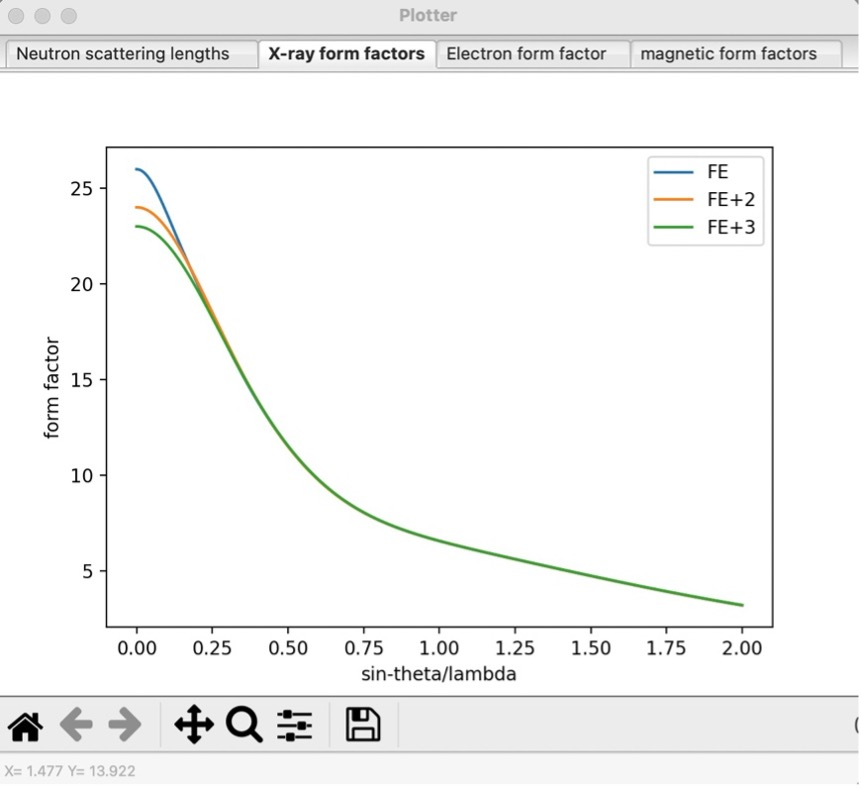
\includegraphics[width=0.6\linewidth]{figures/Diffract1.jpg}
    \caption{Plot of x-ray form factors for Fe, Fe\textsuperscript{2+} and Fe\textsuperscript{3+} from GSAS-II program PlotXNFF}
    \label{fig:diff1}
\end{figure}
Despite my comments, if one persists in using charged-atom scattering factors, a common question will be ``what should I use for a species that is not provided, such as Fe\textsuperscript{+4}?'' Certainly, form factors for Fe\textsuperscript{+3} and Fe\textsuperscript{+4} will be just about the same except at very low Q. Feel free to substitute a similar valence scattering factor curve. Achieving charge balance for scattering factor selection is not important, since again this only affects low-angle scattering and again only in a second-order fashion. 

\subsection{Neutron Scattering Cross Sections}

 In contrast to x-rays, neutrons are usually scattered from the nucleus of the atom, and this scattering can usually be considered as a point-point interaction that does not vary with the angle of scattering. The probability for this type of scattering is thus a constant independent of angle, but does depend on the neutron energy and, in particular, on the interactions at the quantum level between the nucleus of the atom and the neutron, which depends on the isotope of the atom. In fact, the scattering probability may be very different for isotopes of the same element. The scattering probability for neutrons is commonly referenced as a cross-section, $\sigma$,\index{scattering cross-section} with units of area (length\textsuperscript{2}). There is also a quantity related to the square-root of the cross-section, which is called the scattering length, \textit{b},\index{scattering length} and has units of length. Finally, while all atoms scatter x-rays with no phase inversion, most isotopes do scatter neutrons with phase inversion, but a few do not. For those unusual isotope types that do not invert the scattering phase, we indicate this using a negative value for \textit{b}. 

There are separate probabilities for coherent and incoherent neutron scattering, which can vary greatly. As a fairly extreme example, the coherent and incoherent scattering lengths for the \textsuperscript{1}H isotope of hydrogen are -3.7406 fm and 25.274 fm, respectively. Since scattering probabilities go as the square of the scattering lengths, a neutron is $\approx$45 times more likely to be scattered incoherently than coherently by a \textsuperscript{1}H atom. As was discussed previously, this incoherent scattering occurs at all diffraction angles and adds greatly to the background, making it much harder to measure diffraction with significant precision in the presence of a significant atomic percentage of \textsuperscript{1}H. For this reason, samples containing deuterium (\textsuperscript{2}H), for which the coherent and incoherent scattering lengths are 6.671 fm and 4.04 fm, respectively, are greatly preferred for neutron diffraction. 

Noting that almost all elements exist as a mixture of isotopes, the net coherent scattering from any element is dependent on the weighted sums of the scattering lengths, which can work towards canceling each other if the signs of \textit{b} are opposite. While normally \textsuperscript{2}H is only 0.015\% of the natural isotopic makeup of hydrogen, if we enrich the level of \textsuperscript{2}H to 36\% at a site, we have a net coherent scattering of 0.0075 fm [ = (‑3.7406*0.64) + (6.671*0.36)], meaning that there is nearly no coherent scattering from this site. The overall probabilities for scattering from the \textsuperscript{1}H and \textsuperscript{2}H atoms are unchanged by their mixture, but all of their scattering now becomes incoherent. A similar effect occurs with vanadium, which at natural isotopic composition is 0.25\% \textsuperscript{51}V with \textit{b}= 7.6 fm and the remainder \textsuperscript{50}V with \textit{b} = -0.402 fm. Note that (0.25*7.6 + 99.75*-0.402)/100 = ‑0.382 fm, which is a relatively weak diffracting material. Vanadium is a preferred as a container material for neutron diffraction, due to the very small levels of diffraction seen from that metal. 

Note that there are potentially two ways that incoherent scattering can arise. It can be an intrinsic property of the neutron-nucleus interaction, typified by \textsuperscript{1}H, but can also arise from having a mixture of isotopes. GSAS-II provides coherent neutron scattering lengths for elements at natural abundance and for isotopes where the scattering lengths have been reported in the literature, so it is not necessary to look up any of these values.

There is one common exception to the angular-independent scattering of neutrons by atoms, and that occurs in materials with ordered unpaired electrons. Depending on the type of ordering, materials with unpaired electrons may be ferromagnetic, paramagnetic or exhibit related types of magnetic phenomena such as ferrimagnetism. Unpaired electrons have a net spin, as do neutrons, and these unpaired electrons can scatter neutrons from this spin-spin interaction. These unpaired electrons are always valence electrons and thus are more dispersed from the nucleus than the average for all the electrons. This means that scattering of neutrons by unpaired electrons falls with increasing angle similarly to what is seen in x-ray scattering, but the decrease with Q is even faster for magnetic neutron scattering than what is seen in the form factor for x-rays. Different scattering length curves are tabulated for different valence states for atoms that exhibit magnetic effects. These are automatically assigned in GSAS-II when a material with magnetic scattering is defined. 
In GSAS-II to change the valence state for an atom, click on the type entry in the Atoms table. This brings up a periodic table and under each element there are choices for valence state.

\section{Resonant scattering}

As mentioned previously, scattering from an atom involves components in the real and complex planes. This becomes of particular importance when considering scattering at resonant edges, meaning where the energy of an x-ray photon is close to that for an absorption edge for a particular element. When x-rays are scattered near an atom’s absorption edge, the scattering can be described by adding two additional components for scattering in the real and imaginary planes, so the total form factor f\textsubscript{tot}($\lambda$,Q) is written as \textit{f}\textsubscript{tot}($\lambda$,Q) = \textit{f}(Q) + \textit{f}’($\lambda$) + \textit{i}\textit{f}’’($\lambda$). This effect of wavelength on scattering is usually called anomalous dispersion in chemical crystallography and resonant scattering in physics.\index{anomalous dispersion|textbf}\index{resonant scattering|textbf}\label{ref:resonantscattering} I think that resonant scattering seems a much better term to use. The values of \textit{f}’ and \textit{f}’’ are normally quite small, but can reach an electron or two close to absorption edges, which means they are still not large, but do become experimentally significant. 

In a resonant scattering experiment, one collects two datasets, one at a wavelength close to (but still somewhat below) an absorption edge for an element and another at a similar wavelength, but well away from an absorption edge. Since the only significant change between the two patterns will be the scattering from the element at this selected edge. This “tweaking” of the scattering for a particular element can be thought of as akin to the derivative of the diffraction pattern with respect to the element in question, but in GSAS-II one analyzes the data by fitting both datasets against a single model. Note that the values for f’ and f’’ and in particular the exact location of the absorption edge will be dependent on the chemical environment for the selected element, but 100 eV below the edge, the values are pretty much independent of the bonding details. 
Prior to synchrotrons, resonant scattering diffraction experiments were nearly impossible, now they are possible, but are still uncommon as few if any synchrotron diffraction beamlines are designed to change x-ray wavelengths easily. 

 In GSAS-II the values for \textit{f}’ and \textit{f}’’ are computed using the tabulation of D.T. Cromer and D. A. Liberman and are automatically computed for every appropriate element based on the supplied x-ray wavelength. The GSAS-II program Fprime\index{software!Fprime} (in the Calculate menu) shows the values computed with this tabulation as a function of x-ray wavelength. As noted, these values are only approximate near the edge, but where resonant scattering measurements are normally made, circa 100 eV below the resonant scattering edge, the values are largely not highly dependent on the species’ chemical environment and should be reasonable approximations. If greater accuracy is needed, when a resonant scattering experiment is done, one should consider collecting a wavelength-dependent fluorescence or absorption measurement. From this using a Kramers-Kronig inversion one can compute the \textit{f}’ and \textit{f}’’ curves for the specific material being studied as a function of wavelength. This would need to be done outside of GSAS-II. 

 A similar resonant scattering effect can also occur when neutron energies that match absorption edges for particular isotopes, but this is far less common and typically occurs at relatively high neutron energies that are seldom accessible in diffraction experiments, but there are a small number of elements that offer exceptions. GSAS-II uses tables computed by Lynn and Seeger to compute nuclear resonant scattering. The values generated from those tables can be also viewed in program PlotXNFF, as shown in Fig. \ref{fig:diff2}. Nuclear resonant scattering is usually an issue only with the higher energy neutrons available at spallation sources, but that can pose a problem since some TOF instruments sum together data acquired over a wide of range of detector angles. This mixes together diffraction from different wavelengths making treatment of resonance in the form factor impossible. 

 \begin{figure}
    \centering
    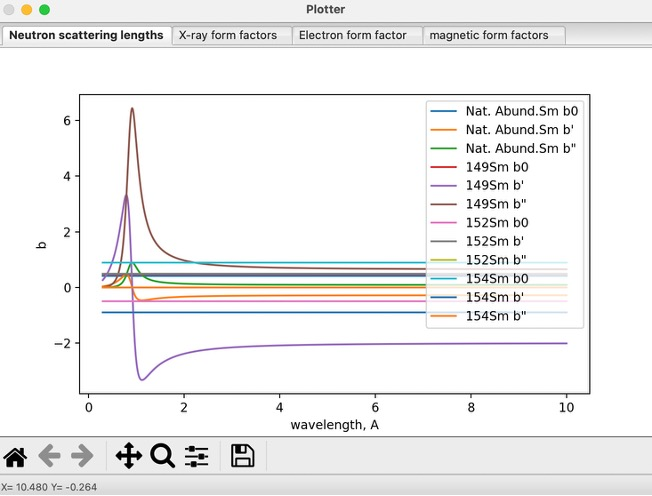
\includegraphics[width=0.6\linewidth]{figures/Diffract2.jpg}
    \caption{Resonant neutron scattering for isotopes of Sm as a function of wavelength as plotted by program PlotXNFF}
    \label{fig:diff2}
\end{figure}

\section{Diffraction from materials}

 Diffraction occurs when a pair of atoms are spaced apart so that their scattering is in phase and thus can add at an appropriate angle. At other angles, the scattering will not have this constructive interference and will on average cancel. A completely random arrangement of atoms would have pairs of atoms at all distances and thus would be expected to have completely uniform diffraction (following the form of \textit{f} with angle) at all scattering angles. However, matter never has a completely random arrangement of atoms. Even gases have some ordering, since atoms can never approach too closely and thus even diffraction from gases will show some level of structure. 
 
Peter Debye\index{Debye, P.} in 1915 first tabulated an equation that computed diffraction intensity as a function of the distances between pairs of atoms in a sample. His equation can be rewritten in a slightly different but more convenient form as: \index{Debye equation|textbf}
$$I\left(Q\right)=Nf^2\sum_{i}^{N}\sum_{j\neq i}^{N}\frac{\sin{Qr_{ij}}}{Qr_{ij}}$$
where r\textsubscript{ij} is the distance between atoms i and j. In this equation, \textit{f} indicates the scattering power for each atom, discussed previously as the form factor or scattering length, and \textit{I(Q)} will be the relative intensity for scattering per unit solid angle. N is the total number of atoms and thus this is a double sum that would include \textit{every} pair of atoms in the sample, which is intractable for any reasonable number of atoms. In practice, since the sinc function [$\operatorname{sinc}(q,r) = \sin(qr)/qr$] falls to very small values as qr becomes large, it is not necessary to consider pairs of atoms at very large distances. This equation (or equations derived from the Debye equation) allow for computation of diffraction scattering from disordered materials, such as glasses, but can be simplified greatly for crystalline materials as will be discussed further below. 

\section{Absorption and Extinction}

As we saw before, neutron or x-ray quanta can interact with the sample in several ways. Alternatively, they may also not be scattered at all and go straight through the sample unperturbed. When quanta are scattered incoherently or inelastically or are captured by the sample, they can no longer contribute to the diffraction signal. Diffraction intensities are computed ignoring this effect, but when samples have high probabilities for neutron or x-ray absorption or non-diffraction scattering, the fraction of lost quanta will depend on the scattering geometry, the wavelength and the diffraction angle. If a significant fraction of the quanta are absorbed or are otherwise scattered by non-diffraction events, a correction factor may be needed to accurately match the idealized diffraction intensities to what is actually observed. This is known as an absorption correction, but it should be noted that non-diffraction scattering as well as actual absorption is corrected for in this factor. To evaluate the effects of absorption, GSAS-II includes a program (also in the Calculate menu) called Absorb\index{software!Absorb} where a chemical formula is supplied along with a sample size and density or packing fraction (since powder samples usually are not fully dense) and the value of $\mu r$ is computed as function of wavelength. Absorption corrections are discussed in more depth in \S\ref{ref:Absorption}.

Another assumption that is made when computing diffraction intensities is that the probe quanta are only scattered once and only a small fraction are scattered. In an effect called multiple scattering, it is possible for a scattered quantum to be scattered again before it leaves the sample. This occurs most significantly for intense reflections in large single crystals and this effect is called primary extinction. This effect is greatest when crystals have very large domains, without defects to disrupt ordering. To compute primary extinction quantitatively, one must use a higher level of scattering theory than will be discussed here, called dynamical diffraction. Note that primary extinction can be quite significant in electron diffraction because with the high electron energies used, only small domains within a sample are probed and are much more likely to have “perfect” ordering on these distance scales. 
 
Another effect can occur, similar to absorption, if significant fraction of the incident quanta are diffracted before many of the particles penetrate into the sample. The result of this is that fewer quanta are available to be scattered than will be expected. This is known as secondary extinction. 

Both primary and secondary extinction are most likely to be observed with large and highly perfect crystals. More commonly, so-called single crystals are actually constructed of relatively small domains due to defects and these domains have small misalignments with each other. Such a crystal is known as ideally mosaic. The small domain sizes disrupt the dynamical scattering needed to cause primary extinction and the small misalignments between domains prevent secondary extinction. Single-crystal experiments will sometimes benefit if a crystal is thermally shocked to induce mosaicity. However, extinction is quite rare in powder diffraction because when crystallite sizes are larger than a few microns, sample grinding should be used. GSAS-II does provide correction terms for extinction that can be used for both single-crystal and powder diffraction and with both x-rays and neutron. While rarely needed, these do work well for materials with very large crystallite sizes. Note that laboratory powder diffraction experiments with such large-grain materials are likely to be inaccurate, due to poor particle counting statistics, but this is less likely to be a problem with high-energy x-rays and neutrons.  

\section{For More Information}

\begin{itemize}
\item \textit{Fundamentals of Crystallography.} Third Edition (2011). C. Giacovazzo, H. L. Monaco, G. Artioli, D. Viterbo, M. Milaneso, G. Ferraris, G. Gilli, P. Gilli, G. Zanotti and M. Catti. Edited by C. Giacovazzo. IUCr Texts on Crystallography No. 15, IUCr/Oxford University Press.
\begin{quote}
This is a weighty, comprehensive, and modern book on crystallography. If you are going to buy anything, this is what I would recommend. 
\end{quote}

\item\textit{Elements of X-Ray Diffraction}, 3rd Edition (2014), B.D. Cullity and S.R. Stock. Pearson. 
\begin{quote}
This is a general x-ray diffraction text that is more oriented to materials studies than most. Commonly used as a teaching textbook. Despite the publication date, it was last revised in 2001, I believe.
\end{quote}

\item \textit{International Tables for Crystallography
Volume C: Mathematical, Physical and Chemical Tables}, (2021) T. R. Welberry ed.\\ 
DOI: 10.1107/97809553602060000117
\begin{quote}
This is a comprehensive and pricey reference on all types of diffraction, with tables and articles on practically everything, but is probably much more than you want. Your library/institution may have arranged on-line access, even if they don't have a print copy. 
\end{quote}
\end{itemize}

\chapter{Crystallographic Symmetry}

\section{The lattice}

Moving from interactions of quanta and matter, let us consider how atoms are arranged in matter. Atoms exist in a quantum-level universe as well, and repel each other if they are placed too close, but attract each other at longer distances. They can also create lower-energy structures by sharing electrons (chemical bonding) to form molecules or for unbonded charged objects, packing in three dimensions in a way to best alternating charge can also reduce the energy (a simple way to consider this is via the Madelung potential). 
In general, enthalpy is lowered when atoms and molecules self-arrange in dense and regular three-dimensional patterns. Opposing this is entropy, which is increased by randomness. 
In the macroscopic world that we live in, entropy and enthalpy balance at equilibrium, and all materials, even away from equilibrium, exist with both order and disorder present. 
Nonetheless, it is worthwhile considering the properties and symmetry of a perfectly organized set of atoms or molecules, which we will call an ideal crystal, even though it is an imaginary concept; no perfectly ordered materials exist. 

In an ideal crystal, atoms occur only at a set of fixed distances from each other, and the structure is built up of repeating units. 
For the purposes of this introduction, I will not consider two important forms of crystalline matter, quasicrystals and modulated structures, as these require descriptions in more than three dimensions. 
Quasicrystals are composed of atoms that organize in long-range patterns, but these patterns do not repeat in regular units. 
In 1982 Dan Shechtman\index{Schectman, D.} found clear evidence for such a material, and despite rejection from a significant and highly vocal segment of the scientific community (typified by a comment attributed to Linus Pauling\index{Pauling, L.} that “there are no quasicrystals, only quasi-scientists”) continued to speak to what he had observed in an electron microscope. 
The existence of quasicrystals\index{quasicrystal} is now fully accepted, and Shechtman was awarded a solo Nobel prize in 2011. 
Similarly, in modulated structures, incommensurate ordering is superimposed on regular three-dimensional patterns of repetition. 
While initially, the definition of what we would call crystalline matter was tied to the existence of long-range repetition units of atoms, now the definition has been expanded to any matter that shows long-range atomic organization through the appearance of a sharp diffraction pattern. 
Since my goal here is to explore the properties from long-range repetition units of atoms and show how sharp diffraction patterns arise from this, I will only consider classical three-dimensional ideal crystals and will use them to introduce two initial concepts, the lattice and the reciprocal lattice. 

Our imaginary idealized crystal is built of repeated three-dimensional identical boxes of atoms. 
At this stage, we do not need to concern ourselves with how the atoms are arranged within each box, but we will stipulate that identical means this arrangement is repeated exactly in every box. 
The crystal is built up by these boxes stacked in every direction. 
It has been known since the 1800’s that there are seven shapes of boxes that can be used to build a larger object without any gaps. 
In the simplest example this box would be a cube – having equal length sides and all angles between sides as multiples of 90 degrees. 
However, these requirements on dimensions and angles can be relaxed, giving rise to a total of seven options, as listed in the Table \ref{tab:constraints};\footnote{Note that conventionally the term rhombohedral is used for both a class of lattice symmetry, that can occur with two different types of unit cells, or a unit cell that has three equal cell lengths and cell angles; to differentiate the latter, I reserve rhombohedral for symmetry and rhombohedric for the unit cell type.} this gives rise to what is known as the \textbf{seven crystal systems}\index{crystal systems}. 
These boxes are all parallelepipeds, meaning six-sided objects where there are three pairs of parallel sides. 
Note that while one can tile space with hexagons (or in three dimensions, hexagonal prisms), we consider the hexagonal crystal systems to be constructed from parallelepipeds with two equal sides that have a 120° angle between them and where the third side is perpendicular to the other two. 
Three of these parallelepipeds can construct hexagonal prisms. 
Thus, this parallelepiped description is equivalent to one built from hexagonal prisms. 

\begin{table}
\centering
\caption{The seven crystal systems and their constraints.}
\label{tab:constraints}
\begin{tabular}{| l | p{0.25\textwidth} | p{0.4\textwidth} |}
\hline
Name & Constraints on lengths of sides & Constraints on angles between sides \\
\hline
Cubic & All three equal & All 90 degrees \\
\hline
Tetragonal & Two must be equal & All 90 degrees \\
\hline
Orthorhombic & none & All 90 degrees \\
\hline
Hexagonal & Two must be equal & 120 deg. between equal sides; 90 deg. for other two \\
\hline
Rhombohedric & All three equal & Any, but all three must be equal \\
\hline
Monoclinic & none & Any for one, 90 deg. for other two \\
\hline
Triclinic & None & None \\
\hline

\end{tabular}

\end{table}

 Armed with the concept of crystal systems, we can define an important term in crystallography, that of a \textbf{lattice}\index{lattice}. 
Let us label one arbitrary point in the box. 
The point we select might be a corner but could also be some location inside the box. 
For that selected point, we can envision that there will be a fixed arrangement of atoms around that point. 
Should we move to the same point in any other box, the arrangement of atoms will be identical since the boxes are all identical. 
If we then imagine selecting that same point in every box, we construct an infinite network of indistinguishable points. This infinite network of points is called the lattice. For a given arrangement of atoms, there are any number of ways to construct the lattice, since we can choose any point in the box as our reference point. We could also choose a more sparse network of points, such as selecting every other point in some direction and thus enlarge our box, but still we can decorate our infinite crystal from that lattice. Thus, there are an infinite number of possible lattices associated with a structure. We will see later that only some will better describe the symmetry of the structure. The term lattice is commonly misused to describe the structure or chemical makeup of the crystal, with poorly considered terms such as “lattice compound.” In truth, a lattice is just a mathematical concept, simply a collection of points. 

\section{The unit cell and fractional coordinates}

 For the box we used to construct our ideal crystal, we give the name the \textbf{unit cell.}\index{unit cell}
 We still need not consider exactly how the atoms are arranged within that box, but since every box (or equivalently unit cell) is identical, once we have described the contents of the unit cell, we can construct an exact description of the entire crystal. 
 This leads to a very convenient mechanism for describing the coordinates of atoms within the unit cell using \textbf{crystallographic axes}, which are also sometimes called the \textbf{crystal axes}. We label the three sides of the unit cell as \textbf{\textit{a}, \textit{b} \& \textit{c}}\index{\textit{a}}\index{\textit{b}}\index{\textit{c}}, and define the angles between the sides as \textbf{α}, \textbf{β}, \& \textbf{γ}\index{$\alpha$}\index{$\beta$}\index{$\gamma$}, where we define as γ the angle between the \textit{a} \& \textit{b} sides, β between \textit{a }\& \textit{c}, and α between \textit{b} \& \textit{c}. We then define \textbf{axes}, \textbf{x, y \& z} along \textit{a}, \textit{b} \& \textit{c} directions, respectively. Note that the angles between these axes are dictated by α, β \& γ, so for systems other than cubic, tetragonal and orthorhombic, angles between axes may not be 90 degrees. Such axes systems are \textit{non-orthogonal} (also called oblique) which makes performing three-dimensional algebra more difficult, but will so greatly simplify our descriptions of the crystal that this mechanism is much preferred over orthogonal coordinate systems. Table \ref{tab:conventions} outlines the common conventions used for assigning axes for the seven crystal systems.
 
\begin{table}
\centering
\caption{Conventions for labeling of axes for the seven crystal systems.\index{crystal systems} Note that for monoclinic systems, the convention below is the current conventional preference, but \textit{c} unique (where α = β = 90°) was more commonly used historically. Use of \textit{a} unique (β = γ = 90°) is seen in the literature only rarely.}
\label{tab:conventions}

\begin{tabular}{| l | p{0.2\textwidth} | p{0.3\textwidth} |}

\hline
Crystal system name & Constraints on lengths of sides & Constraints on angles between sides \\
\hline
Cubic & \textit{a}=\textit{b}=\textit{c} & α = β = γ = 90° \\
\hline
Tetragonal & \textit{a}=\textit{b} & α = β = γ = 90° \\
\hline
Orthorhombic & none & α = β = γ = 90° \\
\hline
Hexagonal & \textit{a}=\textit{b} & γ = 120°; α = β = 90° \\
\hline
Rhombohedric & \textit{a}=\textit{b}=\textit{c} & α = β = γ \\
\hline
Monoclinic & none & b unique: α = γ = 90° \\
\hline
Triclinic & none & none \\
\hline

\end{tabular}

\end{table}

 Finally, we scale each axis so that one unit of length corresponds to the length of the unit cell in that direction. This means that for most crystal systems the per unit along each axis may differ, so This means that we can label any point inside the unit cell with coordinates (x,y,z) where $0\leq \rm x<1$, $0\leq \rm y<1$ and $0\leq\rm z<1$. Locations on the faces of the unit cell will have $\rm x=0$ or $\rm y=0$ or $\rm z=0$ and the coordinates for the eight corners of the unit cell are (0,0,0), (1,0,0), (0,1,0), (0,1,0), (1,1,0), (1,0,1), (0,1,1) and (1,1,1). The center of the unit cell is (0.5, 0.5, 0.5). This system of coordinates is known as \textbf{fractional coordinates}.\index{fractional coordinates} We can also consider the location of a point inside the cell with location (x,y,z) as a vector from the origin to the atom position, $\vec{x_{xyz}}=\ x\hat{a}+\ y\hat{b}+z\hat{c}$ where $\hat{a}$, $\hat{b}$ and $\hat{c}$ are unit vectors (\textit{i.e.} with length in the same units, for example, Å) in the appropriate direction.

 Note that since the contents of every unit cell is the same, adding or subtracting any multiple of 1 to x, y and/or z results in a location that is indistinguishable from the initial point. We can write a rule that point (x,y,z) is equivalent to (x+n\textsubscript{x}, y+n\textsubscript{y}, z+n\textsubscript{z}) where n\textsubscript{x}, n\textsubscript{y} and n\textsubscript{z} can each be any integer to express the superposition of the infinite lattice replicating the contents of the unit cell in all directions. 

\section{Fourier Space}

 Before covering an important concept in crystallography, the reciprocal lattice, it is worthwhile to consider a Fourier transform\index{Fourier transform} and its implications for coordinate systems. This is one of many ways to write a Fourier series\index{Fourier series}:

$${I(x)}=\sum_{N=-\infty}^{\infty}f_N\exp⁡[2\pi\ iNx/P]$$

In this $I(x)$ is a function that is periodic in P, meaning that $I(x) = I(x+P)$. The physical importance of this is that any periodic function can be constructed by adding together exponential (or equivalently sine and cosine) functions, where the lowest order function has the same periodicity as the original periodic function (where \textit{N} is 1) and all the remainders are harmonics of that, where the periodicity is double, triple,… (thanks to the \textit{N} term.) 

The best example I can offer for the use of the Fourier transform in one dimension has to do with sound. As we know, musical instruments can all play the same notes, where a note has a defined frequency, or equivalently wavelength, but can sound very different: consider the “pure” sound of a middle-C note on from a flute in comparison to the very “brassy” sound of a middle-C from a saxophone. We can build either sound from adding together sine waves with the frequency of middle-C (usually 262 Hz) and its harmonics (524 Hz, 786 Hz,…). The harmonics are each an octave above the original note, so we can create the sound of our saxophone by adding together “C’ notes with varying amplitudes, as well as some other overtones with related frequencies. (The flute is already very close to a pure sine wave). Thus, we have taken a complex time-varying wave form and expressed as a mixture of components described by frequency. 

The Fourier transform takes a signal in units of time, and expresses it as a function in frequency (1/time). This is the magic property of a Fourier transform that it allows us to go between two sets of coordinates, where one is the inverse of the other. This relationship is described by saying that frequency is the Fourier conjugate of time. This relationship exists not only for one dimensional functions, but also can be expressed in higher dimensions, for example for a three-dimensional (or even six-dimensional) periodic function. We call the domain of the Fourier component functions, which have inverse units from our original function, as operating in “Fourier space”.

\section{The reciprocal lattice}

Since crystallographic axes may be non-orthogonal, we can make some calculation processes much simpler by describing a new set of axes relative to the previously defined crystal axes, which we call the \textbf{reciprocal lattice}\index{reciprocal lattice}. 
To define the reciprocal lattice, we create three new axes, which we label as \textbf{\textit{a*}, \textit{b*} }\&\textbf{ \textit{c*,}}\index{\textit{a*}}\index{\textit{b*}}\index{\textit{c*}} where the asterisk (*) indicates these are reciprocal lattice axes. We make these axes perpendicular to the plane containing each pair of the crystal system axes (\textit{a}, \textit{b} \& \textit{c}), meaning that \textbf{\textit{a* }}is perpendicular to \textit{b} \& \textit{c}, and likewise for\textit{ \textbf{b* }}to \textit{a} \& \textit{c }and \textbf{\textit{c* }}to \textit{a} \& \textit{b,} or equivalently using dot products to designate perpendicular axes, $a^*\cdot b =  a^* \cdot c = b^* \cdot a =  b^* \cdot c =  c^* \cdot b =  c^* \cdot a = 0$. We also scale the length of the reciprocal axes so that $a^*\cdot a = 1$, $b^*\cdot b = 1$ and $c^*\cdot c = 1$. Note that since we conventionally use units of Ångstroms (Å) for \textit{a}, \textit{b} \& \textit{c}c, then the units of \textit{a*}, \textit{b*} \& \textit{c*} are Å\textsuperscript{-1}. The angles between the reciprocal aces, \textbf{α*, }\textbf{β* \& }\textbf{γ*}\index{$\alpha^\ast$}\index{$\beta^\ast$}\index{$\gamma^\ast$} are defined analogously to the angles for the crystal axes so that \textbf{α*} is the angle between \textit{b} and \textit{c}, etc. 

 The properties of this new reciprocal axis coordinate system were first discovered by J. Willard Gibbs\index{Gibbs, J. W.}, well in advance of modern crystallographic practice. This coordinate system turns out to be the ideal mechanism to describe the three-dimensional conjugate space needed for Fourier analysis of the periodic density of scatterers in the unit cell. The reciprocal axes are also used to formalize a concept called the Ewald sphere, which is used to understand the orientation needed to bring a single crystal into a diffracting position, as well as which diffraction maxima can be observed with a given wavelength particle. While elegant, the Ewald sphere is not really needed for powder diffraction. For our purposes, we will only consider that diffraction occurs in only with reciprocal lattice with $\vec{d_{hkl}^\ast}=\ ha^\ast+\ kb^\ast+lc^\ast$, where \textit{h, k}, and \textit{l} are all integers. 

 We will call this domain of this reciprocal lattice construct as \textbf{reciprocal space} and correspondingly, the domain where atoms are located is called \textbf{real space}. Note that perhaps confusingly, I have followed conventional use and now used the term “real” in three different contexts. One as “real numbers”, as in the opposite of imaginary numbers for complex algebra (involving $i=\sqrt{-1}$), another as “real space” to be distinguished from the reciprocal space construct we just introduced. Finally, I use “real” sometimes to make clear the properties of actual materials in comparison to our idealized concepts.

 Just as we measure bond distances between atoms in real space, there are some commonly referenced quantities in reciprocal space. 
 As noted before, if we define a reflection direction as vector $\vec{d_{hkl}^\ast}=\ ha^\ast+\ kb^\ast+lc^\ast$, we can also consider the magnitude of that vector, $d_{hkl}^\ast=\left|\vec{d_{hkl}^\ast}\right|$, which will have units of inverse length (typically Å\textsuperscript{-1}). 
 This is often written without the subscripts as \textit{d*}.\index{d*} 
 As will be seen, this quantity is used in Fourier transform relationships where a factor of 2π is commonly required. 
 Physicists typically prefer the quantity $\rm Q$\index{$\rm Q$}, where Q = 2π d*. In addition to Q and d*, there is one more widely-used quantity that I personally would prefer to see disappear from usage. This is the quantity \textbf{d} and is often called a \textbf{d-space}, where d = 1/d* = 2π/Q. The units of d thus are length, but note that d is actually measuring a quantity that is only meaningful in reciprocal space. I do not like use of d (d-space values) because it tempts one to use that real space length to relate some aspect of the atomic structure to the scattering at a location in reciprocal space, but this ignores that scattering intensities and the atomic structure are in a Fourier relationship, where every aspect of the structure affects the scattering to some extent. The wide use of d is somewhat historical, since it is part of \textbf{Bragg’s law}, ($n\lambda=2d\sin{\theta}$)\index{Bragg's law}. This equation had already been used to describe the properties of waves. In this equation λ is the wavelength for the scattered particle, θ is one-half the angle between the incident direction of the particle and its scattered direction. The factor \textit{n} here is due to the idea the diffraction occurs at orders with integer multiples, but since we build that into the \textit{hkl}values, we can treat \textit{n} as unity and remove it. As much as I respect the amazing sagacity of William Laurence Bragg\index{Bragg, W. L.}, I would prefer that this formulation of Bragg’s law be replaced with $\lambda={2\sin\theta}/{d^\ast}$ or $\lambda ={2\pi\sin\theta}/Q$. To understand why Bragg’s law was such an important advance, it should be understood that this wave equation went against the thinking of many established scientists, including his father William Henry Bragg, who did not believe that x-rays had wave character. Laurie Bragg\index{Bragg, W. H.} deployed that wave equation at age 22 and won a well-deserved Nobel prize at a ripe old age of 25. Bragg’s law was intended to relate scattering of x-rays to distances between planes of atoms, which we now can see is a poor idea as it confuses direct and reciprocal space phenomena. 

 As has been mentioned, while diffraction patterns are commonly measured in units of 2θ, this means that the measurement results change depending on the wavelength of the source. 
 As noted, in energy-dispersive detection measurements are made at constant 2θ with measurement of $\lambda$. So that diffraction data may be compared with different data collection types and different wavelengths, display of patterns in units of Q rather than 2θ is a wise choice. Q also has the advantage that it roughly scales with 2θ, so that if one refers to low Q, that can be readily interpreted as low angle scattering, while high Q will refer to high angle scattering (or perhaps unobservable, except with shorter wavelengths.)

\subsection{The cell and reciprocal-cell tensors}

To simplify the algebra used with lattice computations, GSAS-II uses a series of tensors that allow for simple and quickly-computed linear algebra expressions to perform what would otherwise be fairly complex expressions. 

The [direct] cell tensor, $g$, is defined as, 
$$
   g = \left( \begin{matrix}
   a^2 & a b\cos\gamma & a c\cos\beta \\
   a b\cos\gamma & b^2 & b c \cos\alpha \\
   a c\cos\beta &  b c \cos\alpha & c^2
   \end{matrix}\right)
$$
Note that for higher-symmetry unit cells, $\alpha$, $\beta$ and/or $\gamma$ may be $90^\circ$ and $\cos90^\circ$ is zero, so that some or all off-diagonal terms become zero. 
The reciprocal cell tensor, $G$\index{$G$}\index{reciprocal lattice tensor}, is defined as the inverse of $g$, $G = g^{-1}$. This allows us to simplify the expression for $|\vec{d_{hkl}^\ast}|$ (where $\vec{d_{hkl}^\ast}=\ ha^\ast+\ kb^\ast+lc^\ast$) as 

$$|\vec{d_{hkl}^\ast}| =  Q / (2 \pi) =  \sqrt {G_{11} h^2 + G_{22} k^2 + G_{33} l^2 + 2 G_{12} hk + 2 G_{13} hl + 2 G_{23} kl}$$

Another quantity based on $G$ is used throughout GSAS-II for lattice fitting. We call this the $A$ matrix\index{$A$ matrix} and is defined as
$$ A = \begin{matrix} G_{11} & G_{22} & G_{33} & 2G_{12} & 2G_{13} & 2G_{23}\end{matrix}$$ 
Numbering the terms in $A$ to start with zero, as is done in Python, the length in reciprocal space simplifies to

$$Q = 2 \pi \sqrt {A_0 h^2 + A_1 k^2 + A_2 l^2 + A_3 hk + A_4 hl + A_5 kl}$$ 

\section{The structure factor equation}

Armed with this all this nomenclature we can formulate a much simpler expression than the Debye equation\index{Debye equation} for the scattering from a crystal, since we only need to consider the atoms in one unit cell. As was mentioned, the scattering from a perfect crystal can be described as diffraction that occurs at discrete spots and those spots can be indexed by three numbers, (\textit{h, k, l}), that represent a direction in reciprocal space, $ha^\ast+\ kb^\ast+lc^\ast$. I will use the historical (and misleading) term of “reflections” for those spots. The choice of the term reflection was a questionable choice since the physics of diffraction has nothing to do with the physics of reflections of light, such as when we see ourselves in a mirror. Nonetheless, it is a widely accepted terminology that I will not fight against. 

A useful quantity for understanding reflections is called the \textbf{structure factor}\index{structure factor}\index{$F_{hkl}$}, \textit{F}\textsubscript{hkl}, which represents the scattering amplitude and phase for each reflection. 
This takes into account the scattering from every atom in the unit cell, where  
$$F_{hkl}=\ \sum_{ij}^{N}{f_i\exp(-2\pi i\vec{d_{hkl}^\ast} \cdot  \vec{x_{j}})}$$

where $\vec{d^*_{hkl}}$ is the vector in \textit{reciprocal space} for reflection (\textit{h, k, l}) and $\vec{x_j}$ is the vector from origin to the atom location \textit{in real space}. Now we can see the value of the reciprocal space construct from how it simplifies the dot product. The quantity $\vec{d_{hkl}^\ast}\cdot\vec{x_j} = hx_j+\ ky_j+lz_j$, even for a triclinic system because between the reciprocal lattice was defined so that \textit{a*}\textit{·b} = \textit{a*}\textit{·c} = … = 0 and \textit{a*·a}= … = 1. Note that F\textsubscript{hkl} values will be complex numbers where the relative values of the real and imaginary components and their signs indicate a phase. The magnitude of the structure factor, |\textit{F}\textsubscript{hkl}|, describes the strength of this particular diffraction peak. Conversion of |\textit{F}\textsubscript{hkl}| to the actual intensity observed for the Since \textit{hkl} indicates a direction in reciprocal space, we can think of F\textsubscript{hkl} as describing both the strength and phase for scattering in the \textit{hkl} direction. Note that our previous definitions for reciprocal space require \textit{a*·b} = \textit{a*·c} = 0 and \textit{a*·a} = 1 (and likewise permuted with \textit{b}* and \textit{c}*) and this means that ($\vec{q_{hkl}}\cdot\vec{x_i}$)  can be simplified to (\textit{h}x\textsubscript{i} + \textit{k}y\textsubscript{i} + \textit{l}z\textsubscript{i}). Thus, the structure factor can be rewritten as 

$$F_{hkl}=\sum_j^N f_j \exp⁡[-2πi(hx_j + ky_j + lz_j)]$$

Note that while the Debye equation\index{Debye equation} is a double sum over \textit{all atoms in the material}, this equation is a single summation over only the atoms \textit{in the unit cell}.
In very approximate terms, this has reduced the complexity of the computation by a factor of 10\textsuperscript{40} for the dimensions of a real sample. 
Note also that the observable intensities of reflections will depend on the square of the structure factor, as well as experimental effects depending on how the measurement is performed. 

\section{Site Occupancies}\label{ref:occupancies}
One factor that must also be considered is that sometimes there can be random distributions of either vacancies, where an atom is missing from a site, or site substitution, where one element substitutes for another. In some cases, both occur together. If these distributions were ordered, this would mean that the symmetry would be lowered, but if the vacancies and/or substitutions are random, the symmetry is not affected. The effect of vacancies is to reduce the $f_j$ value linearly, e.g.  $f_j$ is replaced by  $o_j f_j$ where $o_j$ is a number between 0 and 1. If two or more atoms share a site, one adds extra terms to the summation and the sum of the  $o_j$ values for the atoms that share a site must be between 0 and 1. As will be discussed later, one frequently makes the assumption that the sum is 1 because it requires multiple measurements to demonstrate any other value. 
 

\section{Ideal vs. real crystals}
Of course, our imaginary ideal crystal differs from real-world crystals in many ways. One way that real crystals differ from our idealized concept is that atoms are constantly in motion. Usually, this motion is such that the atoms vibrate around some point in the structure so that the time-averaged positions are the same from one unit cell to the next. Since the overall amount of vibration is determined by the temperature of the material, this is called thermal motion\index{thermal motion} but this motion does not completely disappear at lower temperatures and if 0 K were achievable, atoms would still have what is called zero-point motion. These instantaneous deviations from ideal siting are called dynamic disorder. The intensities of reflections are lowered because this thermal motion spreads out the siting of the nucleus or electrons over some region and this preferentially lowers the intensities of the higher Q reflections for the same reason as why \textit{f}(Q) decreases with angle in x-rays. This was noted and explained very early in the history of crystallography with what is known as the \textbf{Debye-Waller} factor\index{Debye-Waller factor}\label{Debye-Waller factor}, which relates this lowering of intensities to the mean atomic displacements averaged over all atoms, but a better formulation, since atoms can have very different amounts of motion depending on their mass and bonding environment, is to formulate the structure factor equation with a term for each atom in this fashion:

$$F_{hkl}=\sum_j^N f_j \exp⁡[-2πi(hx_j + ky_j + lz_j)] \exp⁡[-2πi(\vec{Q}\cdot\vec{U_j})]$$

The term that has been added, $\exp⁡[-2πi(\vec{Q}\cdot\vec{U_j})]$, defines an \textbf{atomic displacement parameter} for atom \textit{j}, as a tensor $\vec{U_j}$, noting that that the subscript \textit{j} allows different values or even levels of expansion for each atom.

A second expected deviation from our ideal model is that atoms may not be in exactly the same positions from one unit cell to the next; this is known as static disorder. The effect of this is indistinguishable in most diffraction measurements from thermal motion, though other measurements, such as neutron inelastic scattering will be sensitive to the difference. 

The term atomic displacement parameter\index{atomic displacement parameter}\index{ADP}, which describes both static and dynamic disorder of that atom from its average position is an important concept that is commonly abbreviated as ADP, particularly for single-crystal structure determination. 
Note that different forms can be used for $\vec{U_j}$. The simplest form uses a scalar isotropic term, $U_{iso,j}$,\index{$U_{iso}$} where the final term in the structure factor equation becomes $\exp[-8\pi^2U_{iso,j}\sin^2{\theta}/\lambda^2)]$. Note that $U_{iso,j}$ is expressed in Å${}^2$ and is scaled so that $\sqrt{3 U_{iso,j}}$ is the root-mean-square displacement for atom \textit{j}. 

There are also more complex descriptions for ADPs: In addition to the scalar U\textsubscript{iso} description, which describes the displacements as an isotropic sphere, crystallographers also commonly use a symmetrical 3x3 tensor to describe an anisotropic ellipsoidal distribution where atomic displacements have different amplitudes in different directions. The most common way this is done is with six anisotropic atomic displacement terms, U\textit{\textsubscript{ij}} (where \textit{i}and \textit{j} can be 1, 2 or 3; but note that U\textit{\textsubscript{ij}} = U\textit{\textsubscript{ji}} so only six unique terms are needed). The U\textit{\textsubscript{ij }}terms describe an ellipsoid that has major axes that will not align with \textit{a}, \textit{b} \& \textit{c} when the  $i \neq j$ terms are non-zero. In the anisotropic case this term becomes $\exp[-2\pi^2(h^2\operatorname{a}^{\ast2}U_{11,j}+k^2\operatorname{b}^{\ast2}U_{22,j}+\ l^2\operatorname{c}^{\ast2}U_{33,j}+2hk\operatorname{a}^\ast\operatorname{b}^\ast U_{12,j}+2kl\operatorname{b}^\ast\operatorname{c}^\ast U_{23,j}+2hl\operatorname{a}^\ast\operatorname{c}^\ast U_{13,j})]$ and the U\textsubscript{ii} (diagonal) terms are again the squares of the root-mean-square displacements. This description is known to crystallographers as anisotropic ADP’s but this ignores that there are exist more complex descriptions of atomic displacement than U\textit{\textsubscript{ij}} with more than six terms, these are usually referred to as anharmonic displacements. It is fairly uncommon for powder diffraction data to be sufficiently sensitive to atomic displacements that U\textit{\textsubscript{ij}} terms can be determined. It is quite rare (though not unheard-of) for even higher order cumulants to be used in crystallography than U\textit{\textsubscript{ij}} terms. In any case, GSAS-II only offers U\textsubscript{iso} and U\textit{\textsubscript{ij}} descriptions for atomic displacements. 

 While it is historically common to refer to the U\textsubscript{iso }and U\textit{\textsubscript{ij }}terms as “thermal parameters”\index{thermal parameters}, this usage should be avoided since these terms indicate both static and dynamic displacements of atoms from their mean sites and thus are not only thermal. Nonetheless, in most materials ADPs will scale with temperature and it is common to collect diffraction data at low temperatures to reduce them. Reduced ADP values provide stronger scattering at high Q, \textit{usually} leading to more accurate diffraction structure determinations. I say \textit{usually} here, because sometimes materials transform to lower symmetry at low temperature, which requires description of the material with a complex structure (and different).

 Other deviations from ideal behavior that are sometimes seen include: An atom may be missing from some unit cells, known as a vacancy, or a unit cell may have extra atoms, known as interstitials. The composition may also vary from one box to another, where for example, in zeolites where aluminum and silicon share roles in building up the infinite structure of the material together, in some unit cells a silicon atom is located at a location but in other unit cells an aluminum atom will occupy that location in the structure. Note that since Al normally has slightly longer bonds than Si, one should also expect a bit of static disorder in that region of the box. 

 Entropy considerations mean that no crystal can be completely perfect and that there will be locations where the unit cells will not stack perfectly. These are known as defects or dislocations. There can be boundaries where the unit cells are not in exact alignment with each other, likely due to defects of some sort or regions with different composition. Even though on average the unit cells are all aligned across the entire crystal, the crystal can be considered as made up of smaller blocks where within each block the alignment is nearly perfect. This character for a crystal is called its mosaic behavior. Most crystals have some degree of mosaic character, and its presence is very much desired for single-crystal diffraction measurements. 

 Finally, we have used here a classical picture of a crystal with only three-dimensional ordering. As mentioned, it is possible to have modulated structures, where atoms are displaced within the unit cells following regular patterns that require at least one extra dimension of ordering to describe the structure. The structure must then be described using four or more directions, which is known as supersymmetry\index{superspace}\index{modulated structures}. Finally, quasicrystals\index{quasicrystal} require a description in six-dimensional space. GSAS-II does allow treatment of four dimensional superspace structures, but not five or six-dimensional space. 

 

\section{Centering and the 14 Bravais lattices}

I previously introduced the seven crystal systems and one might think that this is sufficient to describe the symmetry of a lattice, but in fact there is an additional type of symmetry that must be taken into account, which is called \textbf{lattice}\textbf{centering}.\index{centering} 
With the inclusion of the four types of centering and the seven unit cell types we generate the fourteen lattice symmetry classes, which are known as the \textbf{Bravais lattice types}\index{Bravais lattice}. To illustrate the concept of centering, let us consider the symmetry of a brick wall, where every other row of the wall has the bricks shifted by a half unit. 
As seen in Fig. \ref{fig:latt1}, as a guide for a potential lattice, I have placed a dot at the center of each brick. If I use those points, I have the possibility to create many different unit cells, all with caveats; two are shown with lines in Fig. \ref{fig:latt2}. 
\begin{figure}
    \centering
    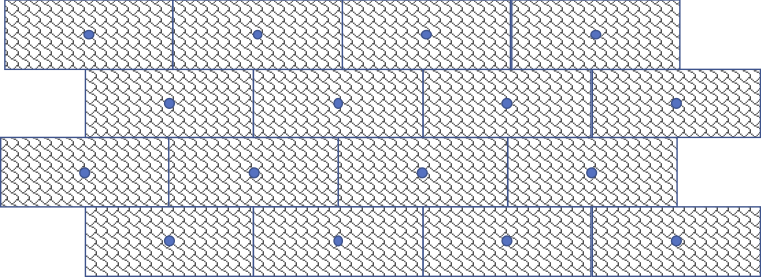
\includegraphics[width=0.6\linewidth]{figures/Bricks.png}
    \caption{A 2-D lattice generated from bricks. As a guide for equivalent points, a dot has been placed at the center of each brick.}
    \label{fig:latt1}
\end{figure}
  The problem with the cell to the left (in red) is that it is oblique – the angles between sides are not right angles – and thus we have lost some essential symmetry information about the rectangular bricks. The problem with the cell at the right (in green) is that while it preserves the rectangular symmetry of the bricks, it is twice as large as a single brick and thus is less than optimal in providing the simplest possible description of the lattice. Note that we cannot use a single brick as a unit cell, because that would violate the principle that a unit cell translation of applied to a point in any direction provides an identical point. Translation vertically by one unit would take a point from the middle of one unit cell to the edge of another. 
\begin{figure}
    \centering
    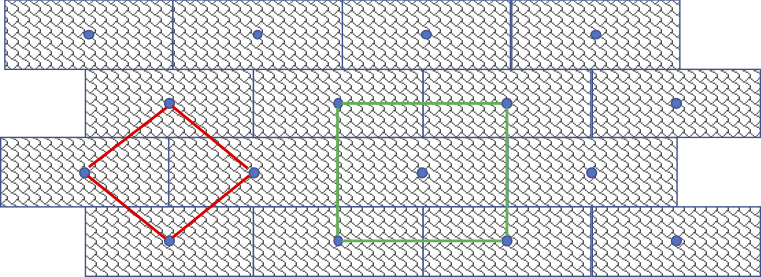
\includegraphics[width=0.6\linewidth]{figures/Bricks2.png}
    \caption{Two different unit cells, that will create the pattern in previous figure. The one in read does not show that the lattice symmetry is rectangular (orthorhombic).}
    \label{fig:latt2}
\end{figure}
 Lattice centering provides a secondary rule for lattice generation which places lattice points not only at the corners of unit cells but also at locations within cells. If we label axes above so that we are looking at the x-y plane and call the corners of the green box as (0,0,0), (1,0,0), (0,1,0) and (1,1,0) then we can also label the central point between them as (½, ½, 0). We already have said that adding any number of unit cell translations brings us to a point that is equivalent to our original point, which we can write algebraically as saying that point (x,y,z) is equivalent to (x+n\textsubscript{x},y+n\textsubscript{y},z+n\textsubscript{z}), where n\textsubscript{x}, n\textsubscript{y}, n\textsubscript{z} and n\textsubscript{c} can each be any integer. To express the idea that the environment of (½, ½, 0) is the same as (0, 0, 0) we can write an additional equivalence, that point (x,y,z) is equivalent to (x+n\textsubscript{x}+½ , y+n\textsubscript{y}+½, z+n\textsubscript{z}), where again n\textsubscript{x}, n\textsubscript{y}, n\textsubscript{z} and n\textsubscript{c} can each be any integer. 

 This brings us to the concept of a \textbf{symmetry operation},\index{symmetry operation} which will be needed when we discuss space groups. We use these only to describe the symmetry within the unit cell, so we do not need to consider the translations above, where we added integers to x, y or z as that relates the contents of one unit cell to a neighbor. However, one requirement of mathematical groups is that they must contain an identity operator, so even if there is pattern of repetition within the cell, the identity symmetry operation x,y,z must be present. However, in the case of the centering operation with our bricks, we can write a symmetry operator ½+x,½+y,z meaning that if we place an atom at coordinates (x,y,z), we automatically generate another a half unit cell away in both x and y. Note that if x>1/2 then x+½ will be in the next unit cell, but we can add or subtract any integer from x to translate back into the current unit cell, so ½+x+n\textsubscript{x},½+y,z is implied by ½+x,½+y,z and thus is equivalent to x-½,½+y,z.

 Lattice centering is most useful for crystal classes where the centered lattice demonstrates some symmetry that the \textbf{primitive lattice}\index{primitive lattice} (as we call a same lattice without centering) does not. If we place a lattice center into the middle of a triclinic cell, with coordinates (½, ½, ½) or equivalently consider this as the symmetry operation ½+x, ½+y, ½+z, it will have a doubled volume in comparison to any of the smallest possible primitive cells, but provides no extra symmetry information. This does not mean that it is illegal to use a centered description with a triclinic unit cell, in fact it may be useful for understanding what is changing when a material transforms from a structure with a centered cell to one that is triclinic, but the standard descriptions will not include any centered triclinic cells. In contrast, if we take an orthorhombic cell with a body center, we can construct several primitive cells, but none will have the three perpendicular axes found in the centered cell. Thus, centering allows us to demonstrate the full symmetry of that orthorhombic lattice. 

 There are two types of centers needed to construct the possible symmetry types for all three-dimensional lattices, known as the Bravais lattices\index{Bravais lattice}. One center type is placed in the side of a unit cell and called a face center. A face center with coordinates (½, ½, 0) is in the face perpendicular to \textit{c} and is called a C-center. Likewise, centers at (½, 0, ½) and (0, ½, ½) are called B-center and A-centers, respectively. As we saw before, a center at the middle of the unit cell is called a body center or is abbreviated as an I-center (short for the German word \textit{Innenzentriert}.). Combinations of centers are possible, but the only combination that cannot be simplified without loss of the underlying symmetry is when A-, B- and C-centers are \textit{all} combined. This combination is referred to as face centering or an F-center. Note that a A-, B-, C- or I-center will double the number of symmetry operations while face centering leads to four symmetry operations x,y,z; ½+x,½+y,z; ½+x,y,½+z; and x,½+y,½+z. Sometimes the expanded volume of a centered lattice is referenced by comparison to the low-symmetry primitive unit cell. Thus, a A-, B-, C- and I-centered lattice is doubly-primitive, meaning the centered cell has double the volume of the primitive cell. An F-centered lattice is quadruply-primitive. It is also possible to consider a lattice center on an edge of a unit cell, such as (½,0,0). Edge centers are used for description of unit cells for magnetic scattering but are not needed for the 14 Bravais lattices. 

 There is one special case of centering specific to related to rhombohedric unit cells. It is possible to transform any lattice constructed from rhombohedric unit cells (a=b=c, α=β=γ) into one that has a=b, γ=120° and α=β=90° unit cells,e.g. the same cell as a hexagonal lattice but this cell has three times the volume of the primitive rhombohedric unit cell and with lattice centers at (2⁄3, 1⁄3, 1⁄3) and (1⁄3, 2⁄3, 2⁄3). We use the symbol R is used for this type of centering. While both types of unit cells are used for this system because the same lattice can be generated either from a primitive rhombohedron or a triply-primitive centered cell in a hexagonal lattice, the hexagonal description tends to be used more commonly because it is usually somewhat more computationally simple.

\begin{table}
\centering
\caption{The 14 Bravais lattices as distributed across the 7 crystal systems, where P indicates a primitive cell, F for centers on all faces, I for a body center, R for rhombohedral centering (see text) and C for a C-center. Note that face centers can be interchanged between A, B and C-centering by relabeling axes.}
\begin{tabular}{| l | p{0.13\textwidth} | p{0.3\textwidth} | p{0.23\textwidth} |}
\hline
Name & Constraints on lengths & Constraints on angles & Bravais lattice centering options \\
\hline
Cubic & \textit{a}=\textit{b}=\textit{c} & α = β = γ = 90° & P, F, I \\
\hline
Tetragonal & \textit{a}=\textit{b} & α = β = γ = 90° & P, I \\
\hline
Orthorhombic & none & α = β = γ = 90° & P, C, F, I \\
\hline
Hexagonal & \textit{a}=\textit{b} & γ = 120°; α = β = 90° & P \\
\hline
Rhombohedral & \textit{a}=\textit{b}=\textit{c} & α = β = γ & R \\
\hline
Monoclinic & none & b unique: α = γ = 90° & P, C \\
\hline
Triclinic & none & none & P \\
\hline

\end{tabular}

\end{table}


\section{Crystallographic Symmetry Elements}

 So far, we have not considered where atoms are located within the unit cell, but it should come as no surprise that symmetry plays a role in that, too. If you have studied point group symmetry and not crystallographic symmetry, you have learned about two types of symmetry axes, proper and improper rotation axes, which are defined slightly differently in crystallographic use. However, point group symmetry does not include two additional types of symmetry that involve translations: screw axes and glide planes. Before reviewing these four types of symmetry elements, let’s dive deeper into the notation used to describe symmetry operations and their algebra. We use the concept of an operator to describe how a duplicate atom is created from the initial position with a triplet of formulae, \textit{f}\textsubscript{x},\textit{f}\textsubscript{y,}\textit{f}\textsubscript{z}, where each of the \textit{f}\textsubscript{i} is an algebraic expression dependent on x, y \& z. 

 As we saw, if we take an atom at position x,y,z and we have a body center in that lattice, this means that for every atom in the unit cell, there is another identical atom displaced from that atom by a half unit cell in each direction. We can write that as an operator as ½+x,½+y,½+z. We understand this operator to mean that we create a new atom from the first with its coordinates shifted by half unit cell translations. If the coordinates of the original atom is x,y,z and the coordinates of the second atom are x’,y’,z’, then x’=½+x, y’=½+y, z’=½+z. Likewise if we consider another symmetry operator, ½+y,-x,z, then that creates a copy of that atom where x’= ½+y and y’=-x but z’=z. 

 Symmetry can also be written as a matrix and vector. In this notation ½+y,-x,z would be written as 
 
$$\begin{matrix}x\prime\\y\prime\\z\prime\end{matrix}=\ \left[\begin{matrix}0&1&0\\-1&0&0\\0&0&1\end{matrix}\right]\left[\begin{matrix}x\\y\\z\end{matrix}\right]+\left[\begin{matrix}{1/2}\\0\\0\end{matrix}\right]$$

Let’s now consider a mirror plane symmetry operation, where we will place that symmetry element in the x,y-plane and at z=½. What does that mirror plane do? Viewed along the \textit{c} direction, perpendicular to the mirror plane, it appears to do nothing, because x and y will be unchanged by the action of the mirror plane. So, we can see the new position has the same values of x and y. Viewed from a direction in the plane of the mirror (for example, viewing along \textit{a} or \textit{b}), it becomes clear that the mirror plane involves a change in the z value to z’. A bit of thought makes clear that whatever the distance from the atom to the mirror plane, that distance must stay the same, but the atom will lie on the opposite side of the mirror plane. So, if our atom is at position z, then the distance to the mirror plane is |½-z| and the direction from the atom to the mirror plane will be along a vector from z to ½. For simplicity in visualization, we will assume 0 < z < ½, but what here is true for all values of z, assuming that a periodic lattice is present, so that adding or subtracting any multiple of one from z yields an indistinguishable value. The position on the other side of the mirror plane with the same distance to the mirror plane will be z’ = 1-z. We can see that |½-(1-z)| which is equal to |z-½|. Thus, we can say that our mirror plane in the x,y-plane and at z=½ is equivalent to a x,y,1-z operation. Since we can add or subtract any multiple of one to x, y and/or z, a simpler form for this operator is x,y,-z. Crystallographers have an even more compact notation for this, written as $x,y,\bar{z}$, where the last term is called “z bar” and means -z. Modern software does not make $\bar{z}$ easy to type, so I will use this notation sparingly.

There are two things we can learn from this x,y,-z operator. One is the idea of \textbf{special positions}, which is demonstrated by what happens if we have an atom that is placed on the mirror plane, meaning that that z=½ (note that x \& y are arbitrary). We can designate this in a more compact notation, as position (x,y,½). Applying this x,y,-z operator to position (x,y,½) generates position (x,y,-½). Since adding any positive or negative multiple of 1 to any coordinate generates an equivalent position in the lattice, the positions (x,y,½) and (x,y,-½) are indistinguishable and thus while in general an atom placed at (x,y,z) generates a second atom at (x,y,-z), the position (x,y,½) is special; we do not actually generate a new position for any atom with z=½. Thus, we say that due to the presence of this mirror plane, atoms at (x,y,½) are at special positions, because if there are \textit{n} atoms on one side of the mirror plane, then the mirror plane will generate a second set of \textit{n} atoms on the other side of the mirror plane and thus the unit cell must contain 2\textit{n} atoms, but not so for the atoms on the special position (x,y,½) because there will no duplicates for the atoms that lie on the mirror plane. The unit cell contents will thus be A\textsubscript{2n}B\textsubscript{n} where the B atoms have z=½ [or as we will see where z=0, as (x,y,0) is also a special position.] 

The second concept is that the presence of symmetry operators in combination with each other and/or the lattice can create additional symmetry operations. To understand how one symmetry operation can modify another operation, note that -x,-y,-z is equivalent to replacing the expression for x’,y’ and z’ with those values multiplied by -1. If we combine the -x,-y,-z and x,y,z symmetry operations this yields the original symmetry operation -x,-y,-z. If we apply -x,-y,-z to symmetry operation -x,y,½+z we get x,-y,½+z [note that -1*(½-y) is y-½ but in an lattice adding 1 but the completely equivalent position, ½+z, is preferred by convention.] Let us consider what happens with a mirror plane in the x,y-plane placed at z=0. This will “reflect” any atom at position z to z’=-z. The operator form of this is also x,y,-z, which is also identical to the operator created by the mirror plane at z=½. Thus, the presence of a lattice and a mirror plane at z=½ (and at –½, 1+½,…) requires the presence of an additional set of mirror planes at z=…-2,-1,0,1,2,… Likewise, a mirror plane at z=0 cannot exist without a mirror plane at z=½.

Now let us review the four types of symmetry elements.

\subsection{Proper rotations} Proper rotations are defined relative to a line and by the fraction of a circle that is rotated. Thus, to fully describe a proper rotation, we need to specify a direction relative to the \textit{a}-, \textit{b}-, and \textit{c}-axes and a point that the axis travels through and finally the fraction of a circle for the rotation (example: a 3-fold axis along \textit{a} that passes through y=z=¼.) The only rotations that are possible in crystals are 1-fold, 2-fold, 3-fold, 4-fold and 6-fold and the Bravais lattice dictates which of these are allowed. Thus, an N-fold rotation produces rotations of 360°/N (2p/N radians). Not all proper rotation axes can be found in any given Laue class. For example, a triclinic cell is not compatible with any rotation axis other than 1-fold. A 4-fold rotation axis interchanges axes and thus requires a minimum of two equivalent length axes (cubic and tetragonal cells), while a 3-fold axis requires a rhombohedric or hexagonal cell. A 6-fold rotation axis can only exist in a hexagonal cell. The symbol used for a N-fold proper rotation axis is simply the number 2,3,4,6 (no symbol is needed for the 1-fold)

Table \ref{tab:proper} shows the coordinates for atom positions generated by a proper rotation axis along the c-axis passing through x=y=0. Note that a 1-fold rotation axis is simply the identity operation. It generates only the original position of an atom. 
 
\begin{table}
\centering
\caption{Positions generated by a \textit{n}-fold proper rotation axis parallel to \textit{c} and passing through x=y=0}
\label{tab:proper}
\begin{tabular}{| p{0.1\textwidth} | p{0.075\textwidth} | l | l | l | l | l | l |}
\hline
Axis type & symbol & \multicolumn{6}{l|}{Generated atom positions} \\
\hline
1-fold &   & (x,y,z)  &   &   &   &   &   \\
\hline
2-fold & \textbf{2} & (x,y,z) & (-x,-y,z) &   &   &   &   \\
\hline
3-fold & \textbf{3} & (x,y,z) & (-y,x-y,z) & (y-x,-x,z) &   &   &   \\
\hline
4-fold & \textbf{4} & (x,y,z) & (-y,x,z) & (-x,-y,z) & (y,-x,z) &   &   \\
\hline
6-fold & \textbf{6} & (x,y,z) & (x-y,x,z) & (y,y-x,z) & (-x,-y,z) & (y-x,-x,z) & (-y,x-y,z) \\
\hline

\end{tabular}

\end{table}

\subsection{Improper rotations} Proper rotations are defined relative to a line for the rotation axis, but also a point along that axis. Thus, to fully define an improper rotation axis one needs the rotation order, a point and an axis of rotation. The way that improper rotations are applied is to first perform an inversion operation through the defined point and then apply the rotation, as was done with proper rotations. (Note that improper rotations, as used in molecular point group symmetry, are defined slightly differently and the Schoenflies labels work slightly differently; the crystallographic conventions are, of course, better.) Again, the improper rotation axes are named by the fraction of a circle that is rotated and again, only the only improper rotations that are possible are 1-fold, 2-fold, 3-fold, 4-fold and 6-fold, where only some of these are consistent with each Bravais lattice. Below is a table showing the coordinates for atom positions generated by an improper rotation axis along the c-axis and point x=y=z=0. The symbol used for a N-fold improper rotation axis is simply the number with a horizontal line above, as seen in the table. Note that the $\bar{1}$ operation is simply an inversion center, also sometimes called a center of symmetry. This does not have an axial direction, but does have an origin location. The $\bar{2}$ operation is simply a mirror plane. This is defined relative to a plane, but has no origin. Table \ref{tab:improper} shows the coordinates for atom positions generated by an improper rotation axis along the c-axis passing through x=y=0.

\begin{table}
\centering
\caption{Positions generated by a \textit{n}-fold improper rotation axis parallel to \textit{c} and passing through x=y=0}
\label{tab:improper}

\begin{tabular}{|  p{0.08\textwidth} | p{0.08\textwidth} | l | l | l | l | l | l |}
\hline
Axis type & symbol & \multicolumn{6}{l|}{Generated atom positions} \\
\hline
1-fold & \vspace{0.01mm}$\bar{1}$ & (-x,-y,-z)  &   &   &   &   &   \\
\hline
2-fold & \vspace{0.01mm}$\bar{2}$ & (x,y,z) & (x,y,-z) &   &   &   &   \\
\hline
3-fold & \vspace{0.01mm}$\bar{3}$ & (x,y,z) & (x-y,x,-z) & (-y,x-y,z) & (-x,-y,-z) & (y,y-x,-z) & (-y,x-y,z) \\
\hline
4-fold & \vspace{0.01mm}$\bar{4}$ & (x,y,z) & (-y,x,-z) & (-x,-y,z) & (y,-x,-z) &   &   \\
\hline
6-fold & \vspace{0.01mm}$\bar{6}$ & (x,y,z) & (y-x,-x,z) & (-y,x-y,z) & (x,y,-z) & (y-x,-x,-z) & (-y,x-y,-z) \\
\hline

\end{tabular}

\end{table}

\subsection{Screw axes} 
So far, we have seen point symmetry in the form of proper and improper rotations and the only translational symmetry we have seen is in the form of unit cell translations. There is also a symmetry operation that combines both rotational symmetry and translation. These are called screw axes and these describe helictical symmetry in a material. A screw axis has a defined translation direction and a location in the plane perpendicular to that direction. A screw axis is labeled N\textsubscript{m} where the first number, N, (2, 3, 4 and 6) describes the amount of the rotation, where the rotation is 360°/N (2p/N radians) so a 2\textsubscript{1} screw axis will cause a 180° rotation (generating 2 positions), while a 6\textsubscript{m }screw axis will have 60° rotations. The second number, m combined with N (the first), dictates the translation amount as m/N, so the translation is a half unit cell for a 2\textsubscript{1 }screw axis and one-sixth of a unit cell for a 6\textsubscript{1 }screw axis. Thus, a 2\textsubscript{1}screw axis will duplicate an atom (two atoms/cell) and a 6\textsubscript{1 }screw axis will create five copies (six atoms/cell). The crystallographically defined screw axes are 2\textsubscript{1}, 3\textsubscript{1}, 3\textsubscript{2}, 4\textsubscript{1}, 4\textsubscript{2}, 4\textsubscript{3}, 6\textsubscript{1}, 6\textsubscript{2}, 6\textsubscript{3}, 6\textsubscript{4} and 6\textsubscript{5}. Screw axes can occur along the \textit{a}, \textit{b} or \textit{c} directions or in three-fold symmetry materials (cubic and rhombohedric cells, along the body-diagonal, the 111 direction.) Thus, a full description of a screw axis will specify the type, the direction and a location of the axis, usually by giving a point that the axis travels through. 

 For an example, let us consider a 4\textsubscript{1} screw axis along the \textit{c} axis through the point x=y=0. The rotation portion of the axis will transform the in-plane coordinates of the atom from (x,y) to (-y,x) and then to (-x,-y) and finally to (y,-x) while simultaneously adding a ¼ unit cell translation. Thus, if we have an atom at coordinates (x,y,z) the generated positions are (-y,x,z+¼), (-x,-y,z+½) and (y,-x,z+¾).

 Note that since unit cell translations are applied in combination with screw axes, the translation of 5/6\textsuperscript{th} of a unit cell is the same as a translation of 1/6\textsuperscript{th} of a unit cell in the negative direction, thus a 6\textsubscript{1} and 6\textsubscript{5 }screw axes are an enantiomeric pair, that differ only in the rotation direction, where the 6\textsubscript{1} screw axis produces a right-handed helix and 6\textsubscript{5 }screw axis produces a left-handed helix. (The same is true for 3\textsubscript{1}/3\textsubscript{2}, 4\textsubscript{1}/4\textsubscript{3,} and 6\textsubscript{2}/6\textsubscript{4}.) Thus, the 4\textsubscript{3 }screw axis describes a helix with the opposite rotation direction of the 4\textsubscript{1} axis shown before, with generated coordinates (x,y,z), (y,-x,z+¼), (-x,-y,z+½) and (-y,x,z+¾). Note that while a 4\textsubscript{1} and a 4\textsubscript{3} axes will be found in different space groups, with powder diffraction all the reflections that could be sensitive to this rotation direction (due to anomalous dispersion) are superimposed, so it is impossible for a powder diffraction experiment to differentiate the enantiomeric handedness for a material. Without some other type of data, the distinction between each pair of related symmetry elements can be ignored. Space group \textit{P}6\textsubscript{1} and \textit{P}6\textsubscript{5} are considered different space groups as they can accommodate objects of with different handedness, but to powder diffraction they are the same. 

\subsection{Glide planes} The last type of symmetry element found in crystals combines translation and reflection and is called a glide plane. A glide plane causes an atom to be translated by a half-unit cell in one direction and then reflected through a plane. We name the glide plane for the translation direction (as an a-glide, b-glide or c-glide), but the full description for a glide plane will also name the reflection plane by specifying the perpendicular axis (which obviously must be a different axis than the translation direction.) If we take for example a c-glide perpendicular to \textit{a}, which I placed at x=0, we can see that the reflection operation will take (x,y) and transform that to (-x,y) the translation of a half-unit cell adds to z. Thus, coordinates (x,y,z) are transformed to (-x,y,z+1/2).

There are few special types of glide planes. An \textit{n}-glide, which is sometimes called a diagonal glide, is similar to a a-glide, b-glide or c-glide except that the translation is applied along two axes and the glide is named for the axis normal to the reflection plane. One must specify the coordinate along this axis to know where te . As an example, in space group \textit{Pn} there is a n-glide perpendicular to \textit{b} at y=0. This will cause an atom to be reflected from y to -y followed by a translation along both a and c, thus the operator for this will be ½+x, -y, ½+z. 

 A \textit{d}-glide, sometimes called a diamond glide, involves a reflection followed by a translation along either a face-diagonal direction (translating along a+b, or a+c, or b+c, or any positive or negative permutation, such as a-b, -a-b or -a+b) or a body-diagonal direction (which can be any of the 6 directions permuting +a, -a, +b, -b and +c,-c). However, the translations for a d-glide is a quarter of a unit cell unlike all other glide plane types. Note that d-glides are only found in body-centered (I) and face-centered (F) lattices. A specify a d-glide, one needs to indicate the direction of the translation as well as the location and orientation of the reflection plane. As an example, a d-glide along the 110 diagonal and perpendicular to \textit{c} at z=0 will have operator ¼+x,¼+y,-z. 

\section{Space groups}

The mathematical concept of a group is a bit different from the sort of practical math that is most commonly taught, such as algebra, trigonometry and calculus, but one of the great discoveries (of the 18\textsuperscript{th} century) when it comes to describing the possible types of symmetry that can be found in isolated objects (point groups) or objects in a lattice (\textbf{space groups}). Returning to the operators For our purposes, we can consider these operations as the symmetry actions that will determine the positions of atoms in our unit cell. 

Groups are built from operators, which for our purposes we will consider as giving us the coordinates for duplicate copies of atoms at other locations, as we saw before. To give this important mathematical concept a very brief overview, the key mathematical requirements of a group are that every group must have an identity operation and that group must be complete, meaning that any operator in the group if performed on another operator in a group will generate an operator that is also contained in the group. This means that all permutations of each operator combined generates an operator in the group. This also requires that there must be an inverse operator for every operator in the group.

 We will write the \textbf{identity operation }as x,y,z, meaning that an atom with coordinates (x,y,z) is placed at those coordinates. The simplest group has only this operation and we can see that this group is complete, meaning that any repeated set of operators from the group, in any order, will only create another operator in the group. Thus, a single operator, x,y,z, creates our simplest group, since x,y,z operated on x,y,z gives us the original operator back. This, combined with a translation operators from an infinite lattice, is labeled by crystallographers as \textit{P }1 using what is known as the Hermann-Mauguin space group notation. 

 If we consider the mirror plane operator we saw before, x,y,-z, and combine that with x,y,z, we create a second group with just two elements, since x,y,-z operated on itself gives x,y,z and x,y,-z operated on x,y,z gives back x,y,-z. Combined with a lattice, these two operators will generate a space group \textit{P m} using short-form Hermann-Mauguin notation (or \textit{P }1 1 \textit{m} in long-form Hermann-Mauguin notation, where the 1 indicates there is no symmetry along the \textit{a}or \textit{b} axes.) Some head-scratching about mirror planes will show that a lattice must have an axis that is at right angle to the mirror plane (if not lattice points will not be reproduced at the correct positions), so \textit{P m} is only consistent with a monoclinic unit cell. When I say only consistent with monoclinic, this does not preclude a unit cell that appears to be of higher symmetry, for example it could have all three cell axes appear as 90° within arbitrarily small experimental errors, but only one of these angles is constrained by symmetry to be 90° and thus the cell would not be considered to be orthorhombic unless additional symmetry is present that requires all angles to be 90°.

 We can also take the \textit{P m} space group and add an additional centering operation to create a new space group. Let’s add a B-center which means operator ½+x,y,½+z. When this is operated on x,y,-z we create fourth additional operator, ½+x,y,½-z. Using these four operators on each other, we generate no others. Thus, the space group \textit{B }1 1 \textit{m} has four operators: x,y,z; x,y,-z; ½+x,y,½+z; and ½+x,y,½-z. Note that we used only two symmetry operations (the mirror plane and centering) to generate these four operators. We call those two operators the \textbf{generators} because those two operators can be used generate the entire group and those generators are thus included in the Hermann-Mauguin name. It is also worth noting that Volume A of the \textit{International Tables for Crystallography} does not include \textit{B} 1 1 \textit{m} as one of the 230 space groups, but a closer look at the volume one can find \textit{B }1 1 \textit{m} as one of the non-standard settings for space group \textit{A }1 \textit{m }1. 
 The 230 three dimensional unique space groups tabulated in the \textit{International Tables for Crystallography, Volume A} only reflects only the standard settings for space groups. 
 Just as the \textit{International Tables }lists \textit{B}\ 1\ 1\ \textit{m} as one of the non-standard settings for space group \textit{A}\ 1 \textit{m}\ 1, one could also consider F centering or I centering with a mirror plane and generate other versions of space groups. 
 There are a large number of non-standard space groups. 
 These can always be reduced or transformed to one of the 230 standard space groups, but there can be good reasons why use of a non-standard space group can be very convenient, most commonly because it allows direct comparison of coordinates between related structures. 
 As we will see, GSAS-II does allow you to use these non-standard settings, and they can be quite useful. 

 We saw before that the combination of operations -x,-y,-z and -x,y,½+z generates x,-y,½+z. Thus, we know that -x,-y,-z and -x,y,½+z alone cannot form a group, but you can convince yourself that the four operators, x,y,z, -x,-y,-z, -x,y,½+z and x,-y,½+z do constitute a group. 

 When considering classes of space groups, one must consider that a hexagonal cell can host a structure with a 6-fold (or $\bar{6}$) rotation axis or a 3-fold (or $\bar{3}$). The later are considered trigonal space groups and the former hexagonal. Since rhombohedral symmetry can also be expressed in a hexagonal cell, they are labeled as a special centered case within the trigonal space groups and are given an R prefix. 

\section{Systematic Extinctions}

An important consideration of symmetry is that translational symmetry, where atoms are offset from their original positions by a fixed amount, will cause classes of reflections to have zero intensity, known as systematic extinctions or systematic absences. Only translational symmetry operations (cell centering, screw axes and glide planes) can cause systematic extinctions, while the presence of proper and improper rotation operations do not cause systematic extinctions except in combination with translational symmetry. 

To understand how systematic extinctions arise, let us consider a unit cell with a C-center. To simplify we will assume that the unit cell has only two atoms, if the first is at x,y,z then the second will be at x+1/2, y+1/2, z. If take the structure factor equation, 

$$F_{hkl}=\sum_j^N f_j \exp⁡[-2πi(hx_j + ky_j + lz_j)]$$

and expand this over our two atoms, we get 

$$F_{hkl} = f_j \exp⁡[-2πi(hx_j + ky_j + lz_j)] f_j + \exp⁡[-2πi(hx_j + ky_j + lz_j) + \frac{h+k}{2}] $$

which can be rewritten as 

$$ F_{hkl} = f_j \exp⁡[-2πi(hx_j + ky_j + lz_j)] f_j + \exp⁡[-πi(h + k)] \exp⁡[-2πi(hx_j + ky_j + lz_j) ] $$

Note that when h + k is even, then $\exp⁡[-πi(h + k)] = 1$ but when h + k is odd then $\exp⁡[-πi(h + k)] = -1$ so the sum of the two exponentials is zero. Thus, for C-centering with any number of atoms in the unit cell,  $F_{hkl}=2\sum_j^{N/2} f_j \exp⁡[-2πi(hx_j + ky_j + lz_j)]$ for h+k even, and $F_{hkl}=0$ for h + k odd. 

We can also rationalize this by thinking that if viewed along a reciprocal space direction, symmetry causes the unit cell repeat distance to decrease by a half, then half of the reflections in that projection must disappear. For a 2\textsubscript{1} screw axis along \textit{a}, the viewed along the \textit{a*}-axis, the cell will appear to be half the original size. Thus, \textit{h}00 reflections will be absent when \textit{h} is odd. This only occurs in projection along \textit{a*}. From any other direction this superposition is broken. Likewise, for a \textit{c}-glide plane perpendicular to the \textit{b}-axis, this appears to halve the c-axis length except when not perpendicular to \textit{b}*, so \textit{h}0\textit{l} reflections must have zero intensity when \textit{l} is odd.

 \section{Site symmetry and the asymmetric unit}\label{ref:asymmetricunit}
As noted before, some space groups have locations where if an atom is placed, some symmetry operations will generate the same position again rather than a different location. These are called special positions, which may be a point, line or even plane. For every space group, the \textit{International Tables} has a tabulation of special positions known as the Wyckoff sites. These consist of a number followed by a letter. The number indicates the number of these type of positions that occur in the cell, which is known as the multiplicity. The letter is assigned sequentially. The first item, will have the largest multiplicity, and the last assigned letter will be the the lowest symmetry locations in the cell and with it will be listed the equivalent locations. The subsequent Wyckoff sites will have higher symmetry and lower multiplicity and the locations where that occurs. If a line, it will be expressed as a formula such as (x,0,0) or (x,x,0) and if a plane (x,y,0). 
As an example, the space group $P 2_1/c$ has the following Wyckoff sites listed:

\begin{itemize}
    \item 4e:  $(x, y, z)$; $(\bar{x}, y+\frac{1}{2}, \bar{z}+\frac{1}{2})$; $(\bar{x}, \bar{y}, \bar{z})$; $(x, \bar{y}+\frac{1}{2}, z+\frac{1}{2})$
    \item 2d: $(\frac{1}{2}, 0, \frac{1}{2})$; $(\frac{1}{2}, \frac{1}{2}, 0)$
    \item 2c: $(0, 0, \frac{1}{2})$; $(0, \frac{1}{2}, 0)$
    \item 2b: $(\frac{1}{2}, 0, 0)$; $(\frac{1}{2}, \frac{1}{2}, \frac{1}{2})$
    \item 2a: $(0, 0, 0)$; $(0, \frac{1}{2}, \frac{1}{2})$ 
\end{itemize}
The 4e Wyckoff site is the general position and the other four Wyckoff sites are pairs of discrete points in the unit cell. Alas, the listing order of Wyckoff sites, other than in decreasing multiplicity, is not in any derivable sequence and thus is only a reference to the \textit{International Tables} tabulations. I tend to avoid use of Wyckoff labels as I consider the letter assignment to be arbitrary. 

Related to site multiplicities is the concept of the asymmetric unit. This can be expressed in two different ways. The \textit{International Tables} lists an asymmetric unit for each space group as a unique volume within the unit cell and if that unique volume is duplicated using the symmetry operators, the entire contents of the unit cell can be constructed. The other way that the asymmetric unit is described is in terms of the unique atoms that can be used to build up the unit cell contents. Note that each atom in the asymmetric unit will then have a multiplicity. The previous expression for the structure factor can then have the number of terms reduced

$$F_{hkl}=\sum_j^{N^\prime} f_j m_j\exp⁡[-2πi(hx_j + ky_j + lz_j)] \exp⁡[-2πi(\vec{Q}\cdot\vec{U_j})]$$

where the summation over $N^\prime$ reduced to a summation over the number of atoms in the asymmetric unit rather than the entire unit cell contents and an extra term, $m_j$, is included for the multiplicity of each atom site. 

\section{Space groups in GSAS-II}

In GSAS-II, to simplify the listings of the symmetry operations, they are shown in a manner that minimizes the number of operators that must be provided. This is done by providing only the unique operators, if there is a center of symmetry and lists the centering operations. The full set of operations will be created by applying the center of symmetry and centering operations to the unique operators. An example will show how this works. For the space group, \textit{F }2/\textit{c} (which is a non-standard setting of the monoclinic space group \textit{P }2/\textit{c}) there are 16 symmetry operations, 
\begin{center}
x,y,z \\
-x,y, ½-z \\
-x,-y,-z\\
x,-y,z+½\\
x,y+½,z+½\\
-x,y+½,-z\\
-x,½-y,½-z\\
x,½-y,z\\
x+½,y,z+½\\
½-x,y,-z\\
½-x,-y,½-z\\
x+½,-y,z\\
x+½,y+½,z\\
½-x,y+½,½-z\\
½-x,½-y,-z\\
x+½,½-y,z+½
\end{center}

GSAS-II displays the window in Fig. \ref{fig:F2_c}
for this space group.

\begin{figure}
    \centering
    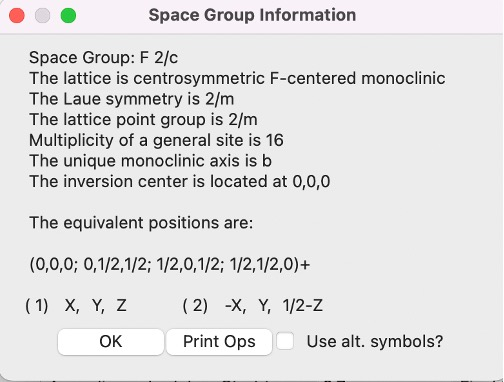
\includegraphics[width=0.5\linewidth]{figures/F2_c.jpg}
    \caption{Information displayed by GSAS-II for the non-standard space group $F 2/c$}
    \label{fig:F2_c}
\end{figure}
Note that at the bottom of this window, two unique symmetry operations are given: x,y,z and -x,y,½-z, but as noted the multiplicity of a general site is 16, meaning there must be a total of 16 symmetry operations. The two initially supplied symmetry operations are doubled because this space group is noted as centrosymmetric. Thus, the center of symmetry operation, -x,-y,-z, is applied to each of the two initial symmetry operations, generating two additional operations, -x,-y,-z and x,-y, ½+z. These four symmetry operations are also operated upon by the four centering operations, listed as (0,0,0)+, (0,½,½)+, (½,0,½)+, (½,½,0)+. The first centering operation gives us back the four operators already listed, but adding (0,½,½) to each of these the four operators we already have provides us with four new operations: x,½+y,½+z, -x,½+y,-z, -x,½-y,½-z and x,½-y,z. Likewise, applying the (½,0,½)+, (½,½,0)+ operations will generate the other 8 symmetry operations. Thus, we generate all 16 of the operators listed above. Pressing the “Print Ops” button causes these 16 operations to be displayed in the GSAS-II console window. 

The use of these grouped operators allows the most complex space groups (which have 192 operators) to be shown in GSAS-II with only 24 basic operators, where these 24 operators will be doubled to 48 by a center of symmetry, and then each of the three additional centering operators will provide another 48 operators giving us a total of 192 (=24*2*4).

 Space groups are input to GSAS-II with a space between each set of symmetry operations, so the space group \textit{P}6\textsubscript{3}/\textit{mmc} will be specified as \texttt{P 63/m m c}, though for standard settings, space group symbols will be recognized even if the spaces have not been specified correctly. 

One place where GSAS-II is quite restrictive is with centrosymmetric space groups where the highest symmetry location in the cell is not a center of symmetry. Such space groups are documented in the \textit{International Tables} with two choices for origin. In the first origin setting ("Origin 1")\index{Origin 1}, the highest symmetry position is selected as (0,0,0), while Origin 2\index{Origin 2} places a center of symmetry at (0,0,0). Origin 2 is computationally much simpler (since reflection phases are real). GSAS-II only accepts structures in Origin 2 settings in those space groups where there is a choice. When a structure is imported into GSAS-II where this choice exists, if symmetry operators are in the file (currently only in some CIFs), and an Origin 1 setting is detected, GSAS-II will perform the necessary translation to place the structure into Origin 2. Without symmetry operators, the origin can not be determined automatically, but atom multiplicities are computed using both origin settings and usually it is clear which origin setting will provide the correct stoichiometry. As a last resort, plotting of the structure will almost always make it very clear if a reasonable bonding geometry is being generated. If the origin setting is wrong, the generated diffraction pattern will also be wrong. 

Finally, in rhombohedral space groups, the cell is assumed to be hexagonal. To specify that the primitive rhombohedric cell should be used, add a final letter “r” to the space group name. Thus, “R 3” will provide symmetry for a hexagonal cell, but “R 3 r” will provide the symmetry for a rhombohedric cell. Usually, refinements are more stable with the hexagonal cell. 
\chapter{Powder Diffraction}
\label{Chap:powder}

Powder diffraction\index{powder diffraction} was invented by Peter Debye\index{Debye, P.} and Paul Scherrer\index{Scherrer, P.} , as well as independently by Albert Hull\index{Hull, A.} all in 1917, during World War I. 
Working in Germany, Scherrer and Debye were fortunate to be Swiss and (then) Dutch citizens, respectively, as this exempted them from being drafted. Hull worked for a U.S. Company, General Electric, which was a defense contractor.
Having also worked in U.S. companies, he has my sympathies, but I do note that Hull did go on to have several other important inventions. 
Powder diffraction was used initially for the purpose of descriptive crystal-structure determination, for materials where single-crystal specimens for materials were not available. 
It was also initially deployed because the powder diffraction pattern provided a unique structural "fingerprint" for materials.

The name powder diffraction is really a misnomer, as it is used for much more than measurements on powders. A better name for the technique would be polycrystalline diffraction, as it can be used on any sort of bulk material that has a large number of unoriented small crystal components. However, with more than 100 years of tradition behind us, I think it is too late to lobby for a different name. 

An ideal powder diffraction experiment has a large number (typically millions) of crystals that have random orientation. As we will see, powder diffraction is commonly used on samples where the crystal orientation is not completely random. The phenomenon when crystallite orientation ordering is not random is called preferred orientation\index{preferred orientation} and the description of how crystals are oriented is often referred to as texture\index{texture}. 
Powder diffraction is commonly used for the quantification of texture. 
In fact, it is also used for partly- and non-crystalline materials. 
We tend to use the term crystallite\index{crystallite} for each component crystal in a polycrystalline material, where a crystallite is the domain of atoms that all have the same crystallographic order. For metals, the term grain\index{grain} is used for exactly the same meaning as that of crystallite. 

It might be thought that a random orientation of crystallite would produce a random scattering of x-rays, electrons or neutrons, but this is not what happens because diffraction 

As we have seen, diffraction can only occur when the structure factor, $F_{hkl}$, is non-zero and this only occurs for discrete values of $h$, $k$ and $l$ and at specific Q values, where 

$$F_{hkl}=\sum_j^N f_j \exp⁡[-2πi(hx_j + ky_j + lz_j)]$$

Both groups and many others were successful in this work, but as the practice of single-crystal diffraction analysis improved, and structure refinement allowed quantitative structure determina- tion to become routine, one of the key weaknesses of powder diffraction – the loss of information due to reflection overlap – became a major disadvantage. In the relatively few cases where structural refinement from powder diffraction was attempted, reflections that overlapped had to be discarded. Alternately, refinement software was created to treat the specific cases of groups of overlapped reflections for each structural study [for example, see Rietveld (1966)].
\chapter{An Introduction to the GSAS-II GUI}
\label{Chap:GSASIIintro}

While this prerequisite chapter is a bit different from the previous, in that I do not expect that you will have previously seen the information here, I do think that having a familiarity with GSAS-II will be helpful before moving on to the rest of the book. In subsequent sections, I will frequently alternate between introducing concepts and then showing how those concepts are embodied when using GSAS-II. For this reason I want to provide an orientation for how GSAS-II is installed and organized here.

\section{Installing GSAS-II \& Web Resources}
GSAS-II is hosted on GitHub.com and is typically downloaded from there. All information related to GSAS-II is indexed via the GitHub home page, \texttt{https://GSASII.github.io}.\index{GSAS-II home page} Please refer to the section of that website (\texttt{https://advancedphotonsource.github.io/GSAS-II-tutorials/install.html}) which provides installation instructions\index{GSAS-II installation instructions}. Most people will choose to download one of the GSAS2MAIN self-installers, but there are many different ways that GSAS-II can be installed depending on your own preferences and goals. The installation instructions web pages provide a detailed  discussion of the options and advantages. It is worth noting that the source code for GSAS-II is installed as part of the GSAS-II installation, so we try to keep the size of that small. This source code is found in GitHub repository  \texttt{https://github.com/AdvancedPhotonSource/GSAS-II}, but there are three other repositories associated with GSAS-II. The GSAS-II documentation, including tutorial web pages, and input used to create  the web pages, help pages and newer tutorials is found at \texttt{https://github.com/AdvancedPhotonSource/GSAS-II-tutorials}. Routines used to compile and package GSAS-II, as well as the distribution files for installation are found in repo https://github.com/AdvancedPhotonSource/GSAS-II-buildtools and finally the files used to create this book are found at \texttt{https://github.com/briantoby/PowderCrystallography}. The GSAS-II code developer's manual, which is a formatted version of text and comments found in the source code is hosted on a separate site, \texttt{https://gsas-ii.readthedocs.io/}.\index{GSAS-II Developer's manual} The documentation section of the home page provides access to the manuals in several formats.  

\section{The GSAS-II GUI}
When initially started, GSAS-II uses three windows. As it is used it will commonly open  "modal" dialogs, which are additional, usually small, windows that "lock" the application until information is entered. It occasionally may open other windows, such as web pages, that work independently of the rest of the program and may persist until that window is closed. The three windows are, the main window, the graphics window and the console window, which will be discussed in the following sections. 
\subsection{The main GSAS-II window}

\subsection{The GSAS-II graphics window}
\subsection{The GSAS-II console window}


\part{Pattern Fitting}



\chapter{Overview: Fitting diffraction patterns}

There are four key aspects for obtaining a good fit to a powder diffraction pattern in a Rietveld refinement: 
\begin{itemize}
     
\item Fitting the background, which means reproducing the slowly-varying parts of the diffraction pattern, that arise from instrumental artifacts as well as non-Bragg scattering from the sample (Chapter \ref{Chap:background}),

\item Fitting the peak positions, which are determined by lattice parameters and instrumental calibration/corrections must be in the correct places
(Chapter \ref{Chap:peakpositions}).


\item Reproducing the peak intensities, as determined from the crystal structure model as well as corrections such as preferred orientation and extinction 
(Chapter \ref{Chap:intensities}).


\item Matching the shapes of the peaks, as this must reproduce the broadening effects of both the diffraction instrument and effects from the sample (Chapter \ref{Chap:profile}). 

\end{itemize}

Each of these aspects of fitting will be discussed in the following chapters. 

\chapter{Fitting Background}
\label{Chap:background}

The process of fitting the background in a diffraction pattern is potentially complex, in that GSAS-II provides four different computational mechanisms for background fitting and these are commonly used in combination. These will be described further, below. GSAS-II provides some unique tools can assist in background fitting. They are not needed for the simple cases, but may greatly simplify the problems associated with background modeling for the problem cases, where background is not a smooth slowly increasing or decreasing function.

The process of fitting a background is conceptually simple. Any scattering that is not Bragg scattering from the sample needs to be defined as part of the model used for fitting. The background model is added to the Bragg scattering to produce a simulation that reproduces the entire observed diffraction pattern. If the background is not well fit, it will degrade the overall fit and may cause parameters in the Bragg fitting to deviate from the correct values as the refinement attempts to minimize the differences between the observed and computed pattern. Most commonly, the parameters that would be affected by a poor background fit are the atomic displacement parameters ($\rm U_{iso}$) and/or peak shapes, but on occasion structural parameters can be biased. I should note that I am a firm believer that the final fits the background model should be optimized against the data rather than be fit by what the scientist thinks is correct. The best model predicted by the data is what is needed to minimize the overall fit while also obtaining chemically plausible results. While in the early stages of a fit, it may be best to fix the background to be in the locations that look right to our eye, my preference is that in the final stages, the profile be refined. There is one exception to this, which is when all the $\rm U_{iso}$ values refine to much lower than expected values. In this case it may be necessary to use a hybrid approach, as will be discussed in section \ref{negativeUiso} of this chapter.

Before discussing background fitting, I will define one term that is useful for these discussions, the baseline. I will speak of the baseline as function that describes the background as a function of TOF, $2\theta$, Q, etc. This is the average intensity well away from any Bragg peaks, but will be well below the data in the regions where peaks are found. Note that where noise levels are high, there may well be data points that are below the baseline, since the noise will scatter the data points around this average. Date may not return to the baseline for quite some distance from peaks, if the broadening has appreciable Lorentzian character (from sample broadening), since the Lorentzian line shape has very long peak tails. 

\section{Background Computation Modes}

The goal for a background fitting function is that it should produce a smoothly varying intensity curve over the range of $2\theta$ or TOF values and the complexity of the curve should depend on the number of terms for the 

GSAS-II provides several different background functions thapproaches for computing background scattering. 

\subsection{Smooth Refined Functions}

GSAS-II provides a number of functions that can be 

\subsection{Debye Scattering Peaks}

\subsection{Background Peaks}

\subsection{Fixed Background Histogram}


\section{Approaches to Fitting Background}

 Further, while sometimes all that is needed is to pick the right function and refine its coefficients, that does not always work, so GSAS-II provides both a manual and a semi-automated way to "bootstrap" the background. 

\subsection{Setting Data Limits}
One key step in background fitting is to use the right data limits for the refinement. It is common that the low Q portion of a diffraction pattern has a complex background. If there are no diffraction peaks in that region, one is only making the fitting process more difficult by including that portion of the pattern. Make sure to set the low Q data limit (low angle or long TOF time) so that the lowest-order observed diffraction peaks are included in the computation but do not include data at much lower Q than where the first peak reaches the baseline. While typically not a problem with respect to background fitting, including data at too high a Q value is also not a good idea. Look at the data at high Q and see if there are observable changes in intensity or if the intensities are too small to see relative to the noise level. Fitting noisy data can be helpful, but do not include data at high Q where there is only background to fit. The most important reason to not include this "flat"  data at high Q is not for background considerations, but due to the time needed to perform computations. As the range of the pattern increases in Q, the number of reflections increases by ~$\rm Q^3$ and the time needed to compute the pattern also increases on that order. This is most noticeable with TOF data, where a small change in the minimum TOF time can add a very large number of reflections to the pattern. I have seen least-squares refinement cycle times drop from minutes to seconds with the choice of sensible diffraction limits. 

Limits for the range of data to be used in fitting are stored on the Limits data tree entry and can be changed there, but can also be changed by dragging the green and red vertical dashed  lines from the plot for the background tree entry.

\subsection{Measuring Instrumental Background}

GSAS-II allows you to measure a diffraction pattern that will be subtracted from your observed pattern, point by point. Note that the two patterns must have the same point spacing and the same start and ending values. This can be a very useful thing, when working with "background-rich" data collection environments, common with \textit{in situ} experiments where ancillary equipment (furnaces, refrigerators/cryostats, reaction cells, etc.) can produce significant amounts of scattering that can have sharp features that are hard to reproduce. When I worked on PDF determination, where it was important to separate non-Bragg scattering from the sample from instrumental background, we collected the background scattering from the instrument without any samples and a pattern with the sample refrigerator but without any samples loaded, ideally with an empty sample container. One might think that simply subtracting the observed background that empty ancillary equipment should account for all background, but there are several issues that this will not address. The first is that the absorption and diffraction from the sample reduces the amount of radiation that can be scattered from the ancillary equipment. This means that the measured background will usually be a slight overestimate for what is actually observed from that source. In GSAS-II, one can specifiy 

\section{Negative $\rm U_{iso}$ values}\label{negativeUiso}
On occasion it is not possible to refine the peak shape, ADP’s (Uiso values) and background together. This is usually in materials that have many peaks, and where the peaks start to overlap so that beyond some value of Q there are no areas without reflections so the intensities are always above the baseline for a large region of the pattern. These areas without peaks define where the background must be located. This means that if the high-Q background were to be placed at a slightly lower level, a comparable fit can be obtained by increasing the intensity of the high-Q data (by lowering the Uiso values for the atoms) and adjusting the peak shapes to put more intensity into the peak tails. The symptom for this will be a refinement that seems quite good in quality, but has very low, often negative, U\textsubscript{iso} values. If a single U\textsubscript{iso} value is negative and all other atoms have expected values, this can mean that the atom type is wrong or the occupancy is too low and more scattering density is needed at that site, but when all U\textsubscript{iso} values are low this is an indication that there is not a single model to fit the data, but rather a range of values that produce similar fits. 

 My solution for this is to set all the U\textsubscript{iso} values to a value somewhat larger than I would expect based on my experience for the material type and data collection temperature and then fit the background and sample broadening. I then stop fitting the background but do fit the U\textsubscript{iso} values again. At this point the U\textsubscript{iso} values will typically refine to larger values. Do note in any publications that the background could not be refined in the presence of other parameters and needed to be fixed. 
\chapter{Fitting Peak Positions}
\label{Chap:peakpositions}

Intro to peak position fitting here
\chapter{Fitting Peak Intensities}
\label{Chap:intensities}

Intro to peak intensities fitting here
\chapter{Fitting Profile functions}
\label{Chap:profile}

As discussed before, to match the shapes of the peaks, you must reproduce the broadening effects of both the diffraction instrument and effects from the sample. 
What determines these broadening effects and how they are introduced into the fit will be the subject of this chapter. 

For some studies, determining the broadening characteristics is only needed as a means to obtain a good fit to the pattern, allowing determination of lattice or structural parameters, and indeed this was the original goal when Hugo Rietveld\index{Rietveld, H.} developed his eponymous analysis process. However, the parameter values that are used to model the peak profiles can provide information on the sample at the microscale, which can be very important for understanding the properties of a material that are not intrinsic to the substance but rather depend on how the substance was processed. Traditionally, microscopic techniques are well suited to provide the most detailed information on things like crystallite size and morphology, but Rietveld analysis has an advantage in that it provides measures that represent the entire sample bulk. Bulk characterization of a sample by microscopy is typically a very tedious process. The downside of sample characterization from powder diffraction is that it requires careful work to separate sample from instrumental effects.

 

\section{Peak broadening contributions convolute}

Before considering how broadening arises, it is worth mentioning that when multiple sources of broadening occur together, the each broadening contribution acts on each other in a process called convolution, which is reproduced mathematically by a convolution integral, a fairly slow computation. Use of a Fast Fourier Transform speeds this computation, because taking two functions, Fourier transforming them, multiplying the transforms together and then taking the inverse transform of the product is equivalent to performing a convolution integral, but even that is a fairly involved computation. 

 I like to think about broadening as an analogy to optical aberrations. Broadening is in effect a blurring of the peak position that comes from multiple compromises in the design of a diffraction instrument, as well as possible imperfections in the instrument, as well as defects in the sample. For those of you who, like me, must wear glasses to see well, we know that dirt on the lenses degrades our ability to see clearly. Bright sunlight, which allows the iris of our eye to become more like a pinhole camera, decreases the impact of this \textit{schmutz}. As an analogy for how broadening sources combine, consider what you see looking out a glass window. If the window glass is not uniform in thickness, then your view of the outside will be distorted where some aspects of the view will be enlarged, and others decreased in size since the window will act like a lens. If in addition, it is raining and the window is covered with rain, then the view will also be blurred, so your view of the outside will be both blurred and distorted. However, if the rain is heavy enough then the view will be so blurry that the distortions become hard to distinguish. A similar effect happens with broadening, where if we have two types of broadening that have relatively similar impact, then the two effects largely (but not exactly) add. If one broadening term is causing significant change to the signal and the other causes much less impact, then the convolution product will be only slightly changed from the more significant broadening source. 

 

\section{Sources of instrumental broadening}

So, what are the sources of instrumental broadening in powder diffraction? There are many, but let’s consider a few. First of all, how well is the wavelength determined for the probe? For conventional x-ray sources, there are usually several characteristic x-rays lines, typically labeled as Ka\textsubscript{1}, Kb, etc. These lines are fairly sharp with respect to wavelength spread, but most instruments do not isolate a single one of these lines and thus the diffraction pattern that is observed is actually a superposition from several different wavelengths. With synchrotrons and reactor-source neutrons, at least one (with synchrotrons usually a series of two or more) monochromator crystals must be used to isolate the intended radiation. A key design aspect in these instruments is how broad the wavelength range that is allowed through the monochromator, where synchrotron instruments usually transmit a very narrow portion of the radiation, with a great loss of intensity, while for reactors, the monochromator crystals are usually deformed in some fashion to transmit a much wider range of the radiation in order to retain much more of the neutron flux.

 With time-of-flight (TOF) neutrons we measure the wavelength by timing how long it takes for the neutrons to transverse the distance from the source to the detector. While a very sharp “flash” of neutrons is emitted when a pulse of protons hits a heavy metal target, these neutrons are very high energy and must be moderated by bouncing around in a material where they transfer some of their energy. Not all the neutrons will leave the moderator at the same time, and this results in a spread in the time of arrival for neutrons with the same energy. This delay effect is not symmetrical, so that TOF peaks are broadened more with neutrons arriving “late” than what would be seen if the probably for early arrival with respect to the mean time of flight were the same as late arrival. Further, since less energetic (slower) neutrons are likely to have bounced around in the moderator for longer than their higher-energy cousins, the time profile for when neutrons will arrive is narrower for higher energy (short wavelength) neutrons than for lower energy (long wavelength) neutrons; thus the resolution changes with wavelength.

 For both lab and user facilities, the spectrum of the x-rays or neutrons will never be perfectly sharp, so there is always some range in energy, which results in some broadening in diffraction peaks.

 A second contribution for aberration is the finite size of the radiation source. Remember that we need to measure the diffraction angle at infinite precision, if we want to see an infinitely sharp peak. If we do not know exactly where the photon or neutron was emitted, then we cannot know the angle of diffraction precisely. This uncertainty (equivalently, “blur”) in our peak position causes broadening. Of course, the smaller we make our source, the fewer quanta that we can measure, so the source size, like so many other aspects of instrument design, becomes a compromise between intensity and resolution. The instrument designer needs to select the intended resolution, often called the instrument response function, and then design so that each optical component in the instrument is matched to the intended resolution. If a single component degrades the resolution worse than intended, then that one factor will dominate the instrumental response. If one component alone would is set so that it would define the resolution much better than needed, it will reduce the intensity performance of the instrument with negligible gain in resolution. Thus, if we use a smaller source size, but do not improve our monochromator (or moderator) to match, we see negligible improvement in resolution but do see a significant drop in intensity. 

 The source is just one factor in the performance of an instrument. Every collimator, slit and optical component (monochromators, mirrors, etc.) will affect the overall performance of the instrument. 

 

\subsection{Low-angle peak asymmetry}

Most instrumental effects (with the exception of that from TOF moderation) creates symmetrical broadening in peaks, but there is one common effect that broadens peaks at low values of $2\theta$ and, when they can be observed, at $2\theta$ values close to 180°. In nearly all laboratory diffractometers, as well as high-resolution synchrotron instruments and CW neutron instruments, the aperture or slit that defines what radiation can be observed by the detector is elongated in this direction as well. The effect of this elongation is axial divergence. This is shown schematically in Fig.     \ref{fig:cones}
, where the x-ray or neutron beam diffracts from a small sample. Two Bragg diffraction cones are shown, one for a low angle reflection and one at significantly higher angle. Two slits are also shown schematically. The smaller one only admits the diffraction intensity at the correct $2\theta$ angle, but for the elongated slit and the lower angle reflection, the slit starts two pass intensity well below the correct $2\theta$ angle. This causes the diffraction intensity to be broadened towards lower angles, but not towards higher angles leading to asymmetry in the peak. This effect is much less severe for the higher angle Bragg cone which is why this effects lower angle peaks and falls off very quickly with angle. The same effect will occur at angles close to 180° as again the Bragg cones again have very small diameters, but the broadening is on the high-angle side. However, diffraction at such high angles is rarely possible other than with neutrons and most diffractometers already have very poor resolution at such high angles. 

\begin{figure}
    \centering
    \begin{subfigure}{0.49\textwidth}
        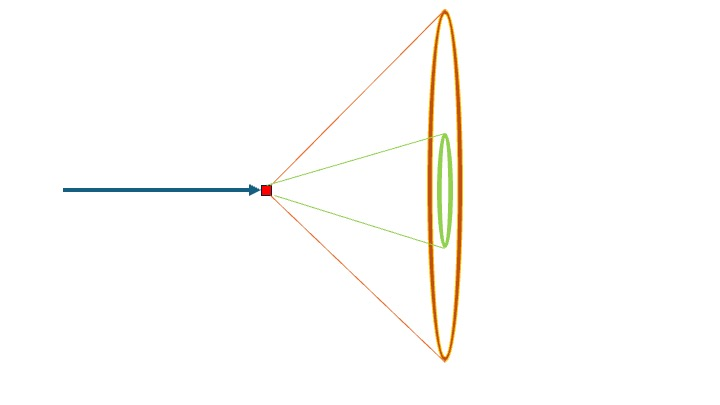
\includegraphics[width=0.9\linewidth]{figures/AxialDivergence1.jpeg}
        \caption{Side view}
    \end{subfigure}
    \begin{subfigure}{0.49\textwidth}
        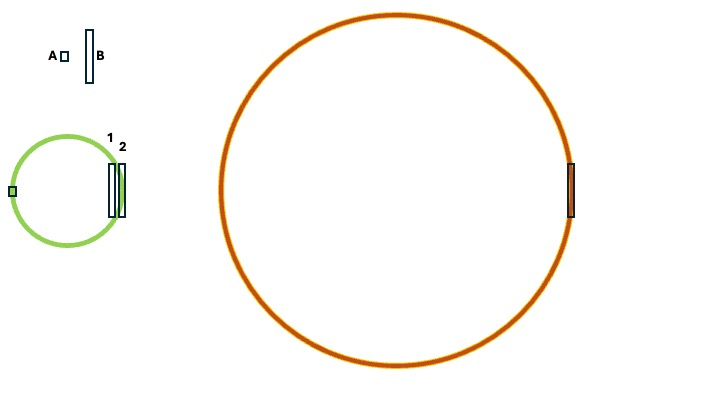
\includegraphics[width=0.9\linewidth]{figures/AxialDivergence2.jpeg}
        \caption{Viewed towards beam}
    \end{subfigure}
    
    \caption{Bragg diffraction cones for two reflections, one at low angle (green); one at higher angle (orange) viewed parallel to the diffracting beam (black arrow) and into the diffracting beam. The red square is the sample. Two slit sizes are shown. Note that the smaller slit (A) admits radiation to the detector from the low-angle cone only at the diffraction angle, but the elongated slit (B) admits radiation for the low-angle cone both at the proper angle (position 2) but also at lower angles, such as position 1. This effect is almost nonexistent for the higher angle Bragg cone.}
    \label{fig:cones}
\end{figure}

Likewise, in most instruments, the sample is also elongated in the direction of the $2\theta$ rotation circle. One can think of the effect of this as if there are a series of diffraction cones stacked along the elongation direction, as shown in Fig. \ref{fig:cones1}. This will cause the small slit to transmit radiation at angles lower than expected, thus causing approximately the same asymmetry as seen in Fig. \ref{fig:cones} with the elongated slit. Most commonly, the sample length and the slit length are matched. When both are elongated, the sample length accentuates the effect seen from the elongated slit. 

\begin{figure}
    \centering
    \begin{subfigure}{0.69\textwidth}
        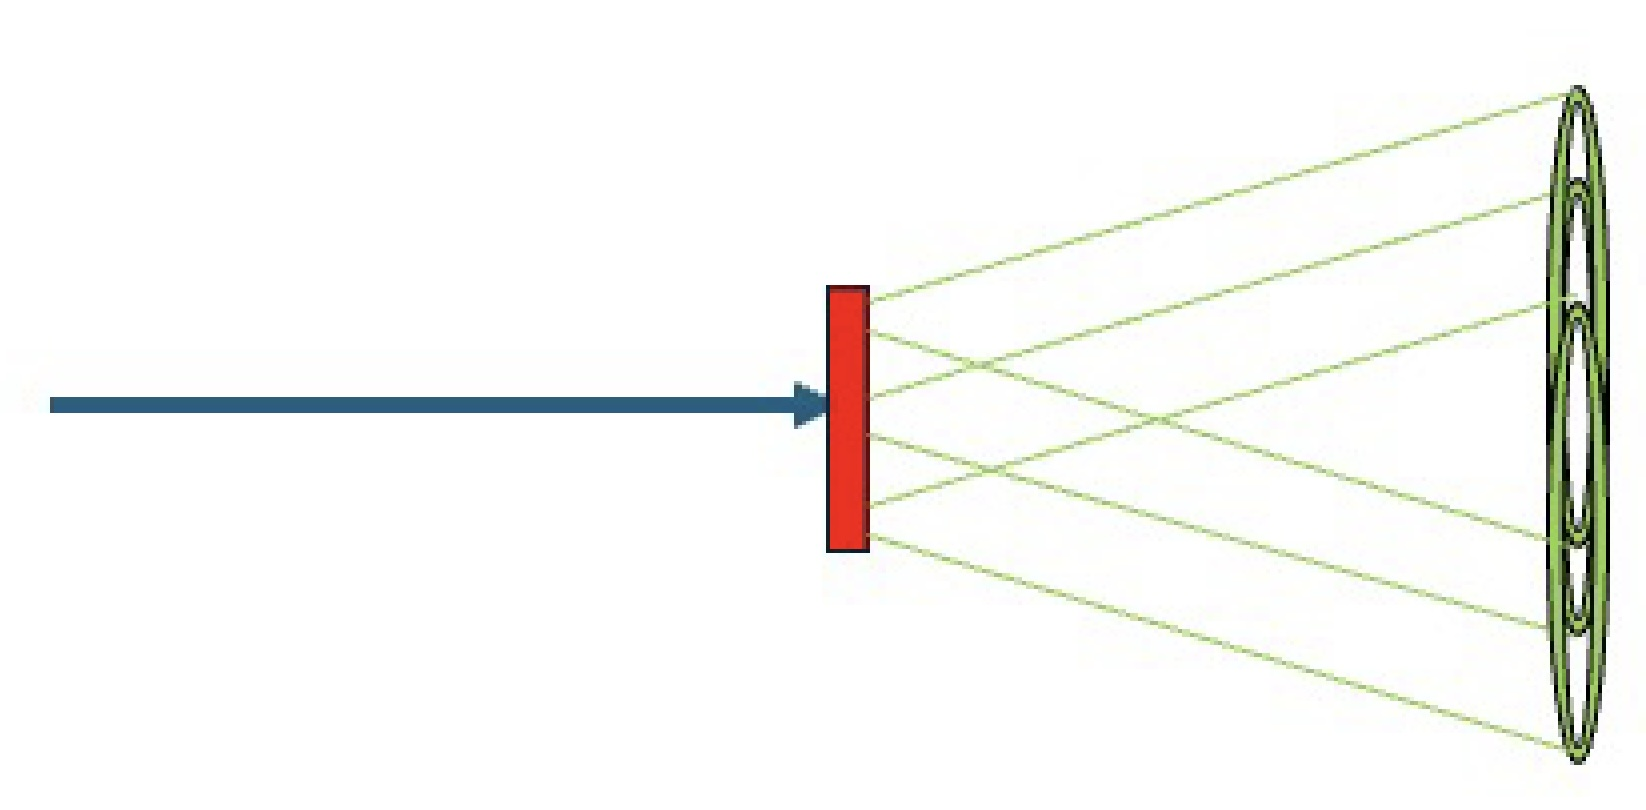
\includegraphics[width=0.9\linewidth]{figures/AxialDivergence3.jpeg}
        \caption{Side view}
    \end{subfigure}
        \begin{subfigure}{0.29\textwidth}
        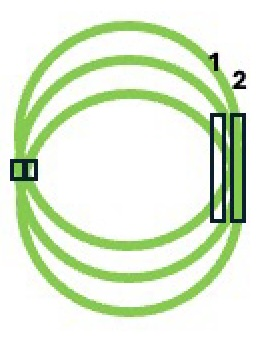
\includegraphics[width=0.9\linewidth]{figures/AxialDivergence4.jpeg}
        \caption{Viewed towards beam}
    \end{subfigure}
    \caption{Bragg diffraction cones from an elongated sample. Note that now a slit that is not elongated will see intensity at lowered $2\theta$ angles and an elongated slit sees additional intensity at low angles.}
    \label{fig:cones1}
\end{figure}

 Note that axial divergence does not occur with area detection. In such instruments the radiation source and sample sizes are minimized. The radial integration process does not cause this peak asymmetry. 

 

\section{Sample broadening}

Not only does the instrument create powder diffraction peak broadening, but all samples contribute broadening as well. While there are many types of defects in samples, such as stacking faults, screw dislocations or turbostratic disorder that can affect powder diffraction patterns, the two most significant effects are known as crystallite size broadening and microstrain broadening. Let us consider each effect. While instrumental broadening will depend only on the diffraction angle (or for TOF diffraction, both the angle and the wavelength), as we will see broadening can be different for different classes of reflections, where along some crystallographic directions, reflections will be broader than for other crystallographic directions. This is known as anisotropic peak broadening. While instrumental broadening is primarily Gaussian in nature, possibly with minor Lorentzian contributions, sample broadening is usually Lorentzian, though under unusual circumstances Gaussian contributions may be seen. 

 

\subsection{Crystallite size broadening}

As was noted in chapter \ref{Chap:diffraction}, diffraction arises from an infinite lattice of scatterers producing infinitely sharp diffraction maxima. Of course, all real crystals have finite size, so how does this affect diffraction? If we consider the diffraction from a single isolated crystal with a dimension \textit{d} (we will also consider the crystal to be spherical) then \textit{all} the diffraction maxima will be broadened in Q by a factor of 2$\pi$/\textit{d}, though the actual shape of the broadening function can be complex, particularly where \textit{d} is small, say with respect to 100*l. To relate this broadening to what is seen in measurements, we must consider that usually we measure diffraction patterns in experimental units such as an angle or for energy-dispersive measurements a unit (such as TOF) that we can relate to energy. Also, we have diffraction occurring from many crystalline domains, not one single crystalline particle, and further these domains may not be spherical. Let's consider each of these in turn.

While crystallite size causes the same broadening for all peaks \textit{measured in Q}, if we are looking at a plot of peak widths in degrees $2\theta$, we will see a change in peak widths. 
Noting that $Q = (4\pi/\lambda) \sin\theta$, the derivative dQ/d$\theta$ = ($4\pi/\lambda$) cos$\theta$. Inverting this, we see that if broadening of peaks is a constant amount $\Delta Q$, then $\Delta\theta = \Delta Q \lambda / [4\pi \cos\theta]$. Thus, crystallite size broadening, in units of $2\theta$, $\Delta 2\theta$ is proportional to $1/\cos\theta$. This broadening formulation was first developed a century ago by Paul Scherrer and is commonly written as 
$$\tau=\ {\frac{K\lambda}{\beta\cos{\theta}}}$$
where $\tau$ is the mean crystallite size in the same units as the wavelength (l); $\beta$ is the portion of full-width at half maximum of the peak that is due to crystallite broadening expressed in radians and $\theta$ is one half the $2\theta$ value for that peak. The unitless quantity K depends on the averaged morphology of the crystallites and is thus known as the shape factor. Winnie Wong-Ng in Volume H of the International Tables states that K will be in the approximate range of 0.6-2, depending on the assumption for this morphology, but is most commonly taken as 0.89. For GSAS-II we use K=1. 

\subsubsection{Anisotropic crystallite broadening}
 Note that crystallites need not have the same sizes in all directions. Anyone who has spent much time looking at powders, or for that matter minerals under a microscope knows that some materials will commonly grow with needle-like habits, where the size is much longer along one direction than in the perpendicular directions. Other materials, such as mica, may grow in a platy habit, where the length along one direction is much shorter than the perpendicular directions. With lower symmetry unit cells, many more complex unit cell anisotropic morphologies are possible. While crystallite broadening shows average properties for the entire sample that is illuminated, if the crystals have larger dimensions in some crystallographic directions than in others, we can expect to see broadening effects that differ for differing classes of reflections, since the class of the reflection (\textit{hk}0 reflections vs 00\textit{l}, for example) represent different orientations of the crystals. An easy analogy to think about the effect of orientation-dependent crystallite size on peak broadening is to imagine that the reflection “sees” the diffracting region in projection along the diffracting vector. Thus, if we consider the case where either needles or plates have their unique axis along the \textit{c} direction (this is a common case for hexagonal and tetragonal materials), we can see that the (00\textit{l}) reflections will have very different broadening from the (\textit{hk}0) reflections and the (\textit{hkl}) reflections will be intermediate between the two with the amount of broadening depending on the relative magnitudes of \textit{h}, \textit{k} and \textit{l}. In the case of needles, (00\textit{l}) reflections will be very sharp, since from that direction the crystal size is greatest. For plates, the (00\textit{l}) reflections will be very broad, since that will project as the smallest crystallite size direction. Thus, crystallite size broadening can be anisotropic when the average sizes of the crystal vary significantly by crystallographic direction. 

 Since powder diffraction is a phenomenon from a large number of crystallites and these crystallites will never all have exactly the same size, we must also consider that the distribution of crystallite sizes will convolute our size broadening. In theory it might be possible to back out the size distribution from the broadening effects and some papers have explored this, but I have not seen any convincing examples where this has been done. In powder diffraction we usually use scalar value(s) for crystallite size that represent some sort of mean value. 

 Note that I say crystallite size and not particle size here. While these terms are commonly interchanged in discussions, they mean quite different things. As an example, consider that most metal objects that we encounter are polycrystalline. (An example of an exception to that would be single-crystal titanium jet engine turbine blades.) My wedding band, for example, is a single discrete object and thus is a single particle, but it is likely composed of hundreds of thousands of crystallites. To define our terms, a crystallite is an ordered region of a material lacking long-range defects, though point defects may be present. The term grain is sometimes used for crystallite. In a somewhat circular definition, a crystallite can be considered as largest region that is seen as undisrupted ordered region by a diffraction probe, but it should be understood that different diffraction probes and even different reflections will see this differently. In contrast, a particle is a discrete object that could be a single crystal, a group of twined crystallites or even an agglomerate of randomly oriented crystallites or even could be multiphasic. Even what we call a single crystal is likely composed of multiple crystallites, since the preference for single-crystal diffraction measurements are “ideally imperfect” mosaic crystals made up of small crystalline domains that are in good, but not perfect alignment. Large non-mosaic single crystals are likely to exhibit extinction for intense reflections, which complicates structural analysis. 

 There are a number of different methods that are used for measuring particle size, which include light scattering, small angle x-ray or neutron scattering, physical separations, electrical sensing and imaging. These measure the sizes of agglomerate particles in a powder or liquid slurry. In contrast, diffraction, by x-rays, neutrons or even electrons, measures the size of the regions where atoms are scattering coherently, e.g. from a periodic lattice or even quasicrystalline domain. 

 Note that for some types of long-range faulting, some reflections may not be sensitive to the lapse in coherence caused by the fault, since in projection from a certain direction that fault might be invisible. Thus, in faulted materials some classes of reflections may be more broad than others. The faulted area might even appear to represent a longer-range structural motif in projection from certain directions and thus create new reflections that would be forbidden according to the long-range structure. This is why stacking faults can cause such complex changes in a powder diffraction pattern relative to an unfaulted material. The program DIFFaX from Treacy, Deem and Newsam, provides an excellent mechanism to model the effects of stacking faults on diffraction patterns, where a material is modeled as a set of layers where rather than having a fixed order of layering, as would be found in a fully crystalline material, probabilities are supplied for the likelihood for each type layer following the previous. GSAS-II incorporates the DIFFaX code and provides an interface for computation of faulted diffraction patterns. GSAS-II also provides visualization for the layers are joined to help prepare this relatively complex, but sometimes necessary, approach to describing a structural model. 

 When a characterization goal is to better understand the average crystallite shape or distribution of sizes, small-angle scattering is likely to be a better measurement than [wide-angle] powder diffraction. GSAS-II includes a program, Shapes, that is intended to model the mean particle size from small-angle scattering data. 

 

\subsection{Microstrain broadening}

The second type of sample broadening we will consider was historically called residual stress, but a better name for this is microstrain. To consider what this is about, let us imagine that we take a single crystal particle and put it into a C-clamp so that along one direction there is a force being applied to the crystal. For simplicity, let’s label that direction as the\textit{ c} axis. This force, which is called an external stress, will cause the \textit{c} axis to become slightly smaller since the lattice is being compressed by that force. If the same force were to be applied on the crystal uniformly, say by immersing the crystal into a container with a pressure-conducting liquid or gas and then squeezing on the container, we would then apply that force to all axes of our crystal. This would be hydrostatic stress. Thus, externally applied forces can change the lattice constants for a material. How much the lattice constants will change as a function of the force is described by a tensor populated by what are known as the elastic strain constants. The symmetry of the unit cell dictates the number of unique terms in this tensor, with 3 terms needed for a cubic system and 21 for triclinic. The name elastic stress implies that there can be a non-elastic condition. Elastic implies that if the force is released, the material will return to its original state. Indeed, if enough stress is applied, we can get outside the elastic regime. This will cause the crystal to undergo plastic deformation (think toothpaste) or catastrophic failure (cracking and breaking). 

 Now to get to back microstrain, imagine that I take a bunch of discrete unconnected crystals and put them into a container with random orientation and heat them to the point where crystals start to agglomerate, e.g. form connections to each other, but not hot enough so that the crystals start to recrystallize (where some crystals subsume others). When I remove the heat, I end up with a solid that has my crystals still randomly oriented as they started, but now the crystals are unable to move relative to each other since they are linked together. This heating process is known as sintering, but a similar process can occur when a molten material solidifies into a polycrystalline solid. Considering again our sintering material before we remove the heat, we can imagine that every crystal will have its lattice constants at equilibrium for that temperature. As the crystals start to cool, the lattice constants will get smaller, except the since there are now connections between the crystals, they are not free to shrink freely. If the contraction of the crystal lattices is at all anisotropic then some crystals will be trapped where they are unable to relax to their equilibrium lattice constants without breaking those connections. If they are unable to fully relax then they must be stretched (which we call being under strain). Since all forces must be matched, other crystals must be stress. This combination, which leads to an ensemble of crystals where there is a distribution of lattice constants, some larger than the equilibrium values and some smaller. This is the condition for residual stress. It commonly occurs in materials due to thermal and mechanical processing. 

 Microstrain broadening is really measuring the range of lattice constants in a material and there can other chemical effects that change the lattice constants for a microscopic section of a sample other than residual stress. A material may not have uniform chemical composition. The bonding of atoms close to a surface differs from that of atoms deep in the bulk (due to the truncated bonds at the surface or modified chemical environment for those atoms, should the surface be modified by oxygen or water, etc.) so the outer layers of particles may not have the same lattice constants as the bulk. 

 To consider the effect of microstrain on a powder diffraction pattern, consider the () diffraction from two crystals, one where the lattice parameter is at the equilibrium value for \textit{c}, but the other crystal has a slightly smaller lattice constant, \textit{c}-d. Recalling that $Q=2\pi d^\ast $ and for the 00\textit{l} reflections $d^\ast = l c^\ast$, we see that the reflection positions for 001, 002, 003,… reflections are, in units of Q, $2\pi c^\ast$, $2\pi c^\ast$, $2\pi c^\ast$,… If we consider the crystal that has a lattice constant of $c-\delta^\prime$, the reciprocal cell length will be $c^\ast+\delta$ and the reflection positions for those crystals will be $2\pi (c^\ast+\delta)$, $4\pi (c^\ast+\delta)$, $6\pi (c^\ast+\delta)$,… Thus, the difference in the peak positions will be $2\pi\delta$, $4\pi\delta$, $6\pi\delta$,… for Q values, $2\pi c^\ast$, $2\pi c^\ast$, $2\pi c^\ast$,… respectively. So, the spacing between the peaks from these two crystals increases as Q increases, meaning that the spacing between the peaks for each crystal is proportional to $\Delta Q/Q$. In a specimen with microstrain, we will have a distribution of lattice constants around the equilibrium value. This results in a distribution of peak positions which gives rise to peak broadening, but these peak positions also broaden proportional to $\Delta Q/Q$. 

 When looking at a diffraction pattern plotted in $2\theta$ units, we again must perform a coordinate transformation. Before we saw that $Q = (4\pi/\lambda) \sin\theta$ and $dQ = (4\pi/\lambda) \cos\theta d\theta$ so that $d\theta = (dQ/Q) (\sin\theta / \cos\theta)$ or equivalently $\Delta 2\theta$ is proportional to $\tan\theta$.

\subsubsection{Anisotropic microstrain broadening}

As noted, the range of lattice constants seen in a material can arise from multiple effects, including elastic strain. The elastic strain constants for a material can be highly anisotropic, which in other words means that a material will be much more “squishy” in some directions than others. As an example, if we consider graphite, which consists of hexagonal sheets of carbon atoms, the effect of applying pressure in the plane of the sheets would be expected to be quite different than applying pressure in the perpendicular direction to reduce the space between the sheets. Likewise, if a material has a range of compositions, the change in chemistry may well affect some lattice directions more than others. Either effect results in anisotropic microstrain broadening where some classes of reflections are affected more than others.


In conclusion, please understand that crystallite size broadening will be present in all powder diffraction samples, but it is often negligible since a diffraction instrument must have very good resolution to discern the broadening due to the size range for crystallites typically used for powder diffraction, e.g. microns; microstrain broadening will usually be present as well and it is typical for this to produce observable peak broadening. The one case where the reverse is commonly true, where crystallite size is observable and microstrain is not is in samples where very small crystallites have been created intentionally (nanoscale materials). With lower resolution instruments, it may not be possible to detect either type of broadening. Likewise, anisotropic peak broadening usually must be fairly significant to be detectable. 

The ability to differentiate crystallite size broadening from microstrain broadening depends on having discernible peaks over a sufficiently wide Q range. This is because the ability to distinguish the two sources of broadening depends on determining how that broadening changes with Q or $2\theta$. Noting that in Q, crystallite size broadens all peaks (for anisotropic broadening, in a hkl class) by the same amount, while microstrain broadening increases with Q, so that $\Delta Q/Q$ is constant. In $2\theta$ units, broadening will be proportional to $1/\cos\theta$ or $\tan\theta$, for crystallite size and microstrain, respectively. 

\section{Approaches for peak fitting functions}

Historically, there have been four different approaches used for computing powder diffraction peak profiles numerically to fit powder diffraction so that patterns may be fit. 

\begin{itemize}
\item
 One has been to use \textit{ad hoc} equations, such as the split Pearson VII function, which allows peak positions to be asymmetric because the low-Q and high-Q sides of the peak may differ in shape. 

\item
A second has been to use equations derived from physically-inspired (P-I) models. These equations are not an exact model for any instrument but are based on the underlying physics and offer adjustment factors to match performance. 

\item 
A third approach is one where a peak from the pattern is selected and then used to model the shape of all peaks in the pattern. This was developed by Christian Baerlocher\index{Baerlocher, C.} and co-workers and has been called a “learned” peak shape. It is not commonly used.

\item 
The newest method for modeling peak shapes is called the fundamental parameters approach (FPA). In this, the broadening effect from each optical component in an instrument is defined and the instrumental peak shape is determined by convoluting each of these terms, along with terms for the sample broadening. Commonly some adjustment factors are also used. 
\end{itemize}

 The \textit{ad hoc} approach for fitting is less than ideal because it can allow inclusion of effects that are not physically possible. As an example for why this is the case, the asymmetric peak broadening in low angle diffraction peaks due to axial divergence not only causes the peak to have the low-Q and high-Q sides of peaks to have different widths, but it shifts the peak positions as well. Since these shifts will not be accounted for in the \textit{ad hoc} equations, the fitting software will not compute the lattice parameters optimally. Use of learned peak shapes can handle aberrations that introduce irregular aspects to the peak shape, but it fails to handle anisotropic or Q dependent broaden effects. The greater use of machine learning techniques in recent years may mean that this approach may yet see a future renaissance. The physically-inspired approach was used in Hugo Rietveld’s initial codes and has been augmented over the decades as the basic physics description has improved. It is available in all of widely used Rietveld codes. Despite this, the FPA method has several nice features. Only a small number of codes implement FPA-generated peak shapes, but those codes are seeing wide use. If an instrument is well described, then no fitting parameters are needed to model a pattern’s peak profiles, other than for sample-related effects. The FPA method has the potential to reproduce minor deviations of the profile from the shapes produced from even the most advanced P-I functions. Creating the FPA model for a novel instrument is not a simple task, even for an FPA expert, but once done FPA fitting is unmatched for proving that an instrument is performing at the level expected for how it was designed. 

 However, my personal opinion is that the improvements in peak shape fitting from FPA for modern commercial instruments are of negligible value to improve the accuracy for the parameters derived from Rietveld analysis. For this reason, our choice in GSAS-II has been to use a physically-inspired peak shape model. It fits the profiles from laboratory instruments, as well as very specialized synchrotron and neutron instruments, well enough that the sample can be very accurately modeled and characterized; this is the goal for Rietveld analysis.

 The one valid criticism of the GSAS-II model is that fundamental parameters profile computations have the ability to describe \textit{instrumental} peak shape functions that are not well-fit by the pseudo-Voigt function that GSAS-II uses. However, modern diffraction instruments rarely have significant deviations from a pseudo-Voigt function peak shape and even where that can be noted, the contribution of the slight misfit to the model fitting results will be negligible. However, in theory with FPA one could develop sample broadening models that account for more complex treatment of sample broadening (for example, a bimodal crystallite size distribution or where defects create asymmetric broadening), but as far as I am aware no one has developed a generalized methodology for this with FPA. 

 

\section{Physically-Inspired Peak Shapes}

The forerunner to modern P-I functions was work by Caglioti\index{Caglioti, G.} et al. in 1958 (the year of my birth!) where he and co-workers characterized the instrumental resolution expected from mosaic neutron monochromators and found that broadening should be Gaussian and follow a curve where the resolution minimum is close to the monochromator takeoff angle. From this Hugo Rietveld\index{Rietveld, H.} developed a resolution curve where the Gaussian broadening function is written as $\sigma^2\ =\ U\ \tan^2{\theta}\ +V\ \tan{\theta}+W$, and this expression is now known as the Caglioti equation. In this equation, $\sigma=FWHM\ /\ \sqrt{8\ln{2}}$ ($FWHM$ is the full-width at half maximum) and $U$, $V$ and $W$ are terms determined for the instrumental configuration. This equation was not developed for x-rays, but in truth Caglioti equation is simply a polynomial and has the flexibility to fit instruments of all types. Ted Prince\index{Prince, E.} pointed out that the fitting process is much more stable if the equation is reformulated as $\sigma^2\ =\ U^\prime\ \tan^2{\left(\theta-\theta_m\right)}\ +V^\prime\ \tan{(\theta}-\theta_m)+W^\prime$, where $\theta_m $ is the monochromator “takeoff” angle. Ted was completely correct on this, but no one other than he ever implemented the modified equation in a Rietveld code. Whenever you find fitting the $U$, $V$ \& $W$ terms to be difficult, I invite you to curse the code developers (alas, I am on that list) who did not listen to Ted. 

When Rietveld analysis was initially adapted to treat x-ray data, it became clear that the pure-Gaussian peak shape initially used was inadequate for treatment of x-ray line shapes. This is because the peaks had the longer tails seen in a Lorentzian function (this is also sometimes called a Cauchy function). This is mostly because the better resolution of x-ray instruments at low angles in comparison to the neutron instruments at that time was better able to show sample broadening effects, which are largely Lorentzian. After considerable discussion in the literature, the Voigt function, which is a convolution of a Gaussian and Lorentzian function, was accepted as a good descriptor for powder diffraction peak shapes. The Voigt function is relatively slow to compute, so a substitute for this is commonly used, where a Gaussian and Lorentzian function are multiplied rather than convoluted. This produces a peak shape that is quite close to that from a similarly parameterized Voigt function. The powder diffraction community calls this product a pseudo-Voigt and it is a good approximation for the Voigt. One of my early activities in Rietveld analysis was to take a Rietveld code that used a pseudo-Voigt peak shape and add an option to instead compute a Voigt peak shape function instead. The result was a refinement that was considerably slower than the original where improvement in the fit was nearly imperceptible. My option was never used after that. 

 The commonly used form for the Lorentzian contribution to the profile is $FWHM\ =\ X\ /\ \cos{\theta}\ +Y\ \tan{\theta}$. Note that X and Y are the broadening contributions expected from crystallite size and microstrain broadening, respectively, and thus might not be the best choices for describing instrumental broadening, but these two terms together provide quite a bit of flexibility in fitting the broadening, particularly considering that Lorentzian contributions to instrumental broadening tend to be minor. As will be discussed further, below, GSAS-II introduces a third term to offer even more flexibility in the treatment of CW broadening, but it is not clear that this is ever needed. 

 One other significant improvement seen in peak shape functions was treatment for the asymmetry seen in low angle peaks due to axial divergence. The history here is that Hugo Rietveld\index{Rietveld, H.} introduced an \textit{ad hoc} correction for low angle asymmetry that did not work very well. Several other unsatisfactory treatments were tried later. The physical cause of this low angle asymmetry was well understood quite early (and is well explained in Klug \& Alexander’s 1974 book) but was first formulated in integral form in 1984 by Van Laar and Yelon, but that formalism was not conducive for peak shape computation. In 1986 Eddy\index{Eddy, M.}, Cheetham\index{Cheetham, A.} and David\index{David, W. I. F.} published a paper demonstrating that low-angle asymmetry could be fit well using the Van Laar and Yelon approach, but did not make their code available. In 1994, Finger, Cox\index{Cox, D.} and Jephcoat\index{Jephcoat, A.}, who were not then aware of the Eddy et al work, revisited the Van Laar and Yelon work, correcting some of the math. Larry Finger\index{Finger, L.}, who was a friend and prized role model to me, not only published this work, but also distributed their peak shape computation code and encouraged its employment in other software. The result is that this work is now known as the Finger-Cox-Jephcoat (FCJ) correction. While this does short-change the contribution from my very much respected friends Mike Eddy, Tony Cheetham and Bill David, I do use this naming as well; there is a moral somewhere in this about the value of putting one’s ideas into tools that others can use.

 The FCJ correction requires three parameters, the diffractometer radius (L), the length of the sample (S) and the length of the detector slit (H), where these lengths are measured along the diffractometer axis of rotation (perpendicular to the diffraction plane). The radius is used as a ratio with each of the lengths so there are really only two free parameters. These parameters in theory are known and should not need to be fit, but indeed must be adjusted when x-ray or neutron focusing is used. The two lengths have very similar effects on asymmetry and thus usually cannot be refined together. 

 These three contributions, the $U$, $V$, $W$ parameterized Gaussian function, the $X$ and $Y$ parameterized Lorentzian function, and the FCJ correction, form the backbone for P-I descriptions of peak shapes for constant-wavelength neutron and x-ray instruments in most Rietveld software, though some additional terms may be incorporated. 

 Things are quite different for TOF neutrons, which require a much more complex formulation to account for the performance of the neutron moderator, the neutron guides and path length of the instrument and the arrangement of detectors. Many different approaches have been used. The specific model used in GSAS-II was developed by my partner in GSAS-II development, Bob Von Dreele\index{Von Dreele, R. B.}, based on his unique expertise in TOF instrumentation that goes back to the initial development of the technique. Note that the parameters used to fit the instrumental broadening for a TOF instrument are determined by the facility and instrument design, which is largely fixed, though perturbations may be offered through changes in collimation options and frame selection via chopper settings. Fitting the TOF profile terms can be a tricky process, since more than one combination of values can produce comparable fits. This fitting is best done periodically by an instrument scientist, who will supply profile values along with reduced data suitable for input to a refinement. 

 

\section{GSAS-II Profile Implementation}

The creation of GSAS-II provided us with the option to rethink how profiles are handled in Rietveld. In earlier programs, such as GSAS/EXPGUI, a single set of profile terms are provided to describe both the instrumental and sample broadening effects. Even when broadening for an instrument was well-characterized, as is common for user instruments at neutron sources, the mixing of instrumental and sample contributions in the refinement stage made it difficult to discern which was which. 

 This was not a serious problem with the initial role for Rietveld fitting, where a diffraction dataset was collected (perhaps with less care than desirable for the reproducibility in the instrumental settings,) from a material that consisted primarily of a single phase and where the goal was a crystal structure determination for that primary phase. Fitting of broadening was a necessary chore, and learning the profile parameters was not typically a goal. We now use Rietveld for so many more types of measurements. When considering a more common contemporary use-case for Rietveld, we are likely to have data from a well-characterized diffractometer on a multiphase material. Rietveld is commonly employed for materials where the atomic structures are well understood, but we want to learn about materials effects, such as microstrain or phase composition or details for site substitutions or lattice constants or perhaps how the material evolves with time or the application of temperature, an external electric field, pressure, etc. From this perspective we realize that the instrumental contributions for broadening should be the same for all datasets from that instrumental configuration. Further, in the ideal case those effects will be known and will not require fitting. On the other hand, crystallite size and microstrain will not be known in advance, will be different for every phase and may change over the course of a parametric experiment. Further, more complex models for anisotropic sample broadening may be needed for some phases, but not others. From this perspective it becomes clear that one wants the ability to separate instrumental and sample broadening contributions. 

 For this reason, GSAS-II associates instrumental broadening terms with each PWDR (powder) histogram, where the initial values for the parameters are read from the instrument parameter file used when the dataset histogram is initially imported. The sample broadening terms are considered both a property of the phase (as there is no reason that two different phases would be expected to have the same crystallite sizes or microstrain) but also a property of the histogram, since the specimen used for each measurement might have differing sizes or morphologies. Thus, there are independent values for sample broadening for every histogram in every phase, so if there are $m$ histograms and $n$ phases, there will be $n \times m$ sets of sample broadening terms. Bob and I call such parameters HAP parameters (histogram-and-phase) in a name that dates back to the original GSAS program. Note that where one wishes to force sample broadening values to be the same, for example where the same specimen is used in multiple histograms, constraints can be used to group the values. These HAP parameters are placed in a location of the GSAS-II data structure associated with each phase, but there is some choice on how they appear in the GUI. This will be discussed further below.

 

\subsection{GSAS-II Instrumental Profile Treatment}

GSAS-II places the instrumental broadening terms into the “Instrument Parameters” section of each PWDR (powder) histogram. The instrumental parameters for sample broadening for CW x-ray and neutron histograms consist of U, V, and W, as described as above. For TOF neutron histograms, the peak shape is generated from convolution of double exponential and pseudo-Voigt. The exponential parameters are split between the “rise side” (shorter TOF, or equivalently high Q) and the “decay side” (longer TOF or small Q). On the low TOF side of the peak, there is one parameter a, which is multiplied by d*. One the high TOF side of the peak, there are three terms, b\textsubscript{0}, b\textsubscript{1} and b\textsubscript{q}, which are scaled by 1, d*\textsuperscript{2} and d*\textsuperscript{4}, respectively. The pseudo-Voigt is parameterized where the variance for the Gaussian contribution to the peak, $\sigma$, ($\sigma=FWHM\ /\ \sqrt{8\ln{2}}$) is determined from 
$$\sigma\ =\ \sigma_0\ +\ \frac{\sigma_1}{d^{\ast2}}\ +\ \frac{\sigma_2}{d^{\ast4}}\ +\ \frac{\sigma_q}{d^\ast}$$
and the Lorentzian contribution, g, (g = FWHM) is determined from
$$\gamma=\frac{X}{d^\ast}+\frac{Y}{d^{\ast2}}+Z$$
There are theoretical reasons for the choice of these functions, but the parameterization is largely determined from experience with a variety of TOF instruments. Most instruments do not require all these terms for a good fit, but each of these terms has been needed for a good fit for at least one instrument. 

In GSAS-II, the three terms used in the FCJ correction for low-angle peak asymmetry (S, H, \& L) are reduced to a single value (S+H)/L with S=H and this parameter is much more stable with respect to refinement.

 
\section{GSAS-II Sample Broadening Terms}
\index{HAP parameters|textbf}\label{ref:HAP}

GSAS-II offers separate terms for crystallite broadening and for microstrain and those terms can be applied isotropically or two models are provided for anisotropic broadening for each. As was noted before, there are sample broadening terms associated with each histogram for each phase, so if there are $m$ histograms and $n$ phases, there will be $m \times n$ sets of sample broadening terms. 

\subsection{GSAS-II Size Broadening Models}

For crystallite broadening, the GSAS-II offers three models, which will be discussed directly below. 

\subsubsection{Isotropic}
 The default broadening model is labeled as isotropic, which of course assumes a uniform crystallite size in all directions. This model has two refinable parameters: One is for the mean crystallite size and the second, labeled LGmix, determines if the broadening will be Lorentzian, Gaussian or a mix between the two.

 The isotropic crystallite size parameter has units of mm (10\textsuperscript{-6} m). This is determined using the Scherrer equation with a K value of unity. While K=1 does not exactly match the most common crystallite morphologies that are encountered, we consider that crystallite broadening is not a rigorously defined quantity, so while relative differences between measurements on different specimens of the same sample may be determined quite accurately, no one should ever be concerned about a discrepancy of 10\% between different quantification methods or as a difference from measurements on different materials, where the morphology may differ. Note that as the crystallite size parameter decreases, more broadening occurs, while larger values provide very minimal broadening. From a practical perspective, the instrumental resolution limits the maximum value of crystallite size broadening that can be discerned from a dataset. 
 GSAS-II does not allow the crystallite size to refine below 0.01 $\mu$m. At this value peaks are so broad as to defeat Rietveld analysis. It the size parameter also is not allowed to refine above 10 $\mu$m, which would produce imperceptible broadening with any existing powder diffractometer. In practice, with a very high resolution instrument, values above perhaps 3 $\mu$m are meaningless. More typical for most diffractometers may be 1 $\mu$m. It is the user’s responsibility to review the refined value for the size parameter and to eliminate refinement for this parameter once the value is above the discernible range for the instrument that has been used.

 The default for LGmix is 1, which means the peaks will be 100\% Lorentzian. If LGmix is 0 then the crystallite broadening would be 100\% Gaussian and values between 0 and 1 create a linear mix between the two. Physically, an LGmix value of 1 is what is expected, except from materials that have a very unusual distribution of crystallite sizes, such as a monodisperse size. While the parameter LGmix can be varied, values other than 1 seldom improves a fit. Unless a significant improvement is seen for other values, the value is best fixed at 1. Values less than 0 or greater than 1 represent peak shape functions that are highly unlikely, but I am not comfortable saying that they are always physically impossible. Seeing a value other than unity most likely indicates a problem with the background fitting, but perhaps could arise from something very unusual in crystallite size distributions. I will only change LGmix from unity if I have extreme problems in obtaining a good fit to the peak profile. 

 \subsubsection{Uniaxial}
 When there is evidence for anisotropic peak broadening and the broadening arises primarily from crystallite size, a more advanced model is that of uniaxial size broadening. This describes the average crystallite shape as a cylindrical, which in extreme cases extends to platy or needlelike morphologies. For this, one provides the crystallographic direction for the axis of the cylinder and this model provides two size parameters, axial and equatorial sizes, which again have $\mu$m units and are otherwise similar to the previous isotropic value except that the axial value is the average size value along the specified crystallographic direction and the equatorial value is the size perpendicular to that direction. There is also a single LGmix parameter to describe the Lorentzian vs. Gaussian character of the broadening, which again is rarely any value other than one. 

 Picking axes to select for broadening can be a trial-and-error process. For some Bravais lattice choices, there is only one sensible axis for broadening: For tetragonal, hexagonal or rhombohedral (hexagonal setting) the (001) axis is unique. [Note that for rhombohedral space groups in a rhombohedric setting, the (111) axis is equivalent to the hexagonal (001) axis and thus is unique.] For cubic cells, there are effectively three unique and non-perpendicular axes (001), (110) and (111). Highly anisotropic habits in cubic systems are unusual but uniaxial broadening nonetheless can be attempted to see if the fit improves. For orthorhombic, monoclinic and triclinic cells, there are no symmetry-based restrictions on preferred broadening directions, but analysis of peak widths may suggest a direction that has the broadest or narrowest widths or trial-and-error may suggest a preferred axis that improves the fit significantly. 

 \subsubsection{Ellipsoidal}
 The remaining crystallite size broadening model that GSAS-II offers is labeled ellipsoidal, as the average crystallite is assumed to have a shape described by a tensor that is analogous to the anisotropic displacement parameter (ADP) ellipsoid. The terms in the tensor are labeled by GSAS-II as S\textit{ij}. The diagonal elements (\textit{i}=\textit{j}) of the tensor specify crystallite lengths along three orthogonal axes and the off-diagonal terms (\textit{i}¹\textit{j}) orient the ellipsoid relative to the cell axes. Thus, there are six terms to refine, though one may want to start with only the diagonal terms. Note that in higher symmetry Bravais lattices, just as for ADP’s for atoms on high-symmetry sites, symmetry may require constraints, but at present GSAS-II does not force this. Thus, use of this model is not recommended for cubic, hexagonal/rhombohedral or tetragonal symmetry, unless users understand the symmetry implications on the tensor terms.

 

\subsection{GSAS-II Microstrain Broadening Models}

\subsubsection{Isotropic}
For microstrain broadening, the GSAS-II default broadening model is also labeled as isotropic, and again assumes microstrain is uniform in all directions. As is the case for isotropic crystallite size broadening, this model has two parameters: One is for the mean microstrain and the second, labeled LGmix, determines if the broadening will be Lorentzian, Gaussian or a mix between the two. 

 The microstrain parameter is the unitless quantity $\Delta Q/Q \times 10^6$. Note that this value has the opposite broadening effect from the crystallite size parameter. Smaller values produce less broadening. The default of value for microstrain is 1000, which can be considered a lower limit value for most diffractometers. (With 11-BM and other high-resolution diffractometers, one can see broadening with microstrain in the range of 300-500, perhaps). If the value decreases to a value that is insignificant, reset it and turn off the refinement of this parameter.

 The default again for LGmix is 1, which means the peaks will be 100\% Lorentzian. This parameter can be varied, but it seldom improves fits and unless a significant improvement is seen for other values, the value is best fixed at 1. I am unable to imagine what could give rise to an LGmix values less than 0 or greater than 1, but perhaps there might be physical reasons why this might be the case. Again, if I see a significant improvement in a fit when LGmix refines to a value outside the range of 0-1, I would look carefully to make sure the background fit is reasonable.

 \subsubsection{Uniaxial}
 When there is evidence for anisotropic peak microstrain broadening, the next model to try is that of uniaxial microstrain broadening, which is very much analogous to the uniaxial crystallite size broadening model. Here, this describes a system where the material is either much more stiff or much softer in one direction, particularly compared to the perpendicular directions. Again, one provides the crystallographic direction for this unique direction and again there are now two microstrain parameters, axial and equatorial, which again are $\Delta Q/Q \times 10^6$ (unitless). There is a single LGmix parameter to describe the Lorentzian vs. Gaussian character of the broadening, which again is rarely any value less than one. The same discussion for selecting a broadening axes from uniaxial crystallite size broadening applies here as well. 

 \subsubsection{Generalized}
 The third model for microstrain is labeled as “generalized” and is based on the work of Popa and Stephens to expand microstrain with symmetry-consistent Bessel function terms. The number of terms provided depends on the Laue class for the phase, but because these terms must be consistent with lattice symmetry, they usually refine with good stability. Unlike the elliptical case for crystallite size broadening, one can try fitting with the generalized microstrain model in a routine manner. 

 

\section{GUI Access to Sample Broadening Terms}

 As noted, sample broadening is treated in GSAS-II as both a property of the phase (as there is no reason that two different phases would be expected to have the same crystallite sizes or microstrain) but also a property of the histogram (since the specimen used for each measurement might have differing sizes or morphologies.) One can define constraints that force the size parameters to be the same across datasets (which might be useful where the same batch of material was used for all measurements). I have used this for impurity phases, where too few peaks to fit broadening well for all phases. By default, these “HAP” parameters are found on each Phase’s Data tab, as seen in Fig. \ref{fig:size1} where I have outlined the crystallite size values in yellow.

\begin{figure}
    \centering
    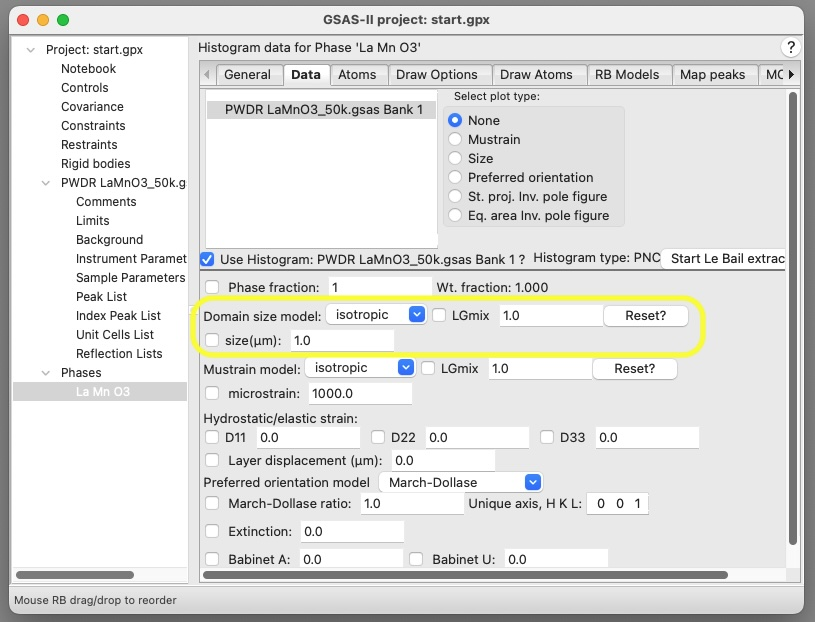
\includegraphics[width=0.75\linewidth]{figures/size1.jpg}
    \caption{Location of crystallite size parameters in the default data tab of the Phase.}
    \label{fig:size1}
\end{figure}

The phase is selected from the data tree and the histogram is selected from box to the upper left. Menu commands allow duplication of the parameter values between different histograms. Copying of values can be done where all values are copied (menu command “Copy data”) or where only selected values are copied (menu command “Copy selected data”). It is also possible to duplicate only the refinement settings (we call them refinement flags) with the “Copy flags” menu command. There is no mechanism at present for copying values between phases. 

\subsection{Placing HAP parameters directly into data tree}\label{ref:separatehistogram}

 Note that GSAS-II offers a mode where these “HAP” values are placed in their own data tree entry. (I prefer this mode.) This mode is selected using the preference variable “SeparateHistPhaseTreeItem” as shown in Fig. \ref{fig:HAPmode}. 

\begin{figure}
    \centering
    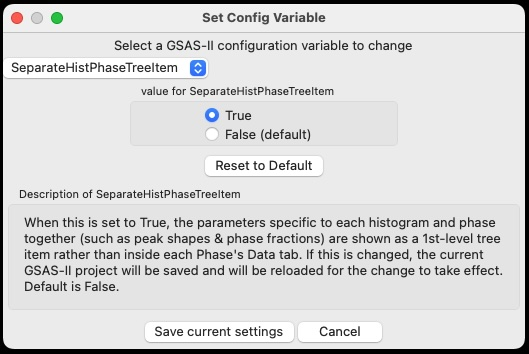
\includegraphics[width=0.5\linewidth]{figures/SeparateHAP.jpg}
    \caption{Figure 4: Setting to put the HAP entries in a separate tree entry}
    \label{fig:HAPmode}
\end{figure}

When this is done, these entries are accessed in the Hist/Phase item in the data tree and the window has a slightly different appearance (note that phases are now selected using the tabs at the top of the window), as seen in Fig. \ref{fig:size2}.

\begin{figure}
    \centering
    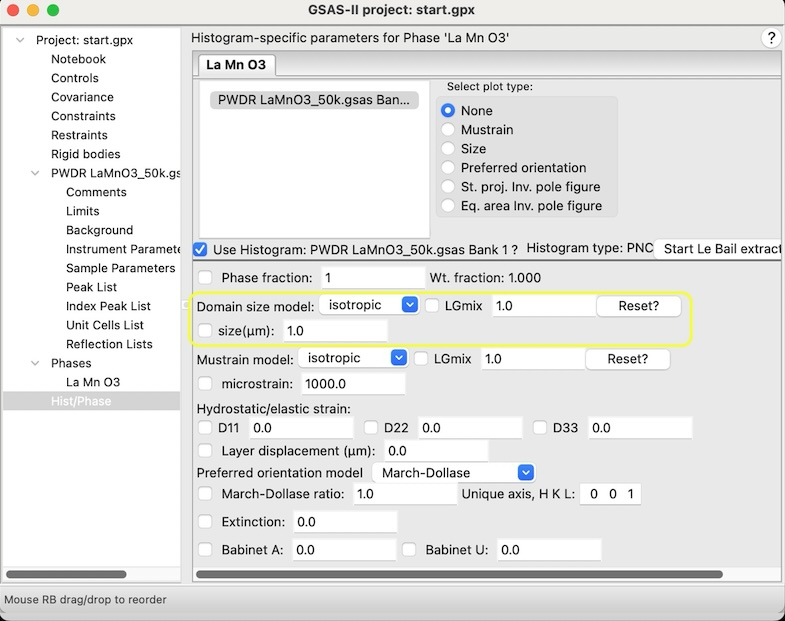
\includegraphics[width=0.75\linewidth]{figures/size2.jpg}\caption{Size parameter location with optional setting to place the HAP settings in a separate data tree entry}
    \label{fig:size2}
\end{figure}

 

\section{GSAS-II Sample Broadening Visualization}

While the isotropic crystallite size and microstrain terms have no geometric implications, interpreting the anisotropic models from the numerical values is a challenge, particularly for the third form of each set. For this reason GSAS-II allows one to visualize the model for the average for the crystallite size and microstrain values in 3-D as a function of geometry. This is done in the GUI by selecting the plot type in the upper right as “Size” for crystallite size and “Mustrain” for microstrain. For the isotropic models a sphere is plotted, but for the uniaxial case it may be of some value to visualize the relative sizes of the on-axis vs. perpendicular broadening. For the ellipsoidal case, this is more useful as it shows both the lengths and orientation of the crystallite model. The plots for microstrain fitting from the generalized Stephens/Popa model can be unusual shapes where there is considerably more microstrain in directions diagonal to crystal axes, as opposed to along the crystal axes. Since overfitting, where too many terms are introduced, is a constant concern in Rietveld analysis, it is always worthwhile to look at this plot and consider if the values make sense with what is known about the material. 

 

\section{Determining Instrumental Profile Terms}\label{ref:DeterminingInstrumental}

The preferred way that GSAS-II will be used will have these instrumental broadening terms determined for the instrumental configuration before a dataset is imported. Ideally, someone else will have carefully determined these values for you (for example at a synchrotron or neutron source, or in a well-run x-ray lab). If those values are provided to you as an .instprm file (or in the format used by the original GSAS code, where .INS, .prm and .inst are common extensions), you can read these values in with your dataset and then ignore them while you work on fitting aspect of your sample that you care about. This greatly simplifies the process of fitting diffraction data. This is especially true with TOF data where the instrumental profile terms are quite complex. 

Note that if your instrument has configuration options, such as changeable collimation (slits), a moveable detector or neutron chopper settings, these will affect the instrument resolution and the instrumental broadening terms need to match the configuration used for data collection. 

 If you do not have these instrumental broadening terms for your instrument, you are best off collecting a diffraction pattern with a standard to calibrate the instrument. You want to collect data over the same range that you will use for data collection on samples, or perhaps a wider range. The standard should have sharp peaks over a wide angular range and ideally should have known crystallite sizes and microstrain. The NIST Standard Reference Material 660 (LaB\textsubscript{6}) is an excellent choice for this, particularly the 660c version, which is made with \textsuperscript{11}B, so that it can be used for neutrons as well as x-rays, but is expensive -- if it can even be located for purchase. Some samples of Na\textsubscript{2}Al\textsubscript{2}Ca\textsubscript{3}F\textsubscript{14} (commonly called NAC) have been produced that have even sharper peaks than NIST LaB\textsubscript{6}. Silver behenate [CH\textsubscript{3}(CH\textsubscript{2})\textsubscript{20}COOAg] is commonly used for sharp lines at low diffraction angles. Many inexpensive materials can be obtained that produce sharp diffraction peaks with minimal microstrain and crystallite broadening, but often these materials have small unit cells and do not diffract at low angles. However, scans of multiple materials to provide diffraction peaks at low as well as high angles or even a mixture could provide an inexpensive secondary standard for diffraction line profiles. Work on this would be very useful to the community. Measurement and fitting of data on standard(s) for an uncharacterized instrument has the additional advantage that it demonstrates that the instrument is performing well. If a standard cannot be well-fit, then it is quite unlikely that more complex studies can be completed with better results, as there is an instrument alignment or problematic performance issue (such as x-ray tube contamination). 

 After collecting data on a standard, one should read the data into GSAS-II. The GUI will then ask you to provide an instrument parameter file, but if you do not have one with reasonable parameters, you can press “Cancel” on that dialog and a second window will offer choices with default options. 

 Fitting profile terms to data for a standard can be a surprisingly difficult task when starting from values well away from an optimal set. GSAS-II provides two tutorials\footnote{GSAS-II tutorials can be viewed using the Help/Tutorials menu command or at web page \url{https://advancedphotonsource.github.io/GSAS-II-tutorials/tutorials.html}}  
 ``Create Instrument Parameter File: Determine Starting Profile from a Standard”
 for a laboratory instrument and 
 ``Calibration of a Neutron TOF diffractometer” that run through the process of this fitting. Note that optimal profile term fitting requires that the background, lattice constants and peak intensities all be well fit, in addition to the peak profiles. If, for example, the background is too low in the region of some peaks, then profile fitting will tend to widen peaks and artificially increase the Lorentzian contribution to the peak(s) so that the peak tails contribute to what should be modeled as background scattering. 

 Note that instrumental broadening is typically Gaussian and sample broadening Lorentzian, so when fitting the instrumental terms, the X \& Y terms should initially be set to zero and only U, V \& W be refined for CW instruments. Non-zero values for X \& Y are rare and if refined, this should be where the crystallite size and microstrain values are set to known values. One should never refine X \& Y and either the crystallite size or microstrain together. 

 

\section{FPA Generation of Instrumental Terms}

If the diffraction instrument’s optical properties are well characterized, then it is possible to construct a description of the expected peak profiles using the fundamental parameters approach (FPA). While FPA models have been developed for synchrotron and neutron diffractometers, this is primarily the domain of laboratory x-ray diffractometers. GSAS-II provides a module where FPA terms may be input and an automatic process then 

generates peak profiles as a function of $2\theta$ and fits them with the GSAS-II profile coefficients. These profile terms are then used to generate an instrument parameter file. The FPA profiles are generated with the NIST ``Fundamental Parameters Python Code'' from Marcus H. Mendenhall et al. that is included in GSAS-II. To access this capability, use the “Fit instr. profile from fundamental parms” command in the Powder Diffraction submenu in the Imports menu; also see the ``Determining Profile Parameters with Fundamental Parameters'' tutorial. 


\section{How to Refine Peak Profiles for a Sample}

There are three usual cases for how peak profiles might be fit with GSAS-II: 

\begin{enumerate}
\item The preferred case, where the instrument is well characterized and only sample terms need to be refined. 

\item Where one must work with a dataset without known instrumental broadening terms. 

\item Where an instrument is being characterized to determine the instrumental broadening terms. 
\end{enumerate}

The third case has been discussed previously in the “Determining Instrumental Profile Terms” section, \S\ref{ref:DeterminingInstrumental}. The second case is to be avoided wherever possible, but will be discussed further, below. So, I will first consider the process for fitting the sample broadening terms when the instrumental terms have already been determined for the instrument configuration used for data collection, which is what I would prefer to see people do. Good fits for peak profiles are only possible when the peak locations (from lattice parameters and sample displacement parameters), background and reflection intensities are all well fit. Thus, there are four interlocking aspects of Rietveld fitting. Please be sure to read the chapters on peak position (Chapter \ref{Chap:peakpositions}), background (Chapter \ref{Chap:background}), and peak intensity fitting (Chapter \ref{Chap:intensities}) before attempting to fit sample broadening.

\subsection{Refinement of sample terms only}

The optimal way that GSAS-II profiles will be fit will be to use previously determined profile terms that accurately describe the instrumental contribution to peak profiles. When this is the case then a good fit for the observed peak profiles should be obtained with refinement of the sample terms and the instrumental broadening terms do not need to be fit for samples. This greatly simplifies the Rietveld fitting process. In very simple cases, it will be possible to refine the histogram scale factor, background, lattice parameters and sample broadening all at the same time, but when any of those parameters start fairly far from their optimum values, the refinement may move to unreasonable values for some parameters and once that happens further optimization may not be possible. For this reason, I recommend a more systematic approach where parameters are added to the model in a more deliberate sequence. 

 Note that for complex crystallographic studies, where the starting model will not fit the diffraction intensities well (since improving an inaccurate model is the point of the study), it will not be possible to fit peak profiles well with the starting model; but it may also be impossible to fit the crystallographic structure with a poorly-fit peak shape. One approach to this is to cycle between fitting the background, then the peak shape, then the structure, (while also optimizing the unit cell parameters) and keep returning to each of these and possibly adding new parameters, such as sample displacement and preferred orientation, in turn until an optimum fit has been obtained. To remove intensity fitting from the combined tasks for fitting all aspects of the data, some researchers perform an initial profile fitting using a Le Bail\index{Le Bail fitting} or Pawley\index{Pawley fitting} fit (see \S\ref{ref:LeBail}), where peak intensities are optimized directly, rather than have them determined from atom positions, preferred orientation etc. I recommend this approach. The steps used for this can vary, but here is a good recipe to follow: 

\begin{enumerate}

 \item \textbf{Refine the scale factor} alone, or optionally with the background terms before starting the Le Bail/Pawley fit. The reason for this is that later in the refinement, when you turn off the Le Bail/Pawley fit, if the scale factor is very far from correct, other parameters (particularly peak shape and lattice) may refine to quite incorrect values prior to the scale factor converging. These parameters should return to their optimal values in subsequent refinement cycles, but this does not always happen.

 \item \textbf{Fit the background}. How this is best done depends on the complexity of the background. It may be sufficient to refine a few Chebyshev terms, or one may need to define fixed background points and fit background peaks to them. This will depend on the sample. See the Background Fitting chapter (Chapter \ref{Chap:background}) for more details on different approaches to fitting background. 

 \item Once the background is well fit, \textbf{fit the lattice parameters}. Before doing this, confirm that the structural parameters place computed peaks in positions that overlap with the observed. If they don’t the likelihood is that the refinement will not progress. If using Pawley fitting, refine only the intensities of the peaks for a few cycles before refining lattice parameters. With Le Bail, this should be done for you when you perform your first refinement after setting turning the Le Bail setting on. (One can also fit the Le Bail intensities alone by running a refinement after setting the number of least-squares cycles to zero.) Don’t forget to include the refinement of the appropriate sample displacement parameter(s) for the type of instrument and sample you are using. See the Lattice Parameter Fitting chapter (Chapter \ref{Chap:peakpositions}) for more details

 \item \textbf{Confirm} that the \textbf{background and lattice} are well fit: At this point the difference curve should be relatively flat and close to zero, except in the regions where peaks are found. [Using the “w” option to view (obs-calc)/sigma can help considerably in seeing this is true.] Likewise, the computed peaks should be well-centered with the observed peaks. Look for the “derivative shape” in the difference pattern when observed and computed peaks are not aligned. 

 \item Try refining the \textbf{isotropic broadening }parameter. Should that be the isotropic microstrain or crystallite parameter? My GSAS-II coauthor Bob’s comments on this are valuable: “…ask yourself about how the sample was made. If hand-ground, the size will not usually be small enough to cause broadening, but there will be lots of microstrain that could be complex. If the sample is a precipitate or has been annealed, then the size \& microstrain may be both “ideal” \& cause little broadening at all. Nanomaterials (by definition) will have size broadening but unknown (\& probably difficult [impossible] to determine) microstrain because of the broad peaks. Always apply the ‘Occam’s Razor’ principle \& look for the simplest model that fits the data.”

 For this reason, I suggest starting with the isotropic microstrain parameter except for nanomaterials, where the crystallite size makes more sense. The microstrain value starts with a default of 1000 and should not be refined if it drops below a value that is insignificant for the instrument that has been used. Should this happen, reset it and turn off the refinement of this parameter.

\item While it is fairly rare to have data over a wide enough Q range to \textbf{refine both crystallite size and microstrain together}, I will often try this to see if it is possible. Usually, I save the refinement under a new name prior to doing this, so that it is easy to discard the fit with both parameters refined together after it goes awry. Note that while small values of microstrain produce insignificant broadening, large values for the size parameter are insignificant. The default value for the size parameter, 1 micron, is insignificant for most diffractometers so a value any larger is an indication of a problem, but 11-BM can show broadening of a few microns. Again, reset and turn off the fit for a parameter that refines out of a reasonable range, but unless you have prior information that a very small-grain sample is in use, or note that a fit with size alone gives a significantly better fit than microstrain alone, microstrain broadening is more plausible than crystallite size alone and as such is a more reasonable model. 

 \item \textbf{Try uniaxial anisotropic broadening} for whichever parameter is providing the greatest broadening contribution if refinement of broadening is significantly improving the fit. While one might expect it to be fairly clear from the difference plot that some peaks are wider than others, in practice I often discover anisotropic broadening is present only because the fit improves significantly only when I try this option. The uniaxial model, which changes the number of terms from one to two is sufficient for testing for this improvement, and the default broadening axis of 001 is the best choice for most high-symmetry systems (111 for rhombohedric cells), but for orthorhombic, monoclinic or triclinic systems it may well make sense to also try other axes. If the ratio of the fit metric (R\textsubscript{wp} or GOF) before-and-after the addition of the extra parameter only changes by a few percent or less then the two broadening values are likely quite close and anisotropic broadening is not improving the model – return to an isotropic model. 

 \item If uniaxial microstrain broadening improves the fit significantly, try refining with the \textbf{generalized microstrain model}, particularly for higher symmetry systems. I have seen good fits with monoclinic cells, but I would not attempt this with a triclinic structure with less than superb data with plenty of widely separated peaks. If this does not produce a significant improvement in the fit (the ratio of the fit metric before-and-after the addition of the extra parameters changes by less than a few percent), return to the uniaxial model. Also, before deciding to use this model, particularly if the fit improvement is small considering the number of parameters that are added, look at the plot for the microstrain surface and see if the directions where there are the greatest and least deviations in the lattice parameters and see that it makes chemical sense from the structure. If the broadening is predominantly from crystallite size, I do not suggest use of the generalized crystallite broadening mode, unless you are sufficiently knowledgeable to know which terms are consistent with the symmetry of your lattice. 

 \item Once the profile terms, background and lattice parameters are determined well from a Pawley or Le Bail fit, if one is faced with a complex crystallographic analysis, where the process will be more complex than just turning on the refinement flags for a few atoms, for example where interstitial or charge-balancing atoms may need to be located, it can be helpful to stop these terms while exploring structural options. When turning off the Le Bail/Pawley fit, make sure to turn on the refinement of the histogram scale factor. If the scale factor is far from correct (this can be checked by running a zero-cycle fit), it is best to refine for a cycle this before varying any other parameters. Once the crystallographic parameters have been well-fit, for a final refinement run, do return the profile terms, background and lattice parameters back into the fit. 

 \item For some datasets it is not possible to refine the peak shape, ADP’s ($\rm U_{iso}$ values) and background together. This is discussed in detail in \S\ref{ref:negativeUiso}. This happens where the data has so many peaks at high Q that there are no areas far enough from reflections so that there is Bragg intensity in every data point over a wide region. When this is the case it may be possible that there is no unique minimum for the optimum $\rm U_{iso}$ values along with the background location. As will be discussed further, if the high-Q background is placed too low, then more intensity is needed in high Q reflections, which causes $\rm U_{iso}$ to be set to values lower than the real value. My solution for this is to fix all the U\textsubscript{iso} values to a value somewhat larger than I would expect, based on my experience for the material type and data collection temperature, and then fit the background and sample broadening but not $\rm U_{iso}$ parameters. I then stop fitting the background, but do fit the U\textsubscript{iso} values again. At this point the U\textsubscript{iso} values will typically refine to larger values than what I had before. When you publish the work, do note that this was done and why. 

\end{enumerate}

Note that while usually I recommend fitting sample broadening only after fitting the lattice and background, when the peaks in the data are much more broad than the instrumental resolution, it can be difficult to fit the lattice and background well when the peak shapes are very poorly fit. (The reverse should never occur where the computed peaks are more broad than the observed pattern!). Looking at the “Rietveld plot” which shows the observed and computed patterns and their differences, particularly for peaks where intensities are well fit will demonstrate how well the peak widths in the fit match the data. In this case, it may be useful to refine either a single size or microstrain value (which one it is not overly important) so that the peak shape is close to correct before working out the details on how to model the background. Once the background is well-fit the process above can then be followed. 

 When it is not clear to me which model I want to use, I will frequently set up two refinements, for example, one with a microstrain term, and one with a crystallite size term, or an isotropic model compared to the uniaxial model, to see which gives a larger drop in the GOF, reduced c\textsuperscript{2} or R\textsubscript{wp} values. I will then compare the two fits and continue with the refinement that provides the largest improvement and discard the other. If no significant drop is seen in either refinement in comparison to the default value, then sample broadening is not significant. It may show more improvement if attempted later in the final stages of the refinement when all other parameters are fit, but if then the fit does not improve, do not include sample broadening in the final fit and note when publishing that negligible sample broadening was observed. If both terms provide fairly large, but similar fit improvements then it is possible that both types of sample broadening are present, but unless the data presents discernable peaks over a wide range of Q, it is quite possible that the two terms have more-or-less equivalent effect on the fit. 

 As noted, it is possible to make a trial refinement where both isotropic crystallite size broadening and microstrain broadening are refined together. If this is done, it should be confirmed that two things occur before continuing refinement with both terms: (A) the fit should be significantly better with both terms than with either alone and (B) the values should make sense, in that a very small microstrain value or a very large crystallite size value means that the term is not changing the peak widths and can be removed. Continue to monitor the values as even though the refinement starts with reasonable values, as while the initial fits to these parameters may have reasonable values, but this may not persist as the refinement progresses. 

 

\subsection{Refinement of instrumental profile terms}

GSAS-II can still be used with the “old fashioned” approach for fitting profile parameters in a CW fit, where U, V, W, X and/or Y are refined, but my recommendation would be to refine U, V \& W for the histogram and microstrain (or rarely crystallite size) for each sample. If your high-school best friend offers you powder diffraction data from her newly discovered room-temperature superconductor and asks you to confirm the structure using Rietveld, you will want to use that data, no matter that you do not have profile calibration data or an instrument parameter file for her diffractometer. On the other hand, one hopes that every TOF pattern will have calibration information, as TOF data is pretty much impossible to fit without instrument parameters or data on a standard that allows their derivation. 

 While under usual circumstances it is not possible to refine the sample broadening at the same time as the diffractometer X and Y terms, there are occasions where this can be done. In a multi-phase fit one might refine X \& Y for the histogram and then refine microstrain (or size, probably not both) for all but one phase. Note that if this is done, the refined microstrain/size values should be interpreted as being on an arbitrary scale, but it is possible to compare values obtained for the different phases. Since the refined sample parameters cannot make peaks sharper than the values dictated by X \& Y, in a multiphase sample, the phase with the sharpest peaks is the one that should have the sample terms fixed. Alternately, set the sample broadening terms to have non-negligible crystallite or microstrain broadening for the phase where these terms will not be fit, so that the other phases can have sample broadening terms that can be smaller than those of the fixed phase. It is also possible to refine uniaxial microstrain or generalized microstrain, even though X \& Y are being refined. Having said this, if you are in the compromised situation where data must be fit without the ability to calibrate the instrumental broadening, I think it is much simpler to leave X \& Y as zero and refine only the sample broadening terms. 

 

\section{Constraints on broadening terms}

There may be occasions where profile parameters will be refined but should have the same values for several histograms. A good example of this might be where multiple samples are used for characterization of the instrumental broadening, for example to extend the Q range of the fitting. While each histogram has a separate set of instrumental parameters, constraints can be created to force the parameters to have the same values. 

Likewise, if the same specimen is used with multiple diffraction measurements, it can be reasonable to constrain a phase’s sample broadening term(s) to be the same for all the histograms. Note that some thought should be made first to know that the measurements really do probe the exact same material. For example, a multigram neutron specimen and microgram synchrotron specimen might come from different synthesis batches and might have different crystallite sizes or microstrain values. Even when taken from the same bottle, the sampling may not be homogeneous. Use constraints with care and it is a very good idea to try a refinement where the constraint is removed. Without the constraint, parameters may refine to inappropriate values, but if the constraint is valid the fit without the constraint will not be significantly better than the constrained fit. 

 

\section{The Warren-Averbach Method}

 Back in the days when a slide-rule constituted state-of-the-art computation, the Warren-Averbach method was developed to differentiate crystallite size and microstrain broadening contributions to powder diffraction profiles. The gist of this method was that one could measure the half-width of peaks directly from the powder diffraction pattern. (Back then, most were recorded by a chart recorder directly onto rolls of graph paper, so this would be a manual task.) The values were then plotted in such a way that the slope of the width function provides a microstrain estimate and the intercept provides an estimate of the crystallite size. Note that these values still needed to be adjusted to account for instrumental contributions. I have seen discussions where the Warren-Averbach is elevated as the classical and fundamental sample broadening characterization methods that all others should be validated against. I do not agree. Its real value was that the simplicity of the computations was such that it could be done in the days prior to the availability of a pocket calculator. 

 I feel that the Warren-Averbach approach has long been superseded by profile fitting. The sample characterization mechanism provided in GSAS-II, where peak widths are generated from sample broadening terms, as well as previously-characterized instrumental contributions, is far more accurate, in that instrumental contributions are directly accounted for and offers more advanced models, in that anisotropic sample broadening can be considered. 

 

\section{Parting words on Profile Fitting}

 Powder diffraction crystallography pioneer Peter Stephens once joked that a Rietveld refinement is never perfected, but merely is abandon. This is because once one has found a good fit, there are a seemingly infinite number of things that can be attempted to make the fit better. Most will not. Nonetheless, it is worthwhile checking the sample profile models to see if a better fit can be obtained by adding a small number of parameters. One can test if LGmix refinement improves the fit. Revert to the previous model if not. Likewise, I have sometimes been fooled by good fits where I thought I was done, but I was surprised to see them improve further when I included anisotropic microstrain (irony here:) using Peter Stephen’s microstrain model. Again, check to confirm that microstrain and crystallite size broadening can or cannot be refined together. Sometimes this will not be stable in the early stages of the fit, but will work well once the structural and background parameters have reached good minima, sometimes things seem to start well, but end up with values that don’t make sense. 


\part{Simplifying Structural Models}


\part{Using GSAS-II}


%\backmatter
%\addcontentsline{toc}{chapter}{Index}

\end{document}
